%% Rapport de PFE — Industrialisation DevSecOps
%% Auteur : NAFFATI
%% ESPRIT / Sopra Steria — Avril 2026

\documentclass[12pt,a4paper]{./tpl/isipfe}
\graphicspath{{./}}

\input{./tpl/new_commands}

\makeindex

\begin{document}
    
%=== File containing Global Configuration of the report ===%
% Configure your cover pages and abstracts here            %
%==========================================================%

%============= Config new columns type ==============%
\newcolumntype{L}{>{\raggedright\arraybackslash}}
\newcolumntype{R}{>{\raggedleft\arraybackslash}}
\newcolumntype{C}{>{\centering\arraybackslash}}
%==================================================%

%========= Config the cover section ==========%

\title{Industrialisation DevSecOps d'une Application Web Cloud-Native}

\author{NAFFATI}

\diplomaName{Diplôme National d'Ingénieur}
\speciality{Génie Logiciel}

%% Encadrant professionnel
\proFramerName{Sopra Steria}
\proFramerSpeciality{}

%% Encadrant académique
\academicFramerName{ESPRIT}
\academicFramerSpeciality{}

%% Entreprise d'accueil
\companyName{Sopra Steria}

%% Année universitaire
\collegeYear{2025 - 2026}

%%%%%% Signatures section %%%%%%
\proSignSentence{J'autorise l'étudiant à faire le dépôt de son rapport de stage en vue d'une soutenance.}
\academicSignSentence{J'autorise l'étudiant à faire le dépôt de son rapport de stage en vue d'une soutenance.}

%%% FR
\frenchAbstract{Ce rapport présente la conception et l'implémentation d'une plateforme \textbf{DevSecOps} complète
autour d'une application web moderne développée avec React, TypeScript et Vite, déployée sur
\textbf{Google Kubernetes Engine (GKE)} en mode Autopilot. Le projet part d'une situation initiale
où l'équipe utilisait uniquement \textbf{Jenkins} comme pipeline d'intégration continue pour
exécuter des tests unitaires, sans aucune considération de sécurité intégrée.

L'objectif principal est de transformer cette approche naïve en une \textbf{chaîne de valeur
logicielle sécurisée de bout en bout}, en intégrant~: l'Infrastructure as Code avec Terraform,
le GitOps avec Argo CD, l'analyse de vulnérabilités avec Trivy et OWASP ZAP, la sécurité runtime
avec Wazuh SIEM, l'observabilité avec Prometheus et Grafana, et un modèle d'identité sans clés
statiques via Workload Identity Federation.

Le résultat est une plateforme reproductible, auditable et directement applicable à des contextes
de production réels.
}

\frenchAbstractKeywords{DevSecOps, Kubernetes, GKE, Terraform, Argo CD, Trivy, OWASP ZAP, Wazuh, CI/CD,
GitOps, Zero Trust, Workload Identity, SAST, DAST, SCA, GitHub Actions, Prometheus, Grafana.}

%%% EN
\englishAbstract{This report presents the design and implementation of a complete \textbf{DevSecOps} platform
built around a modern web application developed with React, TypeScript and Vite, deployed on
\textbf{Google Kubernetes Engine (GKE)} in Autopilot mode. The project starts from an initial
situation where the team was using only \textbf{Jenkins} as a continuous integration pipeline
to run unit tests, with no integrated security considerations whatsoever.

The main objective is to transform this naive approach into a \textbf{secure end-to-end software
value chain}, integrating: Infrastructure as Code with Terraform, GitOps with Argo CD,
vulnerability analysis with Trivy and OWASP ZAP, runtime security with Wazuh SIEM, observability
with Prometheus and Grafana, and a keyless identity model via Workload Identity Federation.

The result is a reproducible, auditable platform directly applicable to real production contexts,
demonstrating that security does not hinder delivery velocity but rather enables confidence
in every deployment.
}

\englishAbstractKeywords{DevSecOps, Kubernetes, GKE, Terraform, Argo CD, Trivy, OWASP ZAP, Wazuh, CI/CD,
GitOps, Zero Trust, Workload Identity, SAST, DAST, SCA, GitHub Actions, Prometheus, Grafana.}



    \frontmatter
    
\thispagestyle{cover}%
\newgeometry{bottom=25mm,left=20mm,top=15mm,right=20mm}
\hspace{-47pt}
\begin{minipage}[l]{0.2\columnwidth}
\vspace{6mm}

\includegraphics[width=1.1\columnwidth]{embleme.jpg}\\
\end{minipage}
\hfill
\begin{minipage}[l]{0.5\columnwidth}
\centering
\footnotesize
\textbf{{République Tunisienne}}\\
\vspace{1.5mm}
\textbf{{Ministère de l'Enseignement Supérieur\\
et de la Recherche Scientifique}}\\
\vspace{1.5mm}
\textbf{{École Supérieure Privée\\d'Ingénierie et de Technologies}}
\end{minipage}
\hfill
\begin{minipage}[l]{0.02\columnwidth}
\end{minipage}
\hfill
\begin{minipage}[l]{0.22\columnwidth}
\vspace{6mm}

\includegraphics[width=0.9\columnwidth]{logonoir.png}\\
\end{minipage}
\vskip1.5cm

\begin{center}
{\LARGE{\textbf{Rapport de Projet de Fin d'\'Etudes}}}\\
\vskip0.5cm
\large

{\textbf{Présenté en vue de l'obtention du}}\\
\vskip2mm
{\textbf{\@diplomaName}}\\
{\textbf{Spécialité : \@speciality}}\\
{}
\end{center}

\begin{center}
\textrm{Par}\\
\vskip0.3cm
{\ifthenelse{\boolean{isBinomal}}
    {% IF TRUE
        \begin{center}
            \large\textbf{\@author}~~~~~ et ~~~~~
            \large\textbf{\@secondAuthor}
        \end{center}
    }
    {\Large\textbf{\@author}}% FALSE
}
\vskip12mm

\definecolor{isiBlue}{RGB}{31, 78, 121}

\begin{changemargin}{-9mm}{0cm}
\begin{minipage}[l]{1.1\columnwidth}
\begin{tcolorbox}[colframe=isiBlue,colback=white,boxrule=0pt,toprule=3pt,bottomrule=3pt,arc=0pt,top=0mm,right=0mm,left=0mm,bottom=0mm,boxsep=0.5mm]{
    \begin{tcolorbox}[colframe=isiBlue,colback=white, boxrule=0pt,toprule=1pt,bottomrule=1pt,arc=0pt,enlarge bottom by=-0.9mm, auto outer arc]
        \centering
        {\huge\textbf{\@title}}
    \end{tcolorbox}
}
\end{tcolorbox}
\end{minipage}
\end{changemargin}

\end{center}
\vskip8mm%

\begin{center}
\large
\begin{minipage}[c]{0.28\columnwidth}
Encadrant professionnel:\\
Encadrant académique:
\end{minipage}
\hfill
\begin{minipage}[c]{0.42\columnwidth}
\textbf{\@proFramerName}\\
\textbf{\@academicFramerName}
\end{minipage}
\hfill
\begin{minipage}[c]{0.26\columnwidth}
\@proFramerSpeciality
\@academicFramerSpeciality
\end{minipage}
\end{center}
\vskip16mm

\begin{center}
\large
Réalisé au sein de \@companyName\\
\end{center}

\begin{center}
\vskip0.4cm
    A.U : \@collegeYear
\end{center}

\afterpage{\blankpage}


    \dominitoc
    \setcounter{page}{1}

    %% Dédicace
    \chapter*{Dédicace}
    \adjustmtc
    \thispagestyle{frontmatter}
    \begin{center}
        {\it
        À tous ceux qui croient que la sécurité n'est pas une fonctionnalité optionnelle,\\
        mais une responsabilité fondamentale de tout ingénieur logiciel.\\
        \vspace{1cm}
        À ma famille, pour leur soutien indéfectible tout au long de ce parcours.
        }
    \end{center}

    %% Remerciements
    \chapter*{Remerciements}
    \adjustmtc
    \thispagestyle{frontmatter}

    Je tiens à remercier l'ensemble de l'équipe \textbf{Sopra Steria} pour l'accueil chaleureux,
    le soutien technique et la confiance accordée tout au long de ce projet de fin d'études.

    Je remercie également mes encadrants académiques de \textbf{l'ESPRIT} pour leurs conseils
    précieux, leur rigueur scientifique et leur suivi attentif qui ont été déterminants dans
    la réalisation de ce travail.

    Ma gratitude va aussi à tous mes collègues de promotion dont les échanges ont enrichi
    ma réflexion, ainsi qu'à ma famille pour son soutien moral constant.

    %% Tables
    \setcounter{secnumdepth}{3}
    \setcounter{tocdepth}{2}
    \dominitoc
    \tableofcontents
    \adjustmtc
    \thispagestyle{frontmatter}

    \listoffigures
    \adjustmtc
    \thispagestyle{frontmatter}
    \listoftables
    \adjustmtc
    \thispagestyle{frontmatter}

    \mainmatter
    %% Introduction Générale
    \chapter*{Introduction Générale}
    \markboth{\MakeUppercase{Introduction Générale}}{}
    \addcontentsline{toc}{chapter}{Introduction Générale}
    \section*{Contexte du Projet de Fin d'Études}

Ce projet de fin d'études s'inscrit dans le cadre d'un stage d'ingénierie au sein de
\textbf{Sopra Steria}, groupe international de conseil et de services numériques.
La mission confiée est de moderniser et de sécuriser le cycle de vie logiciel d'une application
web en adoptant une approche \textbf{DevSecOps} complète, depuis le code source jusqu'à la
production sur le cloud.

La transformation numérique des entreprises impose aujourd'hui des exigences croissantes en
matière de rapidité de livraison, de fiabilité des systèmes, et surtout de \textbf{sécurité
intégrée}. Les organisations qui déploient des applications cloud-native font face à une
complexité croissante~: gestion de conteneurs, orchestration Kubernetes, multiplication des
pipelines CI/CD, et une surface d'attaque qui s'étend à chaque couche de la chaîne de valeur.

\section*{Objectifs du Rapport}

Ce rapport a pour but de~:
\begin{itemize}
  \item Documenter la \textbf{démarche complète} de conception et d'implémentation d'une
        plateforme DevSecOps~;
  \item Démontrer la \textbf{valeur ajoutée} par rapport à l'approche initiale basée sur
        Jenkins sans sécurité~;
  \item Présenter les \textbf{choix techniques} et les justifications architecturales~;
  \item Illustrer les \textbf{résultats concrets} à travers des métriques et artefacts~;
  \item Proposer un \textbf{plan d'amélioration continue} pour les phases suivantes.
\end{itemize}

\section*{Structure du Rapport}

Le rapport est organisé de manière progressive selon quatre chapitres~:

\begin{itemize}
  \item Le \textbf{Chapitre~\ref{chap:contexte}} analyse le contexte, la problématique
        et l'état de l'existant (pipeline Jenkins). Il identifie les lacunes de sécurité
        et justifie la nécessité d'une transformation~;
  \item Le \textbf{Chapitre~\ref{chap:besoins}} présente l'analyse des besoins fonctionnels
        et non fonctionnels du projet, identifie les acteurs, définit les cas d'utilisation,
        et décrit la méthodologie Agile adoptée avec la planification des sprints~;
  \item Le \textbf{Chapitre~\ref{chap:conception}} détaille l'analyse et la conception du
        système~: l'architecture DevSecOps en six couches, l'architecture physique GCP,
        l'architecture logique Kubernetes, les diagrammes de séquence et d'activité,
        ainsi que les choix technologiques~;
  \item Le \textbf{Chapitre~\ref{chap:implementation}} décrit la réalisation du projet
        organisée en quatre sprints Agile~: infrastructure et IaC (Sprint~1), containerisation
        et pipeline CI/CD (Sprint~2), sécurité intégrée et GitOps (Sprint~3), et tests
        automatisés, observabilité et résultats (Sprint~4).
\end{itemize}

Le rapport se conclut par une synthèse des compétences acquises, les limites identifiées
et une roadmap d'amélioration continue à court, moyen et long terme.

    \clearpage

    %% Chapitre 1
    \chapter{Contexte, Problématique et Étude de l'Existant}
    \label{chap:contexte}
    %% ============================================================
%%  CHAPITRE 1 — Contexte, Problématique et Étude de l'Existant
%% ============================================================

\section*{Introduction}

Ce chapitre pose les fondements du projet en présentant le contexte dans lequel il s'inscrit,
la problématique identifiée en début de stage, ainsi qu'une analyse rigoureuse de l'existant.
L'objectif est de justifier la nécessité d'une transformation profonde des pratiques de
développement et de livraison logicielle, en s'appuyant sur des données concrètes et une
comparaison avec les standards industriels actuels.


\section{Présentation de l'Organisme d'Accueil}

Sopra HR Software est une Société de Services et d'Ingénierie Informatique (SSII), filiale de
Sopra Steria.

Dans cette section, nous présentons d'abord Sopra Steria, puis Sopra HR Software, et
enfin le département d'accueil au sein duquel ce stage a été réalisé.

\subsection{Sopra Steria}

Sopra Steria est un acteur majeur de la transformation numérique sur le marché européen.
Le groupe propose un portefeuille complet de services couvrant le conseil, l'intégration de
systèmes, l'édition de solutions métiers, la gestion des infrastructures et les services de
processus métier. Ce portefeuille répond aux enjeux de développement et de compétitivité
des grandes entreprises.

La valeur ajoutée de Sopra Steria réside dans sa capacité à accompagner ses clients tout au
long de leur transformation, en combinant innovation et performance opérationnelle.

Le groupe aide ses clients à tirer parti du numérique grâce à des logiciels métiers dans les
domaines de la banque, des ressources humaines (notamment Pleiades et HR Access), ainsi
que de la gestion immobilière (Ulis, Ikos et Altaix).

Le groupe Sopra Steria a enregistré un chiffre d'affaires de 3,8 milliards d'euros en 2017,
avec plus de 42 000 collaborateurs dans plus de 20 pays [1].

\subsection{Sopra HR Software}

Sopra HR Software est une filiale de Sopra Steria spécialisée dans la gestion des ressources
humaines, la paie et la gestion des talents aux niveaux national et international.

Sopra HR propose des solutions RH adaptées aux besoins des directions des ressources
humaines des grandes et moyennes organisations, dans les secteurs public et privé.

Sopra HR est présent dans 10 pays, dont l'Allemagne, la Belgique, le Luxembourg, l'Italie,
la Suisse, le Royaume-Uni, la Tunisie, le Maroc et l'Espagne, garantissant une proximité
géographique et des services adaptés aux besoins des clients [2].

\begin{figure}[h]
    \centering
    \fbox{\parbox{0.82\textwidth}{\centering Espace réservé pour la Figure 1.1\\Vue globale de Sopra HR}}
    \caption{Vue globale de Sopra HR}
    \label{fig:sopra_hr_global_overview}
\end{figure}

\subsection{Département d'Accueil}

Afin d'assurer le bon déroulement des activités et de garantir un haut niveau de service,
plusieurs départements collaborent au sein de Sopra HR.

\begin{figure}[h]
    \centering
    \fbox{\parbox{0.82\textwidth}{\centering Espace réservé pour la Figure 1.2\\Organigramme de Sopra HR Software}}
    \caption{Organigramme de Sopra HR Software}
    \label{fig:sopra_hr_org_chart}
\end{figure}

Notre stage de fin d'études a été réalisé au sein de l'\textbf{équipe QA (Quality Assurance)
internationale}. Cette équipe a pour mission de garantir la qualité des livrables logiciels
produits par les équipes de développement, en concevant et en exécutant des campagnes de tests
automatisés sur les solutions RH de Sopra HR (notamment HR Access et Pleiades).

L'équipe QA s'appuie sur un framework interne de tests BDD (\textit{Behavior-Driven
Development}) nommé \textbf{T4T} (\textit{Test for Teams}). Ce framework permet aux testeurs
de rédiger des scénarios de test en langage naturel structuré (syntaxe Gherkin~:
\texttt{Given/When/Then}) qui sont ensuite exécutés automatiquement contre les applications
cibles. T4T est l'outil central de la stratégie de test de l'équipe.

\begin{figure}[H]
    \centering
    \fbox{\parbox{0.85\textwidth}{\centering
        \vspace{2.5cm}
        Espace réservé pour la Figure~\ref{fig:t4t_overview}\\
        \textbf{Vue d'ensemble du framework T4T et son intégration dans le workflow QA}\\[6pt]
        \footnotesize Scénarios BDD (Gherkin) $\to$ T4T Engine $\to$ Exécution $\to$ Rapports
        \vspace{2.5cm}
    }}
    \caption{Framework T4T~: vue d'ensemble du workflow de tests BDD}
    \label{fig:t4t_overview}
\end{figure}


\section{La Mission~: Du Jenkins Basique à une Chaîne DevSecOps}

Dans ce contexte d'équipe QA, la mission confiée pour ce projet de fin d'études est
précisément définie en trois volets~:

\begin{enumerate}
    \item \textbf{Concevoir de nouveaux pipelines CI/CD}~: remplacer l'approche Jenkins
    vieillissante par des pipelines modernes, automatisés et maintenables avec GitHub Actions~;
    \item \textbf{Sécuriser la chaîne de livraison}~: intégrer des contrôles de sécurité
    (SAST, SCA, DAST) à chaque étape du pipeline, selon le principe DevSecOps Shift-Left~;
    \item \textbf{Générer des rapports d'analyse automatisés}~: chaque exécution du pipeline
    doit produire des rapports de tests, de couverture, de vulnérabilités et de conformité,
    auditables et archivés comme artefacts.
\end{enumerate}

Pour mener à bien cette mission, une \textbf{application web de démonstration} (Todo App
React) a été développée comme support concret. Cette application permet de valider
l'ensemble de la chaîne DevSecOps dans un contexte réaliste~: tests unitaires, tests E2E,
scans de sécurité, déploiement sur Kubernetes, et monitoring --- le tout applicable ensuite
aux projets réels de l'équipe QA utilisant T4T.


\section{Le Modèle <<Deploy First, Secure Later>> et ses Limites}

Pendant longtemps, les équipes de développement ont fonctionné selon un modèle où la sécurité
était traitée comme une \textbf{étape finale}, voire optionnelle. On codait, on testait les
fonctionnalités, on déployait et on pensait à la sécurité <<plus tard>>, souvent lors
d'un audit annuel ou après un incident.

Ce modèle présente des problèmes fondamentaux résumés dans le tableau \ref{tab:deploy_first} :

\begin{table}[h]
    \centering
    \setlength{\arrayrulewidth}{0.8pt}
    \setlength{\dashlinedash}{3pt}
    \setlength{\dashlinegap}{2pt}
    \renewcommand{\arraystretch}{1.4}
    \caption{Problèmes du modèle <<Deploy First, Secure Later>>}
    \label{tab:deploy_first}
    \begin{tabularx}{\textwidth}{|>{\centering\arraybackslash}X|>{\centering\arraybackslash}X|}
\hline
\tableheader \textbf{Problème} & \textbf{Conséquence} \\
\hline
Vulnérabilités découvertes tard dans le cycle & Coût de correction 10x à 100x plus élevé \\ \hdashline
Secrets hardcodés dans le code & Risque de compromission de l'infrastructure \\ \hdashline
Images Docker non scannées & CVEs critiques en production \\ \hdashline
Accès réseau non restreints & Propagation latérale en cas d'intrusion \\ \hdashline
Pas de monitoring sécurité runtime & Détection des attaques impossible \\
\hline
    \end{tabularx}
\end{table}


\section{Les Pressions Réglementaires et Industrielles}

En 2026, les exigences réglementaires renforcent la nécessité d'une sécurité intégrée:

\begin{itemize}
    \item \textbf{NIS2} (\textit{Network and Information Security Directive}) impose des contrôles
    de sécurité sur les chaînes d'approvisionnement logicielles;
    \item \textbf{DORA} (\textit{Digital Operational Resilience Act}) impose la résilience et
    la traçabilité des changements;
    \item \textbf{ISO 27001} et \textbf{SOC 2} sont devenus des critères de sélection des
    fournisseurs de services numériques;
    \item Les standards \textbf{SLSA} (\textit{Supply-chain Levels for Software Artifacts})
    définissent des niveaux d'intégrité des artefacts logiciels.
\end{itemize}


\section{Problématique Centrale}

La problématique de ce projet se formule ainsi:

\begin{infobox}
    \textit{Comment concevoir de nouveaux pipelines CI/CD pour remplacer l'approche Jenkins
    existante de l'équipe QA, en intégrant la sécurité à chaque étape selon une approche
    DevSecOps, tout en produisant des rapports d'analyse automatisés et auditables, sans
    sacrifier la vélocité de livraison~?}
\end{infobox}

Cette problématique est multidimensionnelle:
\begin{itemize}
    \item \textbf{Technique:} Quels outils choisir? Comment les intégrer?
    \item \textbf{Organisationnelle:} Comment \textit{shift-left} la sécurité dans les pratiques
    d'équipe?
    \item \textbf{Économique:} Comment démontrer le ROI de la sécurité intégrée?
    \item \textbf{Opérationnelle:} Comment maintenir la visibilité sur un système distribué
    complexe?
\end{itemize}


\section{Étude de l'Existant --- L'Approche Jenkins}

\subsection{Description de l'Ancienne Architecture}

Avant ce projet, le système en place reposait sur une approche minimaliste et très courante
dans les petites équipes~: un serveur Jenkins auto-hébergé configuré et maintenu de manière
manuelle.

L'équipe QA exécutait ses \textbf{tests BDD} rédigés avec le framework interne
\textbf{T4T} via des jobs Jenkins. Ces tests, écrits en syntaxe Gherkin
(\texttt{Given/When/Then}), validaient les scénarios fonctionnels des applications RH.
Cependant, les jobs Jenkins étaient définis et administrés à la main par les développeurs, et
les builds étaient souvent lancés manuellement plutôt que par des déclencheurs automatisés.
Jenkins était relié au dépôt Git, mais l'intégration restait limitée~: il se contentait
d'exécuter les tests BDD T4T avant un déploiement manuel effectué via des scripts shell.
\textbf{Aucun contrôle de sécurité} n'était intégré dans ce pipeline.

La figure \ref{fig:jenkins_architecture_existant} présente l'architecture logique de cette
approche Jenkins avant la transformation DevSecOps.

\begin{figure}[H]
    \centering
    % Simple image include (provide images/old_jenkins_logical_architecture.(pdf|png|jpg) in the images/ folder)
    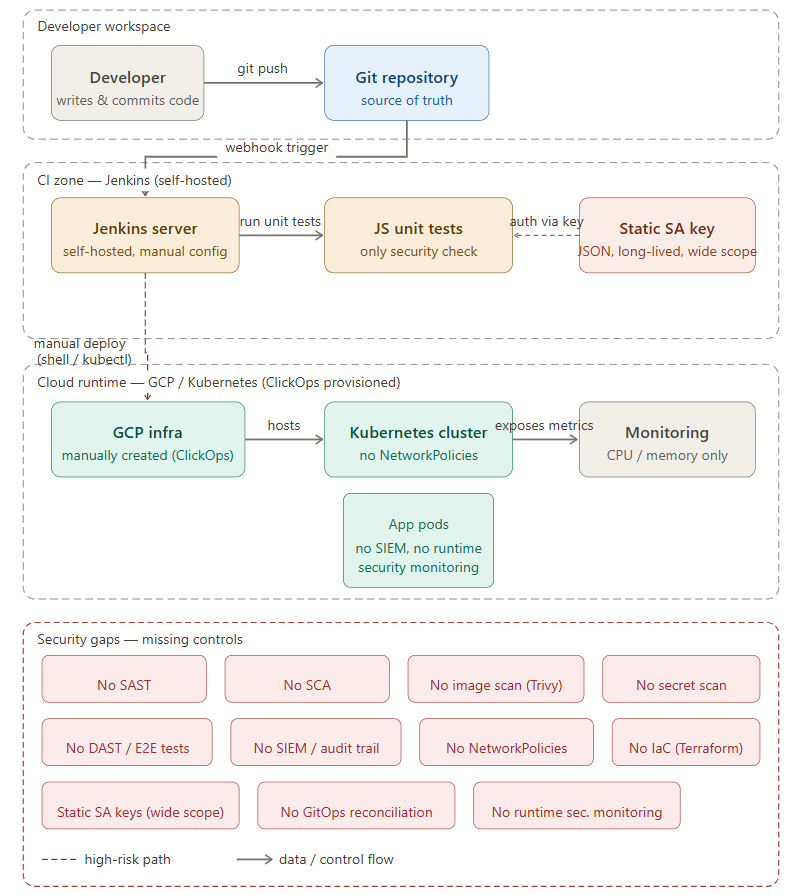
\includegraphics[width=0.9\textwidth,keepaspectratio]{images/old_jenkins_logical_architecture}
    \caption{Architecture logique de l'approche Jenkins (état initial)}
    \label{fig:jenkins_architecture_existant}
\end{figure}

Le tableau \ref{tab:etat_avant} synthétise l'état de l'art avant la transformation:

\begin{table}[h]
    \centering
    \setlength{\arrayrulewidth}{0.8pt}
    \setlength{\dashlinedash}{3pt}
    \setlength{\dashlinegap}{2pt}
    \renewcommand{\arraystretch}{1.4}
    \caption{État du système avant la transformation DevSecOps}
    \label{tab:etat_avant}
    \begin{tabularx}{\textwidth}{|>{\centering\arraybackslash}X|>{\centering\arraybackslash}X|}
\hline
\tableheader \textbf{Aspect} & \textbf{État Avant} \\
\hline
Outil CI & Jenkins (auto-hébergé, configuration manuelle) \\ \hdashline
Tests & Tests BDD uniquement (framework T4T interne) \\ \hdashline
Sécurité & \textbf{Aucune} \\ \hdashline
Scan de vulnérabilités & Absent \\ \hdashline
Scan des images Docker & Absent \\ \hdashline
Scan des secrets & Absent \\ \hdashline
Tests E2E & Absents ou manuels \\ \hdashline
Infrastructure & Créée manuellement via console GCP (ClickOps) \\ \hdashline
Déploiement & Scripts shell ad-hoc, pas versionnés \\ \hdashline
Authentification CI & Clés JSON longue durée dans les secrets Jenkins \\ \hdashline
Monitoring & Basique (CPU/mémoire uniquement) \\ \hdashline
Sécurité réseau & Pas de NetworkPolicies \\ \hdashline
SIEM & Absent \\ \hdashline
Audit trail & Inexistant \\
\hline
    \end{tabularx}
\end{table}

\subsection{Problèmes Identifiés}

\textbf{Problème 1 --- Absence totale de sécurité dans le pipeline:}
Le pipeline Jenkins se contentait de vérifier que les tests BDD T4T passaient. Aucune analyse
statique de sécurité (SAST), aucun scan de dépendances (SCA), aucun scan d'images Docker
n'était effectué. Des vulnérabilités critiques pouvaient transiter du code source jusqu'en
production sans être détectées.

\textbf{Problème 2 --- Clés d'authentification statiques:}
Jenkins utilisait des clés JSON Google Cloud Service Account avec des permissions larges, stockées
en clair dans la configuration Jenkins. La compromission de ces clés aurait donné un accès complet
à l'infrastructure GCP.

\textbf{Problème 3 --- Infrastructure non reproductible:}
Les ressources GCP (cluster Kubernetes, réseau, IAM) étaient créées manuellement via la console.
Il était impossible de recréer l'environnement de façon fiable, et les modifications n'étaient
pas tracées.

\textbf{Problème 4 --- Déploiements impératifs non versionnés:}
Les déploiements étaient effectués via des commandes \texttt{kubectl apply} ou des scripts shell
non versionnés, sans historique, sans rollback automatique et sans validation de l'état désiré.

\textbf{Problème 5 --- Aucune visibilité sur la sécurité en production:}
Après le déploiement, aucun outil ne surveillait les comportements anormaux, les tentatives
d'intrusion ou les événements de sécurité sur les nœuds Kubernetes.

\textbf{Problème 6 --- Tests non représentatifs:}
Les tests BDD T4T ne couvraient que les scénarios fonctionnels métier, sans jamais valider
le comportement réel de l'application dans son contexte de déploiement cloud-native.
Aucun test de sécurité, aucun test E2E dans le cluster, et aucun scan dynamique n'étaient
réalisés. De plus, aucun rapport d'analyse de sécurité n'était généré.

\subsection{Dette Technique et Sécuritaire Accumulée}

 Le tableau \ref{tab:owasp_avant} résume la dette accumulée selon les catégories OWASP Top 10:

\begin{table}[h]
    \centering
    \setlength{\arrayrulewidth}{0.8pt}
    \setlength{\dashlinedash}{3pt}
    \setlength{\dashlinegap}{2pt}
    \renewcommand{\arraystretch}{1.4}
    \caption{Couverture OWASP Top 10 avant ce projet}
    \label{tab:owasp_avant}
    \begin{tabularx}{\textwidth}{|>{\centering\arraybackslash}X|>{\centering\arraybackslash}X|}
\hline
\tableheader \textbf{Catégorie OWASP} & \textbf{État Avant} \\
\hline
A01 - Broken Access Control & Non contrôlé (credentials hardcodés) \\ \hdashline
A02 - Cryptographic Failures & Secrets en clair dans le code et CI \\ \hdashline
A03 - Injection (XSS) & Non détecté, pas de SAST \\ \hdashline
A05 - Security Misconfiguration & Containers root, pas de NetworkPolicies \\ \hdashline
A06 - Vulnerable Components & Dépendances jamais auditées \\ \hdashline
A08 - Software Integrity Failures & Images non signées, pas de SBOM \\ \hdashline
A09 - Security Logging Failures & Aucun SIEM, aucun audit trail \\
\hline
    \end{tabularx}
\end{table}


\section*{Conclusion}

Ce chapitre a établi le contexte général du projet en identifiant les six lacunes majeures de
l'approche Jenkins initiale et en formulant la problématique centrale~: intégrer la sécurité
à chaque étape du cycle de livraison sans sacrifier la vélocité.
L'analyse de la dette technique
et sécuritaire accumulée, notamment au regard du référentiel OWASP Top 10, justifie pleinement
l'ampleur de la transformation entreprise.
Le chapitre suivant présente l'analyse des besoins
fonctionnels et non fonctionnels identifiés pour répondre à cette problématique.


    \clearpage

    %% Chapitre 2
    \chapter{Analyse des Besoins}
    \label{chap:besoins}
    %% ============================================================
%%  CHAPITRE 2 — Analyse des Besoins (Requirement Analysis)
%% ============================================================

\section*{Introduction}

Ce chapitre présente l'analyse des besoins du projet. À partir de la problématique identifiée
au chapitre précédent, nous identifions les acteurs impliqués, formulons les besoins fonctionnels
et non fonctionnels, modélisons les cas d'utilisation, et décrivons la méthodologie Agile
adoptée pour organiser la réalisation du projet en sprints itératifs.


\section{Identification des Acteurs}

Trois catégories d'acteurs interagissent avec la plateforme DevSecOps~:

\begin{table}[h]
    \centering
    \setlength{\arrayrulewidth}{0.8pt}
    \setlength{\dashlinedash}{3pt}
    \setlength{\dashlinegap}{2pt}
    \renewcommand{\arraystretch}{1.4}
    \caption{Acteurs du système et leurs rôles}
    \label{tab:acteurs}
    \begin{tabularx}{\textwidth}{|>{\centering\arraybackslash}X|>{\centering\arraybackslash}X|>{\centering\arraybackslash}X|}
\hline
\tableheader \textbf{Acteur} & \textbf{Type} & \textbf{Rôle} \\
\hline
Développeur & Humain & Écrit le code, pousse les commits, consulte les rapports de sécurité \\ \hdashline
Ingénieur DevOps / DevSecOps & Humain & Configure l'infrastructure, le pipeline et les politiques de sécurité \\ \hdashline
Pipeline CI/CD (GitHub Actions) & Système & Exécute automatiquement les builds, scans et déploiements \\ \hdashline
Argo CD & Système & Réconcilie l'état du cluster avec l'état désiré dans Git \\ \hdashline
Utilisateur final & Humain & Utilise l'application Todo App via le navigateur \\
\hline
    \end{tabularx}
\end{table}


\section{Besoins Fonctionnels}

Les besoins fonctionnels couvrent les capacités que la plateforme doit offrir. Ils sont
organisés par domaine dans le tableau~\ref{tab:besoins_fonctionnels}~:

\begin{table}[H]
    \centering
    \setlength{\arrayrulewidth}{0.8pt}
    \setlength{\dashlinedash}{3pt}
    \setlength{\dashlinegap}{2pt}
    \renewcommand{\arraystretch}{1.4}
    \caption{Besoins fonctionnels du projet}
    \label{tab:besoins_fonctionnels}
    \begin{tabularx}{\textwidth}{|>{\centering\arraybackslash}X|>{\centering\arraybackslash}X|>{\centering\arraybackslash}X|}
\hline
\tableheader \textbf{ID} & \textbf{Besoin Fonctionnel} & \textbf{Domaine} \\
\hline
BF-01 & Provisionner l'infrastructure GCP de manière reproductible via du code & Infrastructure \\ \hdashline
BF-02 & Construire et publier automatiquement les images Docker à chaque push & CI/CD \\ \hdashline
BF-03 & Exécuter des tests unitaires automatiquement à chaque commit & CI/CD \\ \hdashline
BF-04 & Scanner le code source pour détecter les vulnérabilités (SAST) & Sécurité \\ \hdashline
BF-05 & Scanner les dépendances npm et les images Docker pour les CVEs (SCA) & Sécurité \\ \hdashline
BF-06 & Scanner l'application déployée en boîte noire (DAST) & Sécurité \\ \hdashline
BF-07 & Déployer automatiquement l'application via GitOps (Argo CD) & Déploiement \\ \hdashline
BF-08 & Exécuter des tests E2E dans le cluster après chaque déploiement & Tests \\ \hdashline
BF-09 & Collecter et visualiser les métriques de l'application en temps réel & Observabilité \\ \hdashline
BF-10 & Surveiller les événements de sécurité en production (SIEM) & Sécurité \\ \hdashline
BF-11 & Permettre l'authentification, la gestion de tâches (CRUD) et la persistance & Application \\
\hline
    \end{tabularx}
\end{table}


\section{Besoins Non Fonctionnels}

Les besoins non fonctionnels définissent les contraintes de qualité de la plateforme~:

\begin{table}[H]
    \centering
    \setlength{\arrayrulewidth}{0.8pt}
    \setlength{\dashlinedash}{3pt}
    \setlength{\dashlinegap}{2pt}
    \renewcommand{\arraystretch}{1.4}
    \caption{Besoins non fonctionnels du projet}
    \label{tab:besoins_non_fonctionnels}
    \begin{tabularx}{\textwidth}{|>{\centering\arraybackslash}X|>{\centering\arraybackslash}X|>{\centering\arraybackslash}X|}
\hline
\tableheader \textbf{ID} & \textbf{Besoin Non Fonctionnel} & \textbf{Catégorie} \\
\hline
BNF-01 & Zéro clé d'authentification statique dans le pipeline (Keyless) & Sécurité \\ \hdashline
BNF-02 & Réseau Zero Trust~: tout trafic interdit par défaut, flux explicites & Sécurité \\ \hdashline
BNF-03 & Auto-scaling horizontal de 2 à 8 replicas selon la charge CPU & Performance \\ \hdashline
BNF-04 & Infrastructure 100\% reproductible à partir du code source & Fiabilité \\ \hdashline
BNF-05 & Chaque build, scan et déploiement doit produire un rapport auditable & Auditabilité \\ \hdashline
BNF-06 & Détection automatique et correction du drift de configuration (self-heal) & Résilience \\ \hdashline
BNF-07 & Couverture de tests unitaires $\geq$ 70\% & Qualité \\ \hdashline
BNF-08 & Temps de détection d'une CVE critique < 5 minutes & Sécurité \\ \hdashline
BNF-09 & Rollback automatique via Git revert + Argo CD & Disponibilité \\
\hline
    \end{tabularx}
\end{table}


\section{Diagramme de Cas d'Utilisation Global}

Le diagramme de cas d'utilisation global modélise les interactions entre les acteurs
et les principales fonctionnalités de la plateforme DevSecOps.

\begin{figure}[H]
    \centering
    \fbox{\parbox{0.85\textwidth}{\centering
        \vspace{3cm}
        Espace réservé pour la Figure~\ref{fig:use_case_global}\\
        \textbf{Diagramme de cas d'utilisation global}\\[6pt]
        \footnotesize Acteurs~: Développeur, Ingénieur DevSecOps, Utilisateur final,\\
        Pipeline CI/CD (système), Argo CD (système)\\[6pt]
        Cas d'utilisation~: Pousser du code, Construire \& tester, Scanner la sécurité,\\
        Déployer via GitOps, Surveiller, Gérer les tâches Todo
        \vspace{3cm}
    }}
    \caption{Diagramme de cas d'utilisation global de la plateforme DevSecOps}
    \label{fig:use_case_global}
\end{figure}


\section{Cas d'Utilisation Détaillés}

\subsection{CU-01~: Pousser du Code et Déclencher le Pipeline}

\begin{table}[H]
    \centering
    \setlength{\arrayrulewidth}{0.8pt}
    \renewcommand{\arraystretch}{1.4}
    \caption{Description du cas d'utilisation CU-01}
    \label{tab:cu01}
    \begin{tabularx}{\textwidth}{|>{\raggedright\arraybackslash}p{3.5cm}|X|}
\hline
\tableheader \textbf{Champ} & \textbf{Description} \\
\hline
Titre & Pousser du code et déclencher le pipeline \\
\hline
Acteur principal & Développeur \\
\hline
Précondition & Le développeur a un accès au dépôt Git \\
\hline
Scénario nominal & 1. Le développeur pousse un commit sur la branche principale \newline
2. GitHub Actions détecte le push et démarre le pipeline \newline
3. Le job \texttt{build-test} exécute lint, tests unitaires, SonarCloud et Trivy FS \newline
4. En cas de succès, le job \texttt{app-image-release} construit et publie l'image Docker \newline
5. Le job \texttt{update-k8s-tags} met à jour les manifests Kubernetes \\
\hline
Postcondition & L'image Docker est publiée, les manifests K8s sont mis à jour dans Git \\
\hline
Scénario alternatif & Si un test échoue ou un scan critique bloque, le pipeline s'arrête et notifie le développeur \\
\hline
    \end{tabularx}
\end{table}

\subsection{CU-02~: Déployer via GitOps}

\begin{table}[H]
    \centering
    \setlength{\arrayrulewidth}{0.8pt}
    \renewcommand{\arraystretch}{1.4}
    \caption{Description du cas d'utilisation CU-02}
    \label{tab:cu02}
    \begin{tabularx}{\textwidth}{|>{\raggedright\arraybackslash}p{3.5cm}|X|}
\hline
\tableheader \textbf{Champ} & \textbf{Description} \\
\hline
Titre & Déployer automatiquement via GitOps \\
\hline
Acteur principal & Argo CD (système) \\
\hline
Précondition & Les manifests K8s dans Git ont été mis à jour avec le nouveau tag d'image \\
\hline
Scénario nominal & 1. Argo CD détecte un changement dans le dépôt Git \newline
2. Argo CD compare l'état désiré (Git) avec l'état réel du cluster \newline
3. Argo CD synchronise automatiquement les ressources Kubernetes \newline
4. Les hooks PostSync lancent les tests Playwright E2E \newline
5. Le dashboard Argo CD affiche l'état synchronisé \\
\hline
Postcondition & L'application est déployée, les tests E2E sont validés \\
\hline
Scénario alternatif & En cas de drift détecté, Argo CD applique le self-heal automatiquement \\
\hline
    \end{tabularx}
\end{table}

\subsection{CU-03~: Gérer les Tâches Todo}

\begin{table}[H]
    \centering
    \setlength{\arrayrulewidth}{0.8pt}
    \renewcommand{\arraystretch}{1.4}
    \caption{Description du cas d'utilisation CU-03}
    \label{tab:cu03}
    \begin{tabularx}{\textwidth}{|>{\raggedright\arraybackslash}p{3.5cm}|X|}
\hline
\tableheader \textbf{Champ} & \textbf{Description} \\
\hline
Titre & Gérer les tâches Todo (CRUD) \\
\hline
Acteur principal & Utilisateur final \\
\hline
Précondition & L'utilisateur est authentifié sur l'application \\
\hline
Scénario nominal & 1. L'utilisateur ajoute une nouvelle tâche \newline
2. L'utilisateur coche une tâche comme complétée \newline
3. L'utilisateur supprime une tâche \newline
4. Les données persistent via localStorage après rechargement \\
\hline
Postcondition & Les tâches sont sauvegardées et visibles \\
\hline
Scénario alternatif & Si l'utilisateur n'est pas authentifié, il est redirigé vers la page de login \\
\hline
    \end{tabularx}
\end{table}


\section{Méthodologie de Travail~: Scrum Agile}

\subsection{Choix de la Méthodologie}

Le projet suit la méthodologie \textbf{Scrum} pour sa capacité à gérer la complexité
de manière itérative et incrémentale. Chaque sprint livre un incrément fonctionnel et
testable, permettant de valider progressivement les composantes de la plateforme DevSecOps.

\begin{figure}[H]
    \centering
    \fbox{\parbox{0.85\textwidth}{\centering
        \vspace{2.5cm}
        Espace réservé pour la Figure~\ref{fig:scrum_process}\\
        \textbf{Processus Scrum appliqué au projet}\\[6pt]
        \footnotesize Product Backlog $\to$ Sprint Planning $\to$ Sprint (2--3 semaines)\\
        $\to$ Sprint Review $\to$ Sprint Retrospective $\to$ Incrément livré
        \vspace{2.5cm}
    }}
    \caption{Processus Scrum appliqué au projet}
    \label{fig:scrum_process}
\end{figure}

\subsection{Équipe Scrum}

\begin{table}[H]
    \centering
    \setlength{\arrayrulewidth}{0.8pt}
    \setlength{\dashlinedash}{3pt}
    \setlength{\dashlinegap}{2pt}
    \renewcommand{\arraystretch}{1.4}
    \caption{Composition de l'équipe Scrum}
    \label{tab:equipe_scrum}
    \begin{tabularx}{\textwidth}{|>{\centering\arraybackslash}X|>{\centering\arraybackslash}X|>{\centering\arraybackslash}X|}
\hline
\tableheader \textbf{Rôle Scrum} & \textbf{Personne} & \textbf{Responsabilité} \\
\hline
Product Owner & Encadrant professionnel (Sopra Steria) & Définition des priorités et validation des livrables \\ \hdashline
Scrum Master & Encadrant académique (ESPRIT) & Suivi méthodologique et levée des blocages \\ \hdashline
Développeur & NAFFATI & Conception, implémentation et tests \\
\hline
    \end{tabularx}
\end{table}

\subsection{Planification des Sprints}

Le projet est découpé en \textbf{quatre sprints} de 2 à 3 semaines chacun, couvrant
l'ensemble des besoins identifiés~:

\begin{table}[H]
    \centering
    \setlength{\arrayrulewidth}{0.8pt}
    \setlength{\dashlinedash}{3pt}
    \setlength{\dashlinegap}{2pt}
    \renewcommand{\arraystretch}{1.4}
    \caption{Planification des sprints du projet}
    \label{tab:sprints}
    \begin{tabularx}{\textwidth}{|>{\centering\arraybackslash}X|>{\centering\arraybackslash}X|>{\centering\arraybackslash}X|>{\centering\arraybackslash}X|}
\hline
\tableheader \textbf{Sprint} & \textbf{Durée} & \textbf{Objectif} & \textbf{Besoins couverts} \\
\hline
Sprint 1 & 3 semaines & Infrastructure as Code et cluster GKE & BF-01, BNF-04 \\ \hdashline
Sprint 2 & 3 semaines & Containerisation, pipeline CI/CD et authentification Keyless & BF-02, BF-03, BNF-01, BNF-05 \\ \hdashline
Sprint 3 & 3 semaines & Sécurité intégrée (SAST, SCA, DAST), GitOps et réseau Zero Trust & BF-04, BF-05, BF-06, BF-07, BNF-02, BNF-06 \\ \hdashline
Sprint 4 & 2 semaines & Tests E2E, observabilité, SIEM et bilan & BF-08, BF-09, BF-10, BNF-03, BNF-07, BNF-08, BNF-09 \\
\hline
    \end{tabularx}
\end{table}

\subsection{Product Backlog}

Le Product Backlog regroupe l'ensemble des \textit{User Stories} priorisées par le
Product Owner. Le tableau~\ref{tab:backlog} présente les éléments principaux~:

\begin{table}[H]
    \centering
    \setlength{\arrayrulewidth}{0.8pt}
    \setlength{\dashlinedash}{3pt}
    \setlength{\dashlinegap}{2pt}
    \renewcommand{\arraystretch}{1.4}
    \caption{Product Backlog (extrait)}
    \label{tab:backlog}
    \begin{tabularx}{\textwidth}{|>{\centering\arraybackslash}X|>{\centering\arraybackslash}X|>{\centering\arraybackslash}X|>{\centering\arraybackslash}X|}
\hline
\tableheader \textbf{ID} & \textbf{User Story} & \textbf{Priorité} & \textbf{Sprint} \\
\hline
US-01 & En tant que DevOps, je veux provisionner l'infra via Terraform & Haute & 1 \\ \hdashline
US-02 & En tant que DevOps, je veux un cluster GKE Autopilot opérationnel & Haute & 1 \\ \hdashline
US-03 & En tant que Dev, je veux un Dockerfile multi-stage optimisé & Haute & 2 \\ \hdashline
US-04 & En tant que Dev, je veux un pipeline CI qui build et teste à chaque push & Haute & 2 \\ \hdashline
US-05 & En tant que DevSecOps, je veux une auth CI sans clé statique (WIF) & Haute & 2 \\ \hdashline
US-06 & En tant que DevSecOps, je veux des scans SAST/SCA automatiques & Haute & 3 \\ \hdashline
US-07 & En tant que DevSecOps, je veux un déploiement GitOps avec Argo CD & Haute & 3 \\ \hdashline
US-08 & En tant que DevSecOps, je veux un réseau Zero Trust (NetworkPolicies) & Moyenne & 3 \\ \hdashline
US-09 & En tant que DevSecOps, je veux un scan DAST post-déploiement (ZAP) & Moyenne & 3 \\ \hdashline
US-10 & En tant que QA, je veux 6 scénarios Playwright E2E in-cluster & Moyenne & 4 \\ \hdashline
US-11 & En tant que Ops, je veux Prometheus + Grafana pour l'observabilité & Moyenne & 4 \\ \hdashline
US-12 & En tant que SecOps, je veux Wazuh SIEM pour la surveillance runtime & Moyenne & 4 \\
\hline
    \end{tabularx}
\end{table}

\begin{figure}[H]
    \centering
    \fbox{\parbox{0.85\textwidth}{\centering
        \vspace{2.5cm}
        Espace réservé pour la Figure~\ref{fig:gantt}\\
        \textbf{Diagramme de Gantt du projet}\\[6pt]
        \footnotesize Sprint 1 (semaines 1--3) | Sprint 2 (semaines 4--6) |\\
        Sprint 3 (semaines 7--9) | Sprint 4 (semaines 10--11)
        \vspace{2.5cm}
    }}
    \caption{Diagramme de Gantt de la planification des sprints}
    \label{fig:gantt}
\end{figure}


\section*{Conclusion}

Ce chapitre a formalisé les besoins du projet à travers onze besoins fonctionnels et neuf
besoins non fonctionnels, identifié les acteurs du système, et modélisé les cas d'utilisation
clés. La méthodologie Scrum adoptée organise la réalisation en quatre sprints itératifs,
chacun livrant un incrément fonctionnel et testable. Le chapitre suivant présente l'analyse
et la conception détaillée du système.

    \clearpage

    %% Chapitre 3
    \chapter{Analyse et Conception du Système}
    \label{chap:conception}
    %% ============================================================
%%  CHAPITRE 3 — Analyse et Conception du Système
%% ============================================================

\section*{Introduction}

Ce chapitre présente l'analyse et la conception détaillée du système. Nous y définissons
les fondements du DevSecOps et le principe Shift-Left, décrivons l'architecture globale en
six couches, l'architecture physique sur Google Cloud Platform, l'architecture logique
Kubernetes, les diagrammes UML de conception (séquence, activité, déploiement), le stack
technique de l'application cible, et les choix technologiques justifiés.


\section{Définition du DevSecOps et Principe Shift-Left}

\textbf{DevSecOps} est une extension de la philosophie DevOps qui intègre la sécurité
(\textbf{Sec}) comme responsabilité partagée, continue et automatisée dans le cycle de
développement. L'idée fondamentale est le \textbf{Shift-Left}~: déplacer les contrôles
de sécurité le plus tôt possible dans le cycle, là où les corrections sont les moins coûteuses.

\begin{figure}[H]
    \centering
    \fbox{\parbox{0.85\textwidth}{\centering
        \vspace{2.5cm}
        Espace réservé pour la Figure~\ref{fig:shiftleft}\\
        \textbf{Principe Shift-Left de la sécurité dans le cycle DevSecOps}\\[6pt]
        \footnotesize Plan $\to$ Code $\to$ Build $\to$ Test $\to$ Release $\to$ Deploy $\to$ Monitor\\
        Sec Review | SAST/Lint | SCA/Trivy | DAST/ZAP | cosign | K8s Sec | SIEM/Wazuh
        \vspace{2.5cm}
    }}
    \caption{Principe Shift-Left de la sécurité dans le cycle DevSecOps}
    \label{fig:shiftleft}
\end{figure}


\section{Les Huit Principes Directeurs du Projet}

Le tableau~\ref{tab:principes} présente les huit principes directeurs qui guident la conception
de la solution~:

\begin{table}[H]
\centering
\setlength{\arrayrulewidth}{0.8pt}
\setlength{\dashlinedash}{3pt}
\setlength{\dashlinegap}{2pt}
\renewcommand{\arraystretch}{1.4}
\caption{Huit principes directeurs de la plateforme DevSecOps}
\label{tab:principes}
\begin{tabularx}{\textwidth}{|>{\centering\arraybackslash}X|>{\centering\arraybackslash}X|>{\centering\arraybackslash}X|}
\hline
\tableheader \textbf{\#} & \textbf{Principe} & \textbf{Implémentation} \\
\hline
1 & Tout est Code & Terraform pour l'infra, YAML pour K8s, tout versionné dans Git \\ \hdashline
2 & Sécurité Shift-Left & Trivy + SonarCloud dès le build, avant tout déploiement \\ \hdashline
3 & Keyless First & Workload Identity Federation --- zéro clé JSON statique \\ \hdashline
4 & Zero Trust Réseau & NetworkPolicies default-deny, flux explicitement autorisés \\ \hdashline
5 & GitOps & Argo CD comme seul moteur de réconciliation du cluster \\ \hdashline
6 & Tests au plus proche du réel & Playwright E2E dans le cluster, PostSync hooks \\ \hdashline
7 & Observabilité Continue & Prometheus + Grafana + Wazuh en permanence \\ \hdashline
8 & Preuves Auditables & Chaque outil génère des rapports uploadés comme artefacts CI \\
\hline
\end{tabularx}
\end{table}


\section{Architecture Globale en Six Couches}

La solution s'articule autour de \textbf{six couches complémentaires} illustrées dans
la figure~\ref{fig:couches}~:

\begin{figure}[H]
    \centering
    \fbox{\parbox{0.85\textwidth}{\centering
        \vspace{3cm}
        Espace réservé pour la Figure~\ref{fig:couches}\\
        \textbf{Architecture en six couches de la plateforme DevSecOps}\\[6pt]
        \footnotesize
        Couche 6~: Sécurité Runtime (Wazuh, NetworkPolicies, Workload Identity)\\
        Couche 5~: Observabilité (Prometheus, Grafana, nginx-exporter)\\
        Couche 4~: Orchestration (GKE Autopilot, Namespaces, HPA, Ingress)\\
        Couche 3~: Livraison (GitHub Actions, Argo CD, Artifact Registry)\\
        Couche 2~: Sécurité Applicative (Trivy, OWASP ZAP, SonarCloud, Playwright)\\
        Couche 1~: Infrastructure (Terraform, GCP VPC, GKE, IAM, Artifact Registry)
        \vspace{3cm}
    }}
    \caption{Architecture en six couches de la plateforme DevSecOps}
    \label{fig:couches}
\end{figure}


\section{Architecture Physique GCP}

L'infrastructure est déployée sur le projet GCP \texttt{pfe-esprit-489411} dans la région
\texttt{europe-west1}. Elle comprend les composants suivants~:

\begin{itemize}
  \item \textbf{VPC \texttt{devops-vpc}}~: réseau dédié avec subnet \texttt{devops-subnet}~;
        plages secondaires pour les nœuds (\texttt{10.10.0.0/20}), pods (\texttt{10.20.0.0/16})
        et services (\texttt{10.30.0.0/20})~;
  \item \textbf{Cluster GKE Autopilot \texttt{devops-cluster}}~: mode géré, patches de
        sécurité automatiques, facturation à la ressource pod~;
  \item \textbf{Artifact Registry}~: stockage des images Docker de l'application et des tests~;
  \item \textbf{VM Compute Engine}~: hébergement du manager Wazuh SIEM
        (\texttt{e2-medium}, IP \texttt{10.10.0.2}).
\end{itemize}

\begin{figure}[H]
    \centering
    \fbox{\parbox{0.85\textwidth}{\centering
        \vspace{3cm}
        Espace réservé pour la Figure~\ref{fig:archi_physique}\\
        \textbf{Architecture physique GCP}\\[6pt]
        \footnotesize GCP Project $\to$ VPC devops-vpc $\to$ Subnet devops-subnet\\
        GKE Autopilot Cluster | Artifact Registry | Wazuh VM (e2-medium)\\
        Workload Identity Federation $\leftrightarrow$ GitHub Actions
        \vspace{3cm}
    }}
    \caption{Architecture physique de l'infrastructure GCP}
    \label{fig:archi_physique}
\end{figure}


\section{Architecture Logique Kubernetes}

Le cluster est segmenté en \textbf{cinq namespaces fonctionnels} avec des responsabilités
strictement séparées, comme présenté dans le tableau~\ref{tab:namespaces}~:

\begin{table}[H]
\centering
\setlength{\arrayrulewidth}{0.8pt}
\setlength{\dashlinedash}{3pt}
\setlength{\dashlinegap}{2pt}
\renewcommand{\arraystretch}{1.4}
\caption{Organisation en namespaces Kubernetes}
\label{tab:namespaces}
\begin{tabularx}{\textwidth}{|>{\centering\arraybackslash}X|>{\centering\arraybackslash}X|>{\centering\arraybackslash}X|}
\hline
\tableheader \textbf{Namespace} & \textbf{Rôle} & \textbf{Ressources principales} \\
\hline
\texttt{app} & Workload applicatif & Deployment, Service, Ingress, HPA, PostSync Job \\ \hdashline
\texttt{testing} & Validation E2E & Playwright Job, ServiceAccount \\ \hdashline
\texttt{observability} & Collecte de métriques & Prometheus, Grafana, ServiceMonitor \\ \hdashline
\texttt{security} & Politiques et SIEM & NetworkPolicies, Wazuh Agent DaemonSet \\ \hdashline
\texttt{argocd} & Moteur GitOps & Argo CD Applications \\
\hline
\end{tabularx}
\end{table}

\begin{figure}[H]
    \centering
    \fbox{\parbox{0.85\textwidth}{\centering
        \vspace{3cm}
        Espace réservé pour la Figure~\ref{fig:archi_k8s}\\
        \textbf{Diagramme d'architecture logique Kubernetes}\\[6pt]
        \footnotesize 5 namespaces~: app, testing, observability, security, argocd\\
        Flux réseau~: testing $\to$ app (TCP 80), observability $\to$ app (TCP 9113),\\
        security $\to$ Wazuh VM (TCP 1514), Ingress $\to$ app (TCP 80)
        \vspace{3cm}
    }}
    \caption{Architecture logique du cluster Kubernetes}
    \label{fig:archi_k8s}
\end{figure}


\section{Diagrammes de Conception}

\subsection{Diagramme de Séquence~: Pipeline CI/CD Complet}

Le diagramme de séquence suivant modélise le flux complet du pipeline CI/CD, depuis le
push du développeur jusqu'au déploiement GitOps et les tests E2E.

\begin{figure}[H]
    \centering
    \fbox{\parbox{0.85\textwidth}{\centering
        \vspace{4cm}
        Espace réservé pour la Figure~\ref{fig:seq_pipeline}\\
        \textbf{Diagramme de séquence~: Pipeline CI/CD complet}\\[6pt]
        \footnotesize Développeur $\to$ GitHub~: push commit\\
        GitHub $\to$ Actions~: déclencher pipeline\\
        Actions $\to$ SonarCloud~: scan SAST\\
        Actions $\to$ Trivy~: scan FS (SCA)\\
        Actions $\to$ Artifact Registry~: push image Docker\\
        Actions $\to$ Trivy~: scan image\\
        Actions $\to$ Git~: update K8s tags\\
        Argo CD $\to$ Git~: detect change\\
        Argo CD $\to$ GKE~: sync ressources\\
        Argo CD $\to$ Playwright~: PostSync E2E tests\\
        Actions $\to$ ZAP~: scan DAST
        \vspace{4cm}
    }}
    \caption{Diagramme de séquence du pipeline CI/CD complet}
    \label{fig:seq_pipeline}
\end{figure}

\subsection{Diagramme de Séquence~: Authentification Workload Identity Federation}

\begin{figure}[H]
    \centering
    \fbox{\parbox{0.85\textwidth}{\centering
        \vspace{3cm}
        Espace réservé pour la Figure~\ref{fig:seq_wif}\\
        \textbf{Diagramme de séquence~: Authentification WIF}\\[6pt]
        \footnotesize GitHub Actions $\to$ GitHub OIDC~: request JWT token\\
        GitHub Actions $\to$ GCP WIF Pool~: present JWT\\
        GCP WIF $\to$ GCP IAM~: verify issuer, repo, branch\\
        GCP IAM $\to$ GitHub Actions~: temporary credentials (1h)\\
        GitHub Actions $\to$ GCP APIs~: authenticated calls
        \vspace{3cm}
    }}
    \caption{Diagramme de séquence de l'authentification Workload Identity Federation}
    \label{fig:seq_wif}
\end{figure}

\subsection{Diagramme d'Activité~: Flux GitOps avec Argo CD}

\begin{figure}[H]
    \centering
    \fbox{\parbox{0.85\textwidth}{\centering
        \vspace{3cm}
        Espace réservé pour la Figure~\ref{fig:act_gitops}\\
        \textbf{Diagramme d'activité~: Flux GitOps Argo CD}\\[6pt]
        \footnotesize [Commit dans Git] $\to$ Argo CD détecte le changement $\to$\\
        Comparer état désiré vs état réel $\to$ [Si différence] Synchroniser $\to$\\
        Appliquer les manifests K8s $\to$ Exécuter PostSync hooks (Playwright) $\to$\\
        [Si drift détecté] Self-heal automatique $\to$ État synchronisé
        \vspace{3cm}
    }}
    \caption{Diagramme d'activité du flux GitOps avec Argo CD}
    \label{fig:act_gitops}
\end{figure}

\subsection{Diagramme de Déploiement}

\begin{figure}[H]
    \centering
    \fbox{\parbox{0.85\textwidth}{\centering
        \vspace{3.5cm}
        Espace réservé pour la Figure~\ref{fig:deployment_diagram}\\
        \textbf{Diagramme de déploiement UML}\\[6pt]
        \footnotesize
        \textbf{Nœud GitHub}~: Actions Runner, OIDC Provider\\
        \textbf{Nœud GCP}~: VPC devops-vpc\\
        \quad \textbf{GKE Cluster}~: ns app (Deployment + nginx-exporter sidecar),\\
        \quad\quad ns testing (Playwright Job), ns observability (Prometheus, Grafana),\\
        \quad\quad ns security (Wazuh Agent), ns argocd (Argo CD)\\
        \quad \textbf{VM Wazuh}~: Wazuh Manager (TCP 1514)\\
        \quad \textbf{Artifact Registry}~: Docker images\\
        \textbf{Nœud Externe}~: Navigateur utilisateur $\to$ Ingress GCE
        \vspace{3.5cm}
    }}
    \caption{Diagramme de déploiement de la plateforme}
    \label{fig:deployment_diagram}
\end{figure}


\section{L'Application Cible~: Todo App React}

\subsection{Description Fonctionnelle}

L'application déployée est une \textbf{Todo App} avec un portail de connexion, développée
avec React 18 et TypeScript. Cette application a été conçue comme \textbf{support de
démonstration} pour valider l'ensemble de la chaîne DevSecOps. En effet, l'équipe QA
utilise au quotidien le framework BDD interne \textbf{T4T} pour tester les applications RH
de production~; la Todo App permet de concevoir et de valider les pipelines DevSecOps dans un
environnement maîtrisé, avant de transposer ces pratiques aux projets réels de l'équipe.

Bien que fonctionnellement simple, l'application sert de support idéal car elle possède~:

\begin{itemize}
  \item Une \textbf{authentification} (cible pour les tests de sécurité)~;
  \item Une \textbf{interaction utilisateur} (cible pour les tests E2E et XSS)~;
  \item Une \textbf{persistance de données} via localStorage (cible pour les vulnérabilités
        de stockage)~;
  \item Une \textbf{chaîne de dépendances npm} (cible pour le SCA).
\end{itemize}

\begin{figure}[H]
    \centering
    \fbox{\parbox{0.85\textwidth}{\centering
        \vspace{2.5cm}
        Espace réservé pour la Figure~\ref{fig:app_screenshot_login}\\
        \textbf{Capture d'écran~: Page de login de la Todo App}
        \vspace{2.5cm}
    }}
    \caption{Page de login de la Todo App}
    \label{fig:app_screenshot_login}
\end{figure}

\begin{figure}[H]
    \centering
    \fbox{\parbox{0.85\textwidth}{\centering
        \vspace{2.5cm}
        Espace réservé pour la Figure~\ref{fig:app_screenshot_dashboard}\\
        \textbf{Capture d'écran~: Dashboard Todo avec liste de tâches}
        \vspace{2.5cm}
    }}
    \caption{Dashboard de gestion des tâches Todo}
    \label{fig:app_screenshot_dashboard}
\end{figure}

\subsection{Diagramme de Classes de l'Application}

\begin{figure}[H]
    \centering
    \fbox{\parbox{0.85\textwidth}{\centering
        \vspace{3cm}
        Espace réservé pour la Figure~\ref{fig:class_diagram}\\
        \textbf{Diagramme de classes de la Todo App}\\[6pt]
        \footnotesize Classes~: App, AuthContext, AuthProvider, LoginPage,\\
        TodoDashboard, TodoItem, Todo (interface)\\
        Relations~: App $\to$ AuthProvider $\to$ LoginPage / TodoDashboard\\
        TodoDashboard $\to$ TodoItem[] , TodoItem $\to$ Todo
        \vspace{3cm}
    }}
    \caption{Diagramme de classes de l'application Todo App}
    \label{fig:class_diagram}
\end{figure}

\subsection{Stack Technique}

Le tableau~\ref{tab:stack} détaille les technologies utilisées~:

\begin{table}[H]
\centering
\setlength{\arrayrulewidth}{0.8pt}
\setlength{\dashlinedash}{3pt}
\setlength{\dashlinegap}{2pt}
\renewcommand{\arraystretch}{1.4}
\caption{Stack technique de l'application}
\label{tab:stack}
\begin{tabularx}{\textwidth}{|>{\centering\arraybackslash}X|>{\centering\arraybackslash}X|>{\centering\arraybackslash}X|}
\hline
\tableheader \textbf{Couche} & \textbf{Technologie} & \textbf{Version} \\
\hline
Framework UI & React & 18.3.1 \\ \hdashline
Langage & TypeScript & 5.8.3 \\ \hdashline
Build tool & Vite & 8.0.0 \\ \hdashline
Styling & Tailwind CSS + Rosé Pine theme & 3.4.17 \\ \hdashline
Composants UI & shadcn/ui (Radix UI) & --- \\ \hdashline
Animations & Framer Motion & 12.x \\ \hdashline
Routing & React Router DOM & 6.30.1 \\ \hdashline
Gestionnaire de paquets & Bun & Latest \\ \hdashline
Serveur de production & Nginx & 1.21 (vulnérable intentionnel) \\
\hline
\end{tabularx}
\end{table}

\subsection{Vulnérabilités Intentionnelles}

\begin{warningbox}
Le composant \texttt{TodoItem} utilise intentionnellement \texttt{dangerouslySetInnerHTML}
pour rendre le texte des tâches, créant une vulnérabilité \textbf{XSS stockée} détectable
par OWASP ZAP et SonarCloud. De même, l'authentification est hardcodée côté client dans
\texttt{AuthContext.tsx}. Ces choix sont délibérés pour la démonstration des outils DevSecOps.
\end{warningbox}


\section{Choix Technologiques et Justifications}

\begin{table}[H]
\centering
\setlength{\arrayrulewidth}{0.8pt}
\setlength{\dashlinedash}{3pt}
\setlength{\dashlinegap}{2pt}
\renewcommand{\arraystretch}{1.4}
\caption{Choix technologiques et justifications}
\label{tab:choix_techno}
\begin{tabularx}{\textwidth}{|>{\centering\arraybackslash}X|>{\centering\arraybackslash}X|>{\centering\arraybackslash}X|}
\hline
\tableheader \textbf{Domaine} & \textbf{Outil choisi} & \textbf{Justification} \\
\hline
IaC & Terraform & Standard industriel, multi-cloud, état déclaratif \\ \hdashline
Orchestration & GKE Autopilot & Gestion nœuds par Google, sécurité par défaut, scaling auto \\ \hdashline
CI/CD & GitHub Actions & Natif GitHub, OIDC intégré, marketplace riche \\ \hdashline
GitOps & Argo CD & Self-heal, drift detection, UI dashboard, CNCF graduated \\ \hdashline
SAST & SonarCloud & Analyse TypeScript/React, Quality Gates, gratuit open-source \\ \hdashline
SCA + Container & Trivy & 3 modes (fs, image, config), SARIF output, open-source \\ \hdashline
DAST & OWASP ZAP & Standard industriel, baseline scan intégrable en CI \\ \hdashline
SIEM & Wazuh & Open-source, HIDS + FIM + compliance, compatible K8s \\ \hdashline
Observabilité & Prometheus + Grafana & Standard CNCF, écosystème exporters, dashboards \\ \hdashline
Tests E2E & Playwright & Multi-navigateur, conteneurisable, tags pour parallélisme \\
\hline
\end{tabularx}
\end{table}


\section{Comparaison Globale Avant/Après}

Le tableau~\ref{tab:avant_apres} offre une vue synthétique de la transformation conçue~:

\begin{table}[H]
\centering
\setlength{\arrayrulewidth}{0.8pt}
\setlength{\dashlinedash}{3pt}
\setlength{\dashlinegap}{2pt}
\renewcommand{\arraystretch}{1.4}
\caption{Comparaison des approches avant et après transformation}
\label{tab:avant_apres}
\begin{tabularx}{\textwidth}{|>{\centering\arraybackslash}X|>{\centering\arraybackslash}X|>{\centering\arraybackslash}X|}
\hline
\tableheader \textbf{Dimension} & \textbf{Avant (Jenkins)} & \textbf{Après (DevSecOps)} \\
\hline
Sécurité & Post-déploiement ou absente & Intégrée à chaque étape \\ \hdashline
Infrastructure & ClickOps manuel & Terraform IaC versionné \\ \hdashline
Déploiement & Scripts impératifs & GitOps déclaratif (Argo CD) \\ \hdashline
Tests & Unitaires seulement & Unit + E2E in-cluster + scans sécurité \\ \hdashline
Authentification & Clés JSON statiques & OIDC Workload Identity Federation \\ \hdashline
Réseau & Ouvert par défaut & Zero Trust (default-deny) \\ \hdashline
Monitoring & CPU/RAM basique & Métriques + SIEM + alertes \\ \hdashline
Audit trail & Inexistant & Chaque commit, build, déploiement tracé \\ \hdashline
Rollback & Manuel & Automatique via Git revert + Argo CD \\
\hline
\end{tabularx}
\end{table}


\section*{Conclusion}

Ce chapitre a présenté la conception détaillée du système~: une architecture DevSecOps en
six couches articulée autour de huit principes directeurs, une infrastructure GCP bien définie,
un cluster Kubernetes segmenté en cinq namespaces, et des diagrammes UML modélisant les flux
de livraison, de sécurité et de déploiement. Le chapitre suivant se consacre à l'implémentation
concrète de cette conception, organisée en quatre sprints Agile.

    \clearpage

    %% Chapitre 4
    \chapter{Implémentation et Réalisation par Sprints Agile}
    \label{chap:implementation}
    %% ============================================================
%%  CHAPITRE 4 — Implémentation et Réalisation par Sprints Agile
%% ============================================================

\section*{Introduction}

Ce chapitre décrit la réalisation concrète du projet, organisée en quatre sprints Agile.
Chaque sprint est présenté avec son backlog, les tâches réalisées, les extraits de code
ou de configuration pertinents, les captures d'écran des résultats, et une rétrospective.
Le chapitre se conclut par le bilan quantitatif global et les perspectives d'amélioration.


%% ================================================================
%%  SPRINT 1 — Infrastructure as Code et Cluster GKE
%% ================================================================
\section{Sprint 1~: Infrastructure as Code et Cluster GKE}

\subsection{Objectif et Backlog du Sprint}

\begin{table}[H]
\centering
\setlength{\arrayrulewidth}{0.8pt}
\setlength{\dashlinedash}{3pt}
\setlength{\dashlinegap}{2pt}
\renewcommand{\arraystretch}{1.4}
\caption{Backlog du Sprint 1}
\label{tab:backlog_s1}
\begin{tabularx}{\textwidth}{|>{\centering\arraybackslash}X|>{\centering\arraybackslash}X|>{\centering\arraybackslash}X|}
\hline
\tableheader \textbf{User Story} & \textbf{Tâche} & \textbf{Statut} \\
\hline
US-01~: Provisionner l'infra via Terraform & Écrire les modules Terraform (main, network, gke, iam, wif, wazuh) & Terminé \\ \hdashline
US-01 & Configurer le backend GCS pour le state distant & Terminé \\ \hdashline
US-02~: Cluster GKE Autopilot & Provisionner le cluster avec Workload Identity activé & Terminé \\ \hdashline
US-02 & Provisionner la VM Wazuh Manager & Terminé \\ \hdashline
US-02 & Créer les namespaces Kubernetes & Terminé \\
\hline
\end{tabularx}
\end{table}

\subsection{Infrastructure as Code avec Terraform}

\subsubsection{Justification du Choix Terraform}

Face à l'ancienne approche ClickOps, \textbf{Terraform} a été choisi pour provisionner
l'ensemble des ressources GCP de façon reproductible, versionnée et auditable.
Le tableau~\ref{tab:terraform_vs_clickops} compare les deux approches~:

\begin{table}[H]
\centering
\setlength{\arrayrulewidth}{0.8pt}
\setlength{\dashlinedash}{3pt}
\setlength{\dashlinegap}{2pt}
\renewcommand{\arraystretch}{1.4}
\caption{Comparaison ClickOps vs Terraform IaC}
\label{tab:terraform_vs_clickops}
\begin{tabularx}{\textwidth}{|>{\centering\arraybackslash}X|>{\centering\arraybackslash}X|>{\centering\arraybackslash}X|}
\hline
\tableheader \textbf{Critère} & \textbf{ClickOps} & \textbf{Terraform IaC} \\
\hline
Reproductibilité & Non & Oui --- \texttt{terraform apply} recrée tout \\ \hdashline
Versioning & Non & Git --- chaque changement est tracé \\ \hdashline
Rollback & Non & \texttt{terraform destroy} + re-apply \\ \hdashline
Documentation & Non & Le code \textit{est} la documentation \\ \hdashline
Audit trail & Non & \texttt{terraform plan} + historique Git \\ \hdashline
Collaboration & Difficile & PR reviews sur les changements infra \\
\hline
\end{tabularx}
\end{table}

\subsubsection{Structure des Modules Terraform}

Le répertoire \texttt{terraform/} est organisé en modules spécialisés~:
\begin{itemize}
  \item \texttt{main.tf}~: provider GCP, backend GCS (state distant), versions~;
  \item \texttt{variables.tf}~: variables paramétrables (\texttt{project\_id}, \texttt{region},
        \texttt{repo\_name})~;
  \item \texttt{outputs.tf}~: sorties utiles pour le pipeline (endpoint cluster, URL Artifact
        Registry)~;
  \item \texttt{apis.tf}~: activation des APIs GCP nécessaires~;
  \item \texttt{network.tf}~: VPC \texttt{devops-vpc}, subnet, plages secondaires~;
  \item \texttt{gke.tf}~: cluster GKE Autopilot \texttt{devops-cluster}~;
  \item \texttt{iam.tf}~: comptes de service, bindings IAM minimaux~;
  \item \texttt{wif.tf}~: Workload Identity Federation (GitHub $\to$ GCP)~;
  \item \texttt{wazuh.tf}~: VM \texttt{e2-medium} Wazuh Manager + règles firewall.
\end{itemize}

\subsubsection{Ressources Clés Provisionnées}

\textbf{Cluster GKE Autopilot} (\texttt{gke.tf})~:

\begin{lstlisting}[language=bash, caption=Configuration Terraform du cluster GKE Autopilot]
resource "google_container_cluster" "main" {
  name     = "devops-cluster"
  location = var.region   # europe-west1
  enable_autopilot = true # Mode manage - pas de gestion de noeuds
  workload_identity_config {
    workload_pool = "${var.project_id}.svc.id.goog"
  }
  release_channel {
    channel = "REGULAR" # MAJ Kubernetes automatiques
  }
}
\end{lstlisting}

Les avantages de GKE Autopilot sont~: scaling automatique des nœuds selon la charge,
patches de sécurité gérés par Google, profil de sécurité renforcé par défaut
(restricted Pod Security Standards), et facturation à la ressource pod.

\textbf{VM Wazuh Manager} (\texttt{wazuh.tf})~: instance \texttt{e2-medium} Ubuntu 22.04,
50~Go de disque, bootstrappée automatiquement via un script de démarrage.

\subsubsection{Bonnes Pratiques Terraform Appliquées}

\begin{itemize}
  \item \textbf{Backend distant~:} state stocké dans GCS avec versioning activé~;
  \item \textbf{Dépendances explicites~:} \texttt{depends\_on} pour les ressources nécessitant
        une API activée~;
  \item \textbf{Variables externalisées~:} \texttt{project\_id}, \texttt{region} paramétrables~;
  \item \textbf{Moindre privilège IAM~:} chaque compte de service reçoit uniquement les rôles
        strictement nécessaires.
\end{itemize}

\begin{figure}[H]
    \centering
    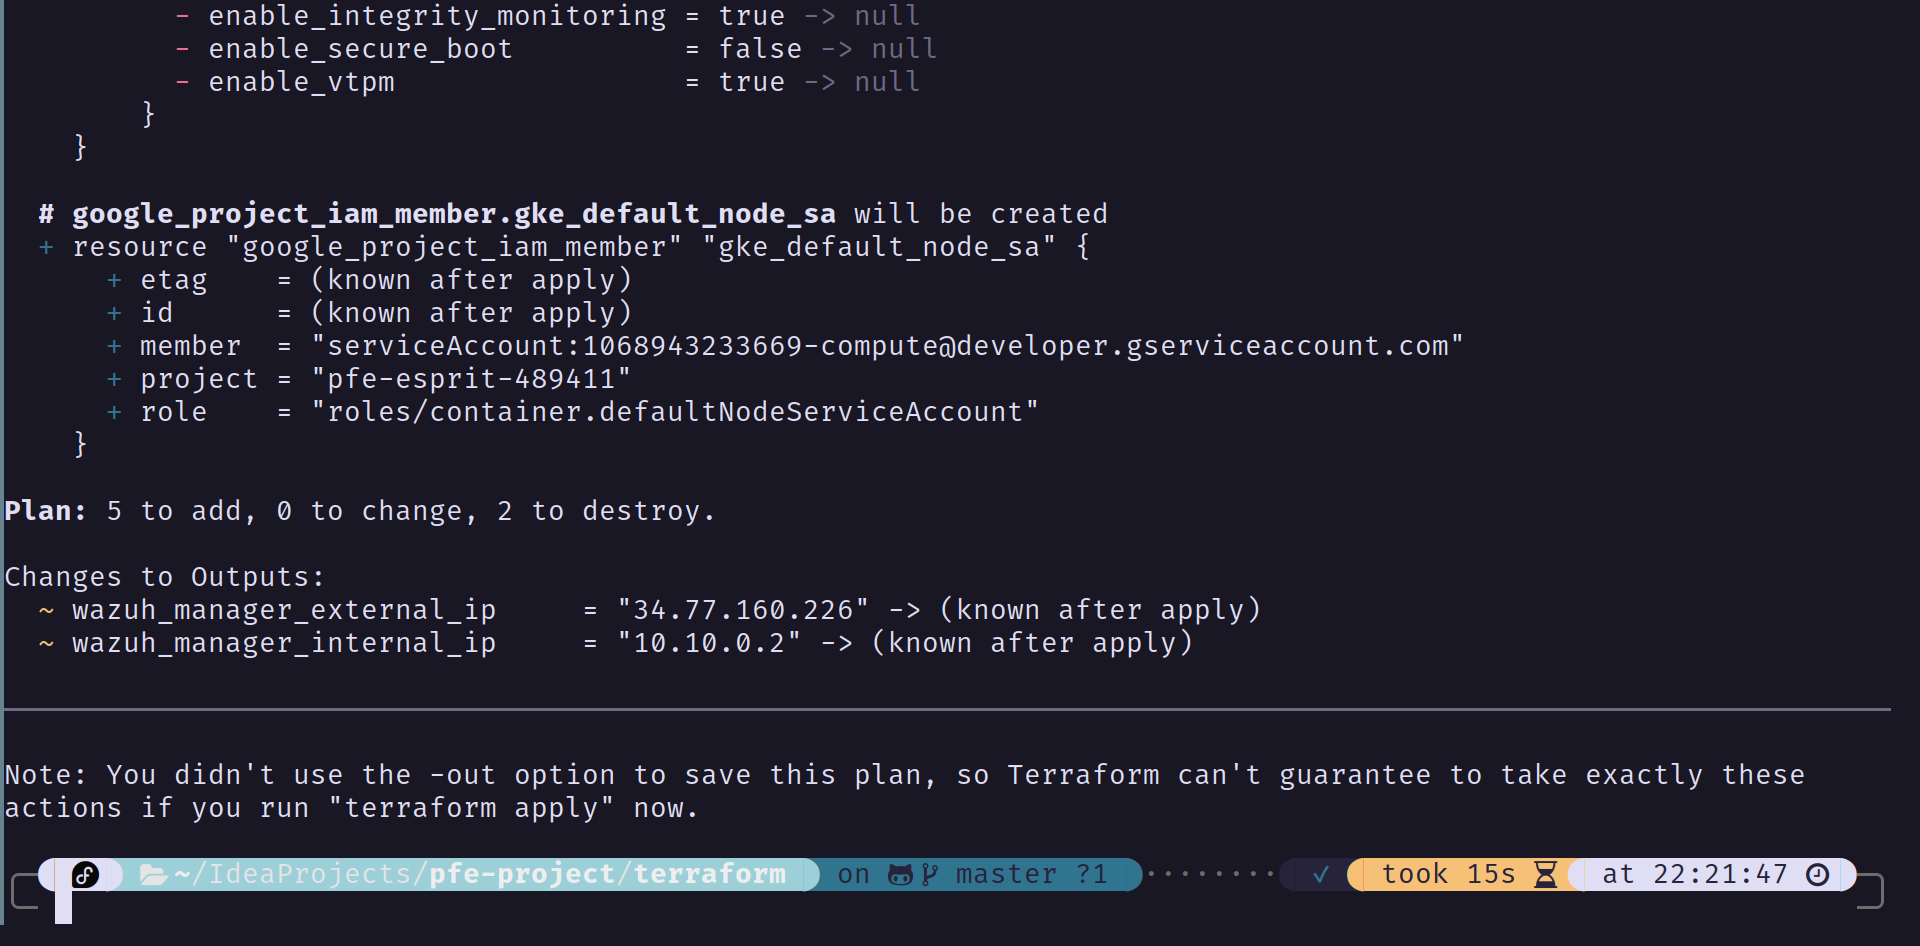
\includegraphics[width=0.95\textwidth,keepaspectratio]{images/screenshots/terraform-plan-gke-node-service-account-changes}
    \caption{Sortie de \texttt{terraform plan} montrant les changements sur le service account GKE}
    \label{fig:terraform_plan}
\end{figure}

\begin{figure}[H]
    \centering
    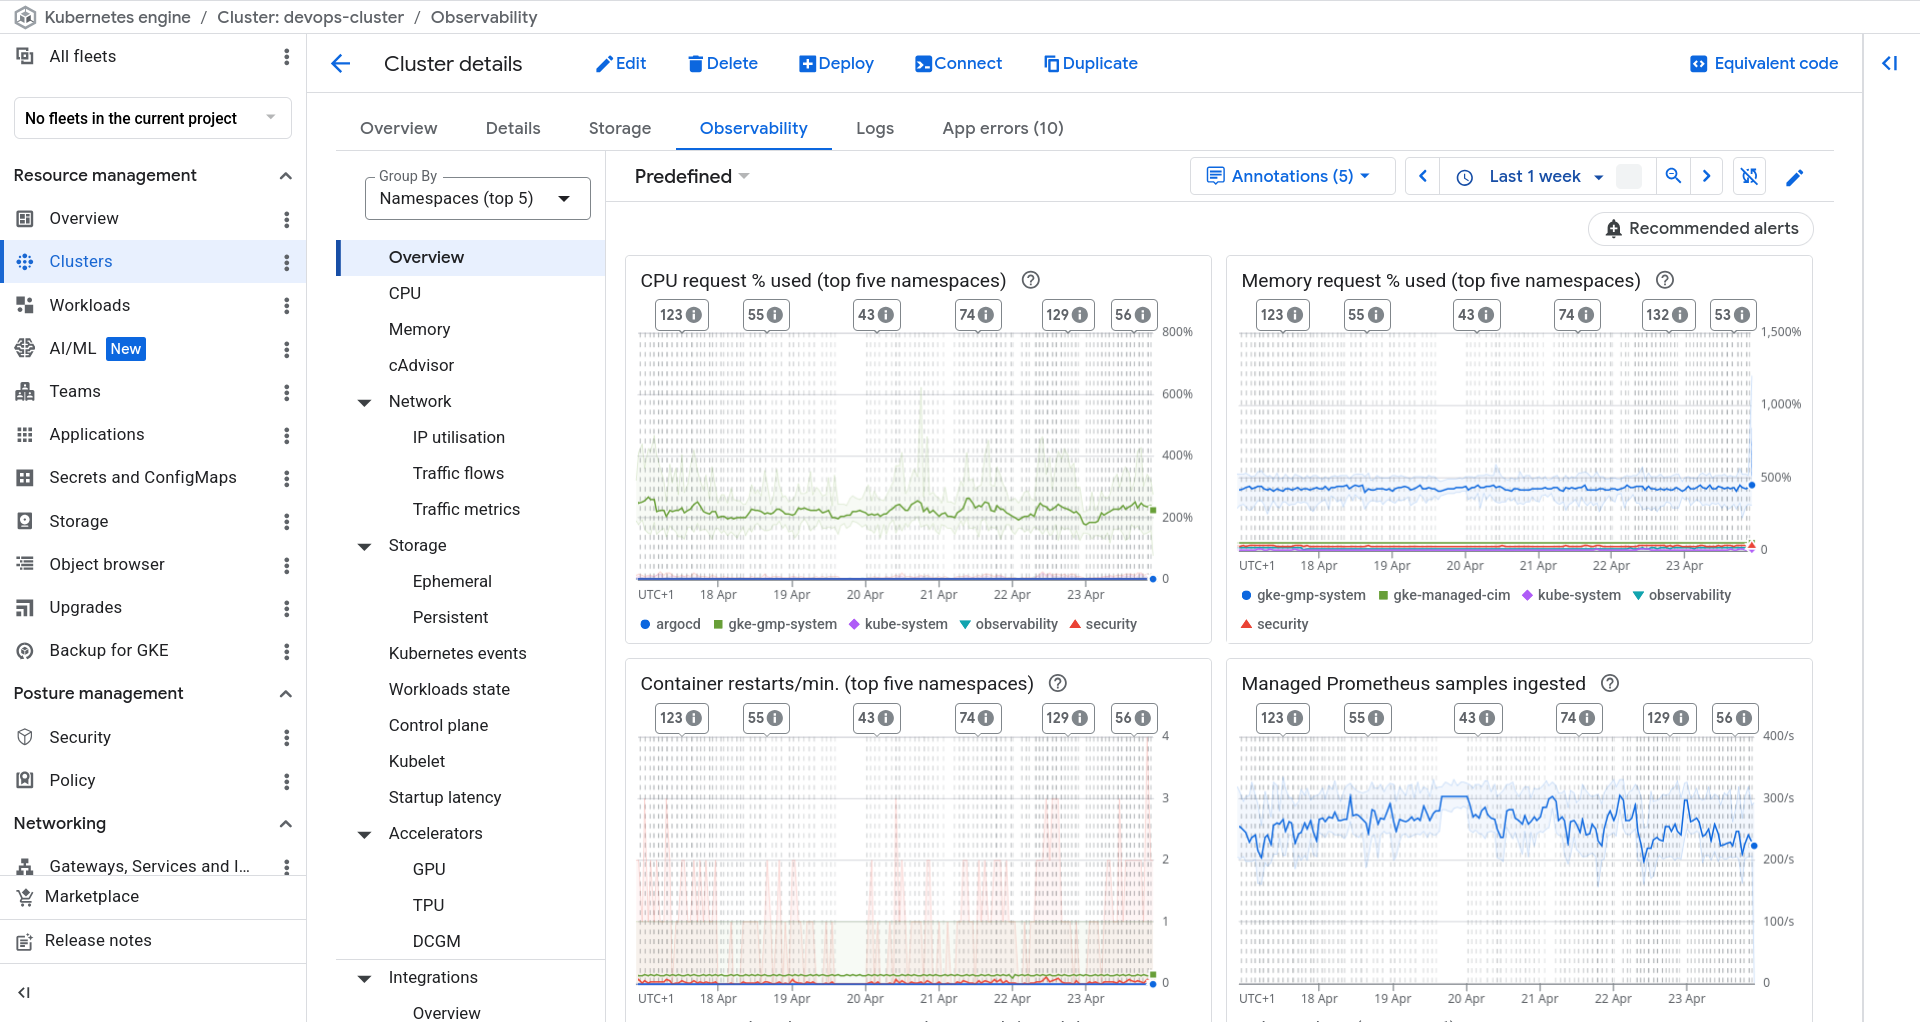
\includegraphics[width=0.95\textwidth,keepaspectratio]{images/screenshots/gke-cluster-observability-dashboard}
    \caption{Dashboard du cluster GKE Autopilot dans la console GCP}
    \label{fig:gke_console}
\end{figure}

\subsection{Rétrospective Sprint 1}

\begin{table}[H]
\centering
\setlength{\arrayrulewidth}{0.8pt}
\renewcommand{\arraystretch}{1.4}
\caption{Rétrospective Sprint 1}
\label{tab:retro_s1}
\begin{tabularx}{\textwidth}{|>{\centering\arraybackslash}X|X|}
\hline
\tableheader \textbf{Catégorie} & \textbf{Détail} \\
\hline
Ce qui a bien marché & Infrastructure 100\% reproductible, Terraform plan clair \\
\hline
Difficultés & Configuration initiale du WIF provider, activation séquentielle des APIs GCP \\
\hline
Livrable & Cluster GKE + VPC + IAM + VM Wazuh opérationnels \\
\hline
\end{tabularx}
\end{table}


%% ================================================================
%%  SPRINT 2 — Containerisation et Pipeline CI/CD
%% ================================================================
\section{Sprint 2~: Containerisation et Pipeline CI/CD}

\subsection{Objectif et Backlog du Sprint}

\begin{table}[H]
\centering
\setlength{\arrayrulewidth}{0.8pt}
\setlength{\dashlinedash}{3pt}
\setlength{\dashlinegap}{2pt}
\renewcommand{\arraystretch}{1.4}
\caption{Backlog du Sprint 2}
\label{tab:backlog_s2}
\begin{tabularx}{\textwidth}{|>{\centering\arraybackslash}X|>{\centering\arraybackslash}X|>{\centering\arraybackslash}X|}
\hline
\tableheader \textbf{User Story} & \textbf{Tâche} & \textbf{Statut} \\
\hline
US-03~: Dockerfile multi-stage & Écrire le Dockerfile avec build Bun + runner Nginx & Terminé \\ \hdashline
US-03 & Introduire les vulnérabilités intentionnelles (nginx:1.21, secrets ENV) & Terminé \\ \hdashline
US-04~: Pipeline CI & Configurer GitHub Actions (build-test, app-image-release) & Terminé \\ \hdashline
US-05~: Auth Keyless (WIF) & Configurer l'authentification OIDC dans le pipeline & Terminé \\ \hdashline
US-04 & Configurer le job update-k8s-tags & Terminé \\
\hline
\end{tabularx}
\end{table}

\subsection{Containerisation et Sécurité des Images Docker}

\subsubsection{Build Multi-Étapes}

Le \texttt{Dockerfile} utilise un \textbf{build multi-étapes} pour minimiser la taille
de l'image finale et réduire la surface d'attaque~:

\begin{lstlisting}[language=bash, caption=Dockerfile multi-étapes (version vulnérable pour démo)]
# Stage 1 : Build avec Bun
FROM oven/bun:1 AS builder
WORKDIR /app
COPY package.json bun.lock ./
RUN bun install
COPY . .
RUN bun run build
# --> dist/ contient les assets statiques compiles
# Stage 2 : Serveur Nginx minimal
FROM nginx:1.21 AS runner   # Attention : version vulnerable (demo)
COPY --from=builder /app/dist /usr/share/nginx/html
COPY ./nginx.conf /etc/nginx/conf.d/default.conf
EXPOSE 80
CMD ["nginx", "-g", "daemon off;"]
\end{lstlisting}

\subsubsection{Vulnérabilités Intentionnelles dans le Dockerfile}

\begin{table}[H]
\centering
\setlength{\arrayrulewidth}{0.8pt}
\setlength{\dashlinedash}{3pt}
\setlength{\dashlinegap}{2pt}
\renewcommand{\arraystretch}{1.4}
\caption{Vulnérabilités intentionnelles dans le Dockerfile}
\label{tab:dockerfile_vulns}
\begin{tabularx}{\textwidth}{|>{\centering\arraybackslash}X|>{\centering\arraybackslash}X|>{\centering\arraybackslash}X|>{\centering\arraybackslash}X|}
\hline
\tableheader \textbf{Vulnérabilité} & \textbf{Ligne} & \textbf{Outil} & \textbf{Sévérité} \\
\hline
Image nginx obsolète (CVEs OS) & \texttt{FROM nginx:1.21} & Trivy & CRITICAL/HIGH \\ \hdashline
Secrets hardcodés en ENV & \texttt{ENV APP\_SECRET=...} & Trivy & HIGH \\ \hdashline
Fichier .env copié dans l'image & \texttt{COPY .env ...} & Trivy & HIGH \\ \hdashline
Exécution en root (pas de USER) & Absent & Trivy DS002 & MEDIUM \\ \hdashline
Pas de HEALTHCHECK & Absent & Trivy DS026 & LOW \\
\hline
\end{tabularx}
\end{table}

\subsubsection{Comparaison Image Vulnérable vs Durcie}

\begin{table}[H]
\centering
\setlength{\arrayrulewidth}{0.8pt}
\setlength{\dashlinedash}{3pt}
\setlength{\dashlinegap}{2pt}
\renewcommand{\arraystretch}{1.4}
\caption{nginx:1.21 vs nginx:alpine}
\label{tab:nginx_compare}
\begin{tabularx}{\textwidth}{|>{\centering\arraybackslash}X|>{\centering\arraybackslash}X|>{\centering\arraybackslash}X|}
\hline
\tableheader \textbf{Aspect} & \textbf{nginx:1.21 (vulnérable)} & \textbf{nginx:alpine (durci)} \\
\hline
CVEs OS critiques & Plusieurs dizaines & Quasi-inexistants \\ \hdashline
Taille image & $\sim$133 MB & $\sim$23 MB \\ \hdashline
Utilisateur & root & non-root possible \\ \hdashline
Surface d'attaque & Large & Minimale \\
\hline
\end{tabularx}
\end{table}

\subsection{Pipeline CI/CD avec GitHub Actions}

\subsubsection{Vue Globale du Pipeline}

Le pipeline GitHub Actions est déclenché à chaque \textit{push} sur la branche principale.
Il s'articule en plusieurs jobs interdépendants~:
\begin{enumerate}
  \item \textbf{build-test}~: tests unitaires, lint, SonarCloud, Trivy FS~;
  \item \textbf{prepare-release-infra}~: parallèle app-image-release et playwright-release~;
  \item \textbf{app-image-release}~: build image Docker, push vers Artifact Registry, scan Trivy~;
  \item \textbf{update-k8s-tags}~: commit du nouveau SHA dans les manifests Kubernetes~;
  \item \textbf{e2e-tests}~: matrice de 6 jobs Playwright (@t1 à @t6)~;
  \item \textbf{zap-baseline}~: scan DAST OWASP ZAP post-déploiement.
\end{enumerate}

\begin{figure}[H]
    \centering
    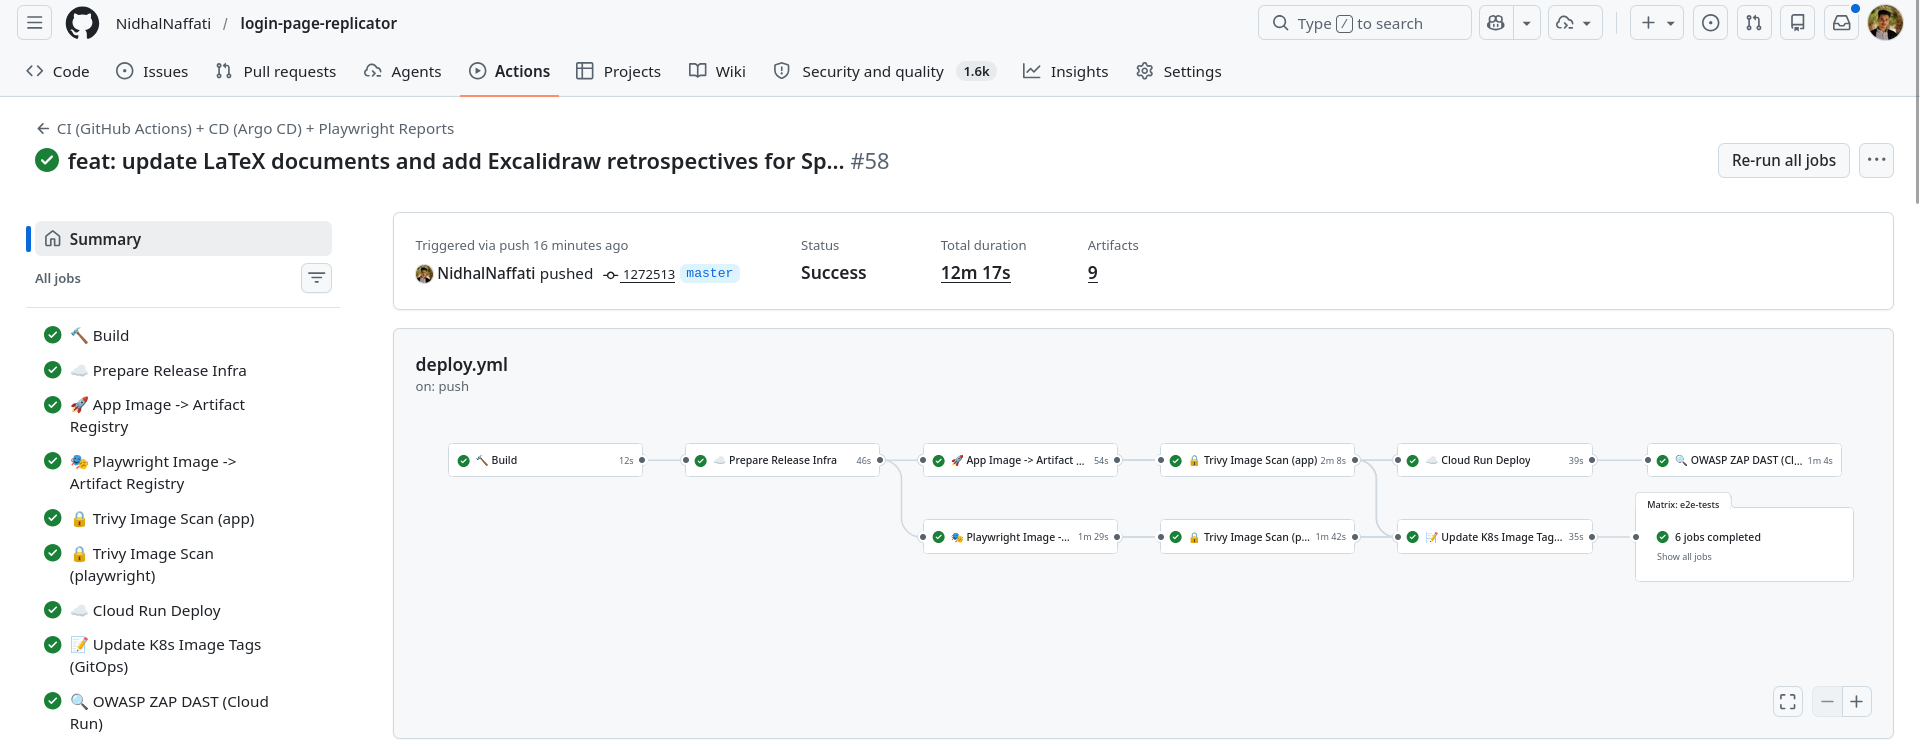
\includegraphics[width=0.95\textwidth,keepaspectratio]{images/screenshots/github-actions-ci-cd-workflow-summary}
    \caption{Vue globale du pipeline CI/CD dans GitHub Actions}
    \label{fig:pipeline_overview}
\end{figure}

\subsubsection{Job build-test --- Première Ligne de Défense}

Le job \texttt{build-test} constitue la premiere ligne de defense securitaire~:
\begin{lstlisting}[language=bash, caption=Extrait du job build-test GitHub Actions]
build-test:
  runs-on: ubuntu-latest
  steps:
    - uses: actions/checkout@v4
    - uses: oven-sh/setup-bun@v2
    - run: bun install
    - run: bun run lint
    - run: bun run test:coverage
    - name: SonarCloud Scan
      uses: SonarSource/sonarcloud-github-action@master
      env:
        SONAR_TOKEN: ${{ secrets.SONAR_TOKEN }}
    - name: Trivy FS Scan
      uses: aquasecurity/trivy-action@master
      with:
        scan-type: 'fs'
        format: 'sarif'
        output: 'trivy-fs-results.sarif'
        scanners: 'vuln,secret,misconfig'
    - uses: github/codeql-action/upload-sarif@v3
      with:
        sarif_file: 'trivy-fs-results.sarif'
\end{lstlisting}
\subsubsection{Authentification sans Clés Statiques --- Workload Identity Federation}
L'un des apports majeurs de ce projet est le remplacement des clés JSON statiques par
l'authentification \textbf{OIDC via Workload Identity Federation}~:
\begin{lstlisting}[language=bash, caption=Authentification GCP sans clé statique]
# Avant : secrets.GCP_SA_KEY (cle JSON longue duree)
# Apres :
- name: Authenticate to GCP via WIF
  uses: google-github-actions/auth@v2
  with:
    workload_identity_provider: ${{ secrets.WIF_PROVIDER }}
    service_account: ${{ secrets.WIF_SERVICE_ACCOUNT }}
\end{lstlisting}
GitHub Actions obtient un \textbf{token OIDC éphémère} valide 1 heure maximum, échangé
contre des credentials GCP temporaires. Aucune clé persistante n'est stockée.
\begin{figure}[H]
    \centering
    \fbox{\parbox{0.85\textwidth}{\centering
        \vspace{2.5cm}
        Espace réservé pour la Figure~\ref{fig:build_test_screenshot}\\
        \textbf{Capture d'écran~: Job build-test réussi dans GitHub Actions}
        \vspace{2.5cm}
    }}
    \caption{Exécution réussie du job build-test}
    \label{fig:build_test_screenshot}
\end{figure}
\subsection{Orchestration Kubernetes sur GKE}
Le déploiement définit \textbf{deux containers dans le même pod}~:
\begin{itemize}
  \item \textbf{Container \texttt{app}}~: image Nginx servant l'application React compilée,
        port 80, ressources \texttt{cpu: 100m}, \texttt{memory: 128Mi}~;
  \item \textbf{Container \texttt{nginx-exporter}} (sidecar)~: image
        \texttt{nginx/nginx-prometheus-exporter:1.1.0}, expose les métriques Nginx en format
        Prometheus sur le port 9113.
\end{itemize}
L'HPA maintient \textbf{2 replicas minimum} et scale jusqu'à \textbf{8 replicas} à 60\%
d'utilisation CPU. Un Ingress GCE expose l'application sur Internet.
\subsection{Rétrospective Sprint 2}

\begin{table}[H]
\centering
\setlength{\arrayrulewidth}{0.8pt}
\renewcommand{\arraystretch}{1.4}
\caption{Rétrospective Sprint 2}
\label{tab:retro_s2}
\begin{tabularx}{\textwidth}{|>{\centering\arraybackslash}X|X|}
\hline
\tableheader \textbf{Catégorie} & \textbf{Détail} \\
\hline
Ce qui a bien marché & Pipeline CI fonctionnel dès le premier push, WIF opérationnel \\
\hline
Difficultés & Configuration OIDC WIF (concepts peu documentés), orchestration des jobs GitHub Actions \\
\hline
Livrable & Pipeline CI/CD complet, image Docker publiée, app déployée sur GKE \\
\hline
\end{tabularx}
\end{table}


%% ================================================================
%%  SPRINT 3 — Sécurité Intégrée et GitOps
%% ================================================================
\section{Sprint 3~: Sécurité Intégrée et GitOps}

\subsection{Objectif et Backlog du Sprint}

\begin{table}[H]
\centering
\setlength{\arrayrulewidth}{0.8pt}
\setlength{\dashlinedash}{3pt}
\setlength{\dashlinegap}{2pt}
\renewcommand{\arraystretch}{1.4}
\caption{Backlog du Sprint 3}
\label{tab:backlog_s3}
\begin{tabularx}{\textwidth}{|>{\centering\arraybackslash}X|>{\centering\arraybackslash}X|>{\centering\arraybackslash}X|}
\hline
\tableheader \textbf{User Story} & \textbf{Tâche} & \textbf{Statut} \\
\hline
US-06~: Scans SAST/SCA & Intégrer SonarCloud et Trivy (3 niveaux) dans le pipeline & Terminé \\ \hdashline
US-07~: GitOps Argo CD & Configurer l'Application Argo CD avec auto-sync et self-heal & Terminé \\ \hdashline
US-07 & Configurer les PostSync hooks pour Playwright & Terminé \\ \hdashline
US-08~: Zero Trust & Créer les 12 NetworkPolicies default-deny & Terminé \\ \hdashline
US-09~: DAST ZAP & Intégrer le scan OWASP ZAP baseline post-déploiement & Terminé \\
\hline
\end{tabularx}
\end{table}

\subsection{SAST avec SonarCloud}

SonarCloud analyse le code TypeScript/React à chaque push et détecte~:
\begin{itemize}
  \item \textbf{Security Hotspots}~: utilisations de \texttt{dangerouslySetInnerHTML} (XSS)~;
  \item \textbf{Vulnerabilities}~: patterns de code pouvant mener à des injections~;
  \item \textbf{Code Smells}~: indicateurs de qualité masquant des vulnérabilités~;
  \item \textbf{Coverage gate}~: bloque la PR si la couverture de tests chute sous le seuil.
\end{itemize}

\begin{figure}[H]
    \centering
    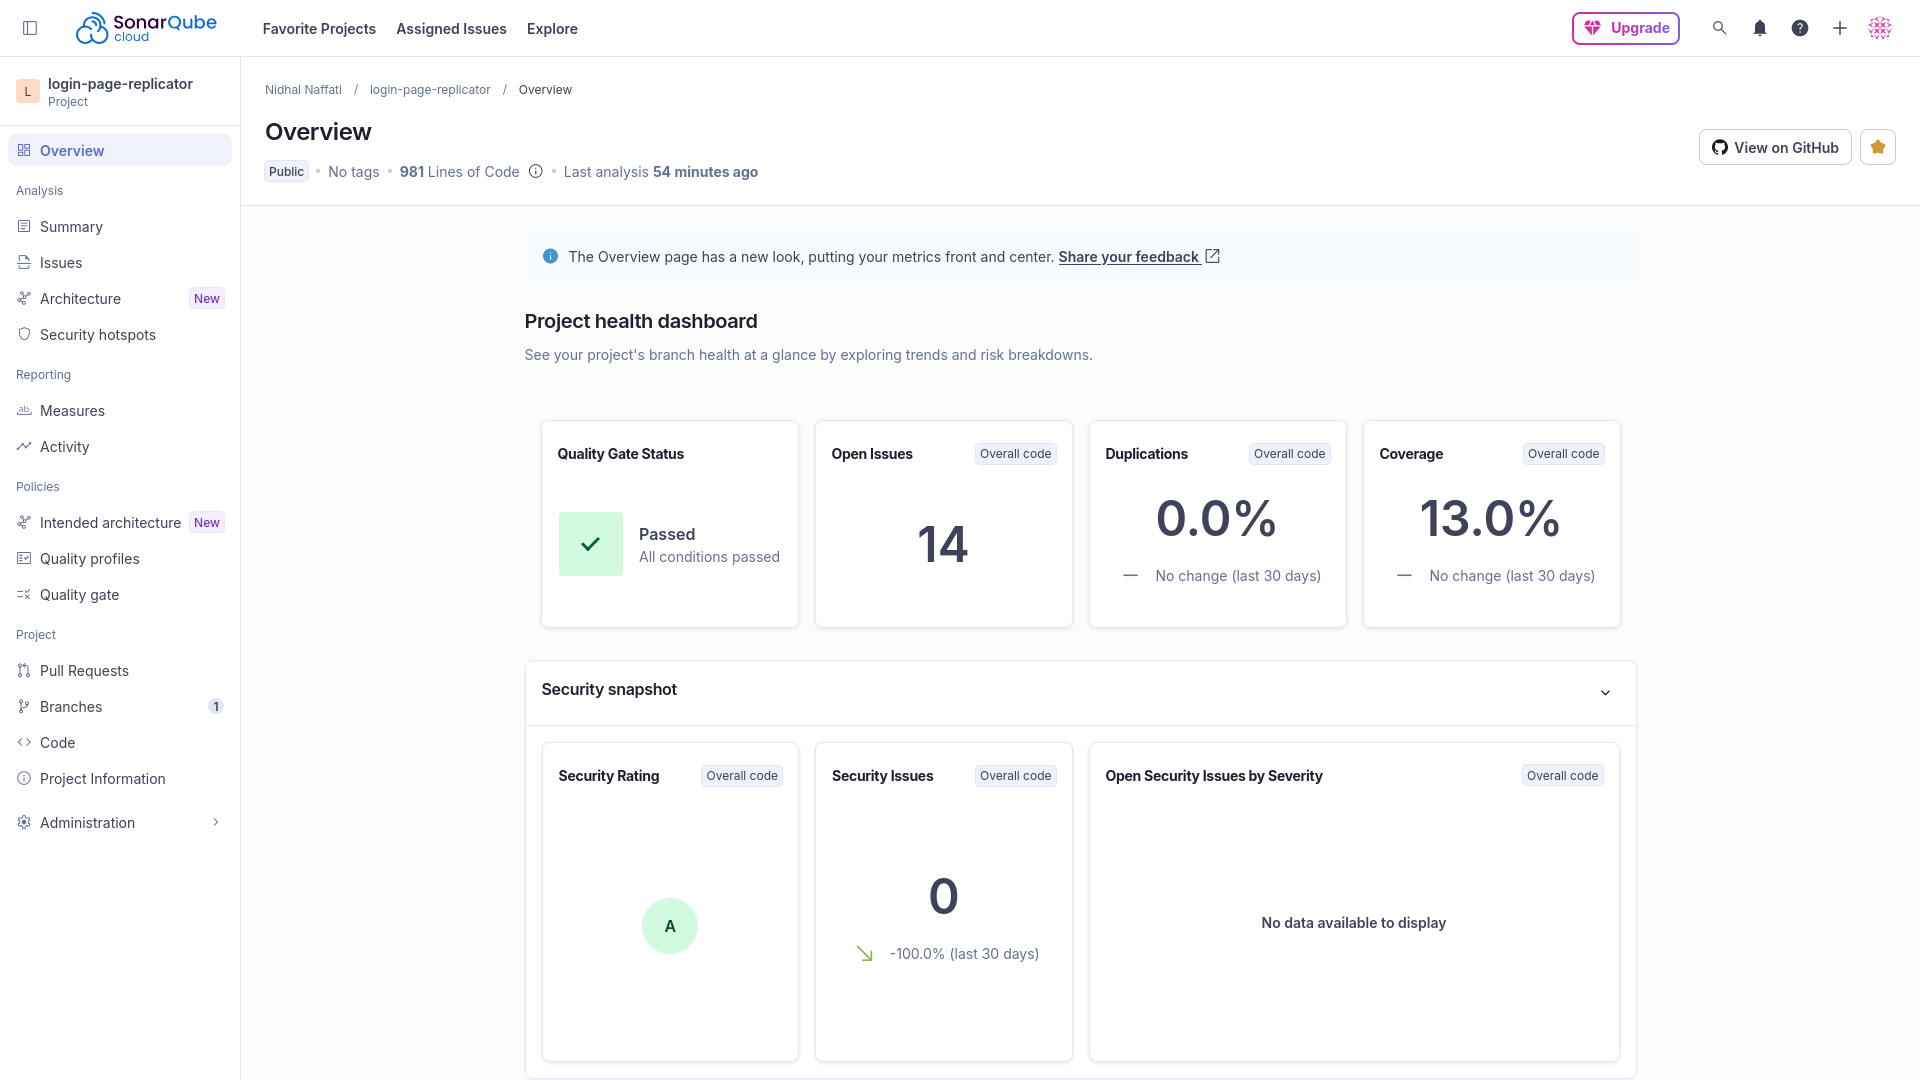
\includegraphics[width=0.95\textwidth,keepaspectratio]{images/screenshots/sonarqube-overview-dashboard}
    \caption{Dashboard SonarCloud montrant la vue d'ensemble du projet}
    \label{fig:sonarcloud_dashboard}
\end{figure}

\begin{figure}[H]
    \centering
    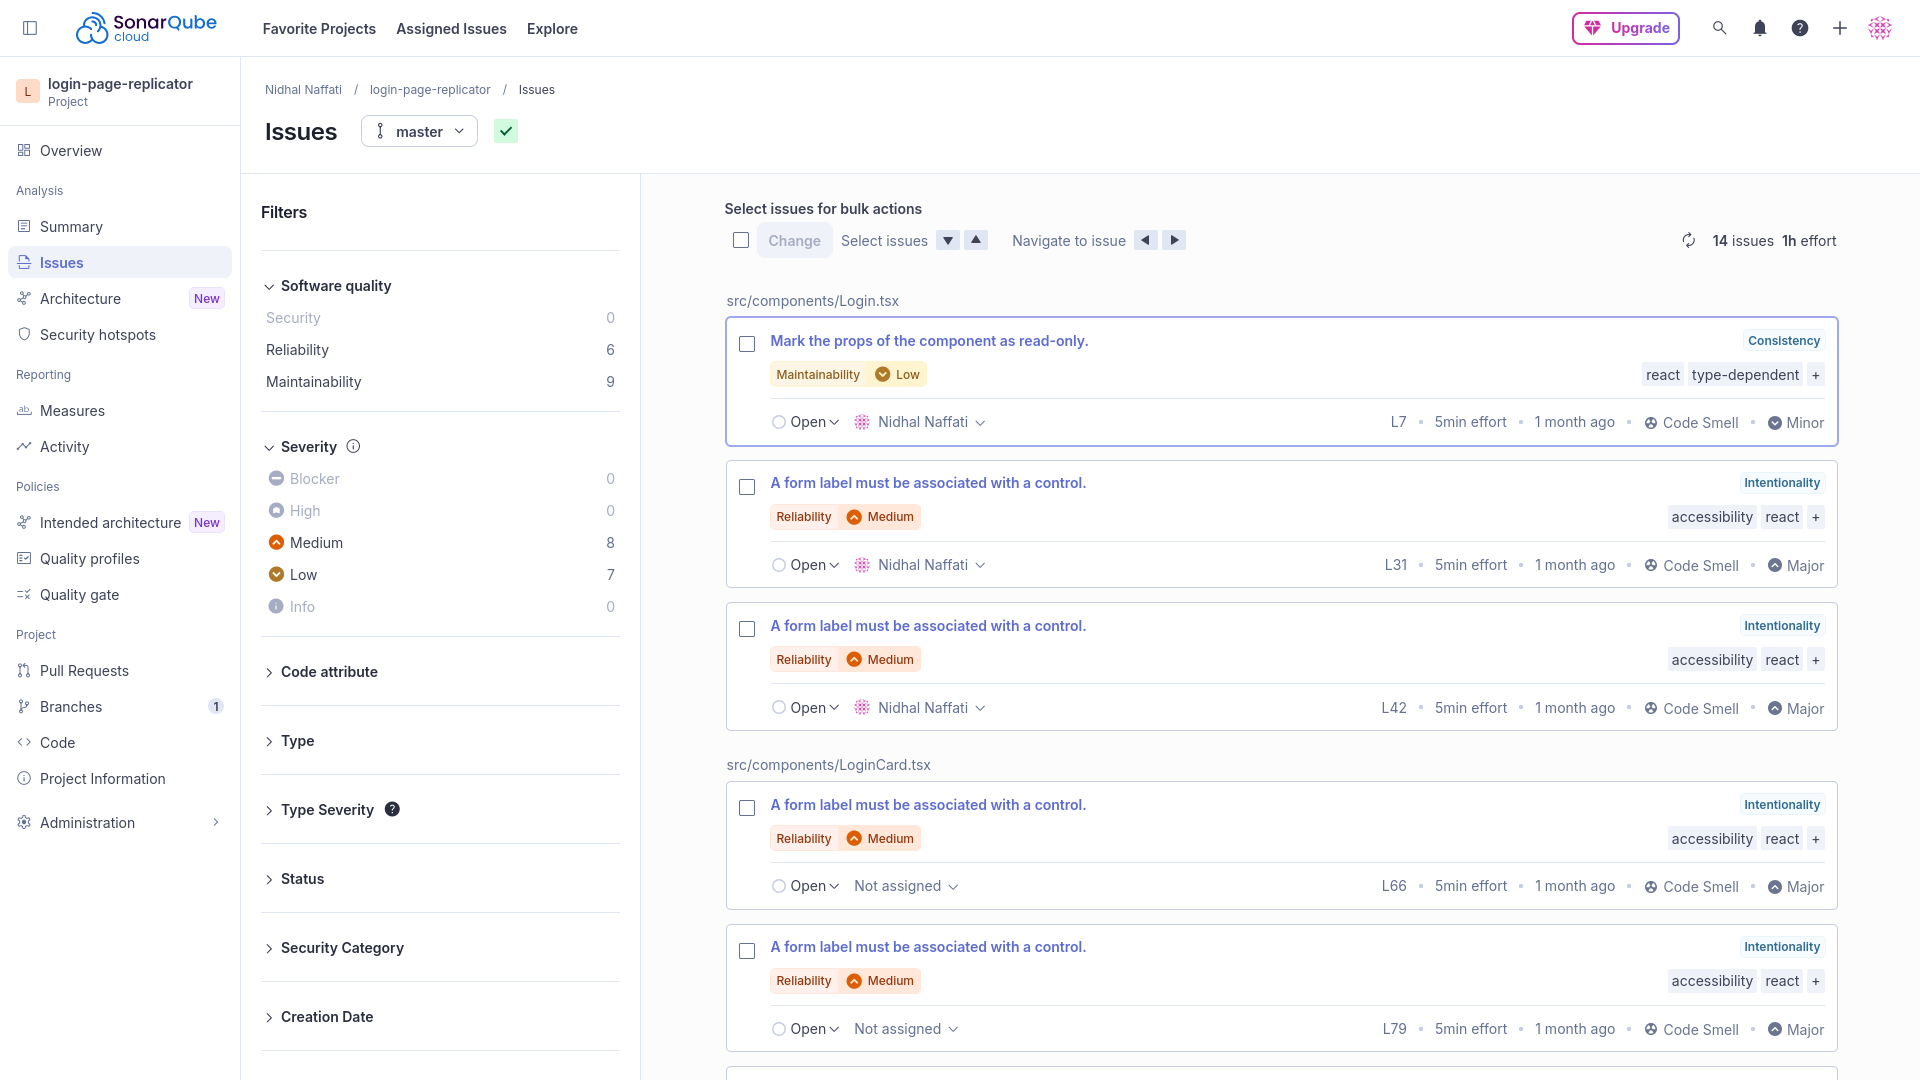
\includegraphics[width=0.95\textwidth,keepaspectratio]{images/screenshots/sonarqube-issues-list}
    \caption{Liste des issues de sécurité détectées par SonarCloud}
    \label{fig:sonarcloud_issues}
\end{figure}

\subsection{SCA avec Trivy --- Vulnérabilités Détectées}

Le tableau~\ref{tab:trivy_scans} détaille les trois niveaux de scan Trivy intégrés~:

\begin{table}[H]
\centering
\setlength{\arrayrulewidth}{0.8pt}
\setlength{\dashlinedash}{3pt}
\setlength{\dashlinegap}{2pt}
\renewcommand{\arraystretch}{1.4}
\caption{Les trois niveaux de scan Trivy dans le pipeline}
\label{tab:trivy_scans}
\begin{tabularx}{\textwidth}{|>{\centering\arraybackslash}X|>{\centering\arraybackslash}X|>{\centering\arraybackslash}X|}
\hline
\tableheader \textbf{Scan} & \textbf{Cible} & \textbf{Ce qui est détecté} \\
\hline
\texttt{trivy fs} & Code source + \texttt{package.json} & Vulns deps npm, secrets dans fichiers \\ \hdashline
\texttt{trivy image} & Image Docker construite & CVEs OS, secrets ENV \\ \hdashline
\texttt{trivy config} & Manifests YAML Kubernetes & Misconfigurations IaC \\
\hline
\end{tabularx}
\end{table}

\begin{table}[H]
\centering
\setlength{\arrayrulewidth}{0.8pt}
\setlength{\dashlinedash}{3pt}
\setlength{\dashlinegap}{2pt}
\renewcommand{\arraystretch}{1.4}
\caption{CVEs détectées par Trivy FS sur les dépendances npm}
\label{tab:cves_npm}
\begin{tabularx}{\textwidth}{|>{\centering\arraybackslash}X|>{\centering\arraybackslash}X|>{\centering\arraybackslash}X|>{\centering\arraybackslash}X|}
\hline
\tableheader \textbf{CVE} & \textbf{Package} & \textbf{Sévérité} & \textbf{Description} \\
\hline
CVE-2021-23337 & lodash 4.17.20 & HIGH & Command Injection \\ \hdashline
CVE-2026-4800  & lodash 4.17.20 & HIGH & Code Injection via \_.template \\ \hdashline
CVE-2025-13465 & lodash 4.17.20 & MEDIUM & Prototype Pollution \\ \hdashline
CVE-2022-23539 & jsonwebtoken 8.5.1 & HIGH & Insecure key types \\ \hdashline
CVE-2022-23540 & jsonwebtoken 8.5.1 & MEDIUM & Signature bypass (none algo) \\ \hdashline
CVE-2022-23541 & jsonwebtoken 8.5.1 & MEDIUM & RSA to HMAC forgery \\ \hdashline
CVE-2024-29041 & express 4.17.1 & MEDIUM & Open Redirect \\
\hline
\end{tabularx}
\end{table}

Le scan de l'image \texttt{nginx:1.21} révèle \textbf{47 vulnérabilités}~: 3 CRITICAL, 12 HIGH,
18 MEDIUM, 14 LOW.

\begin{figure}[H]
    \centering
    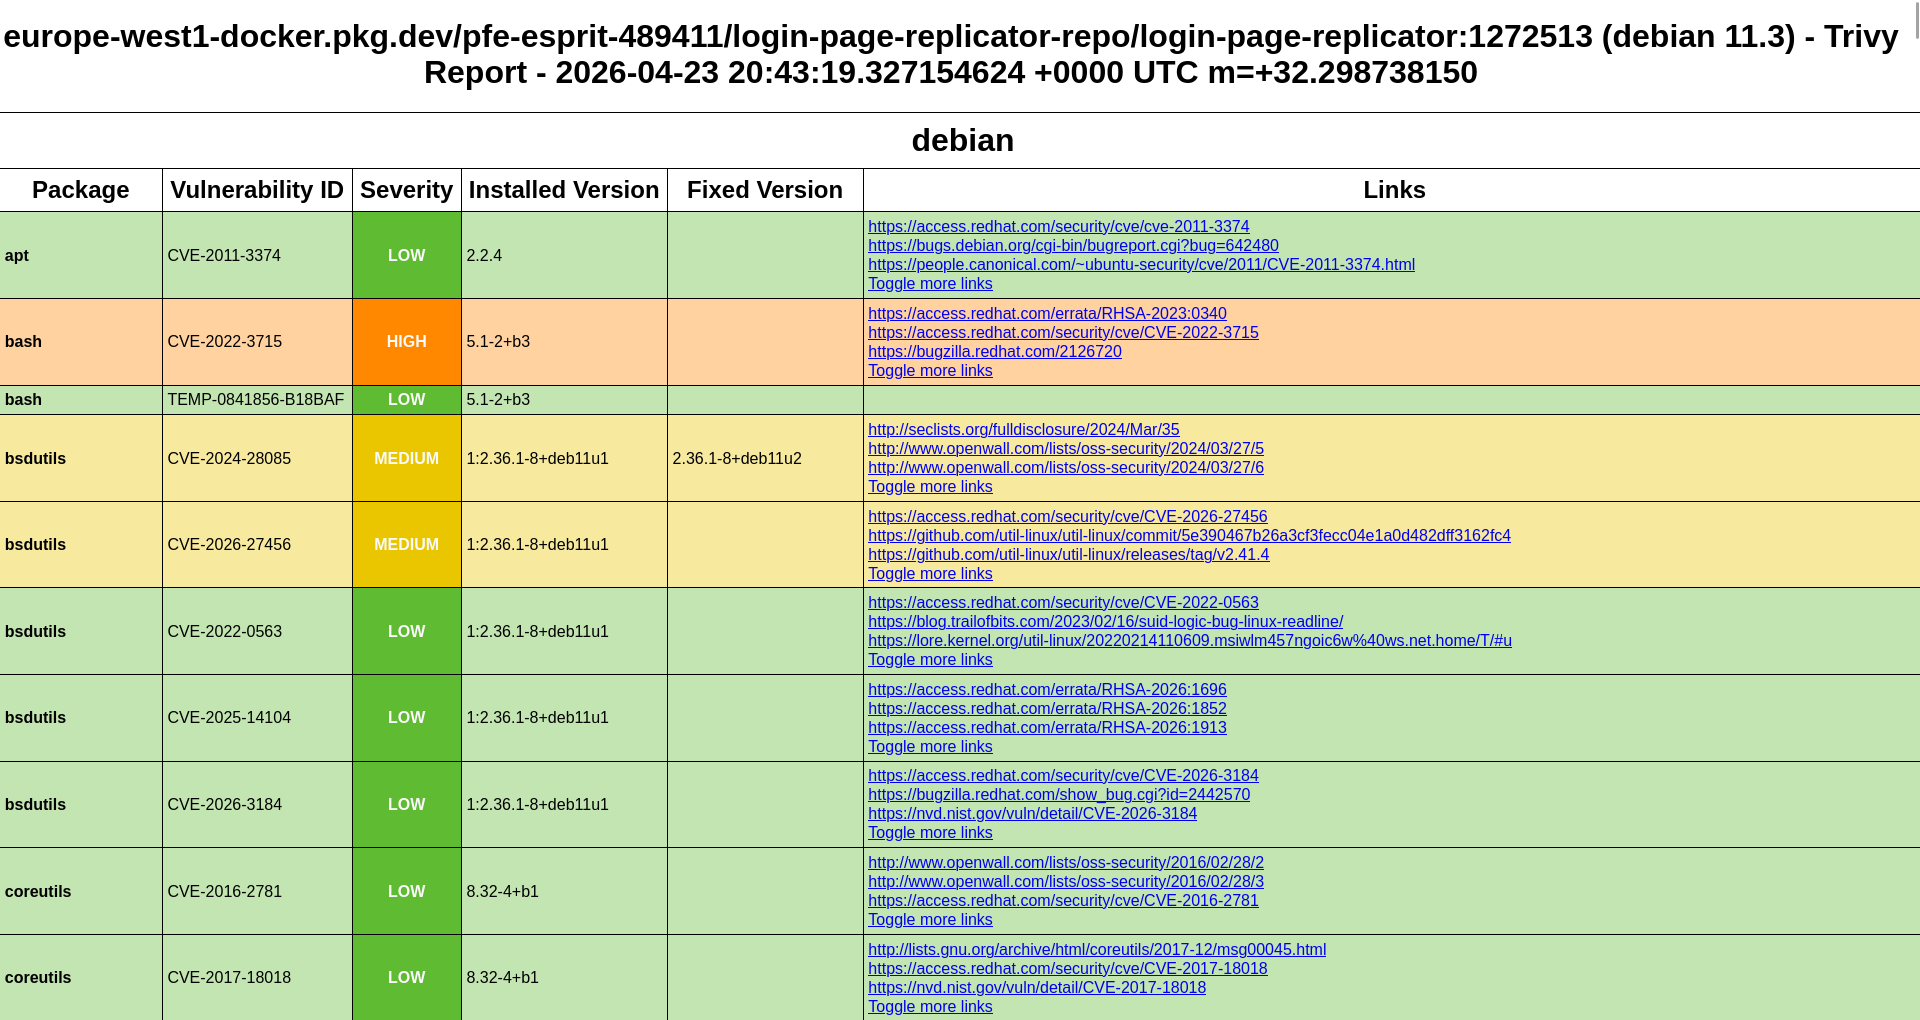
\includegraphics[width=0.95\textwidth,keepaspectratio]{images/screenshots/trivy-debian-vulnerability-report-overview}
    \caption{Vue d'ensemble du rapport Trivy sur l'image nginx:1.21 (Debian)}
    \label{fig:trivy_scan_results}
\end{figure}

\begin{figure}[H]
    \centering
    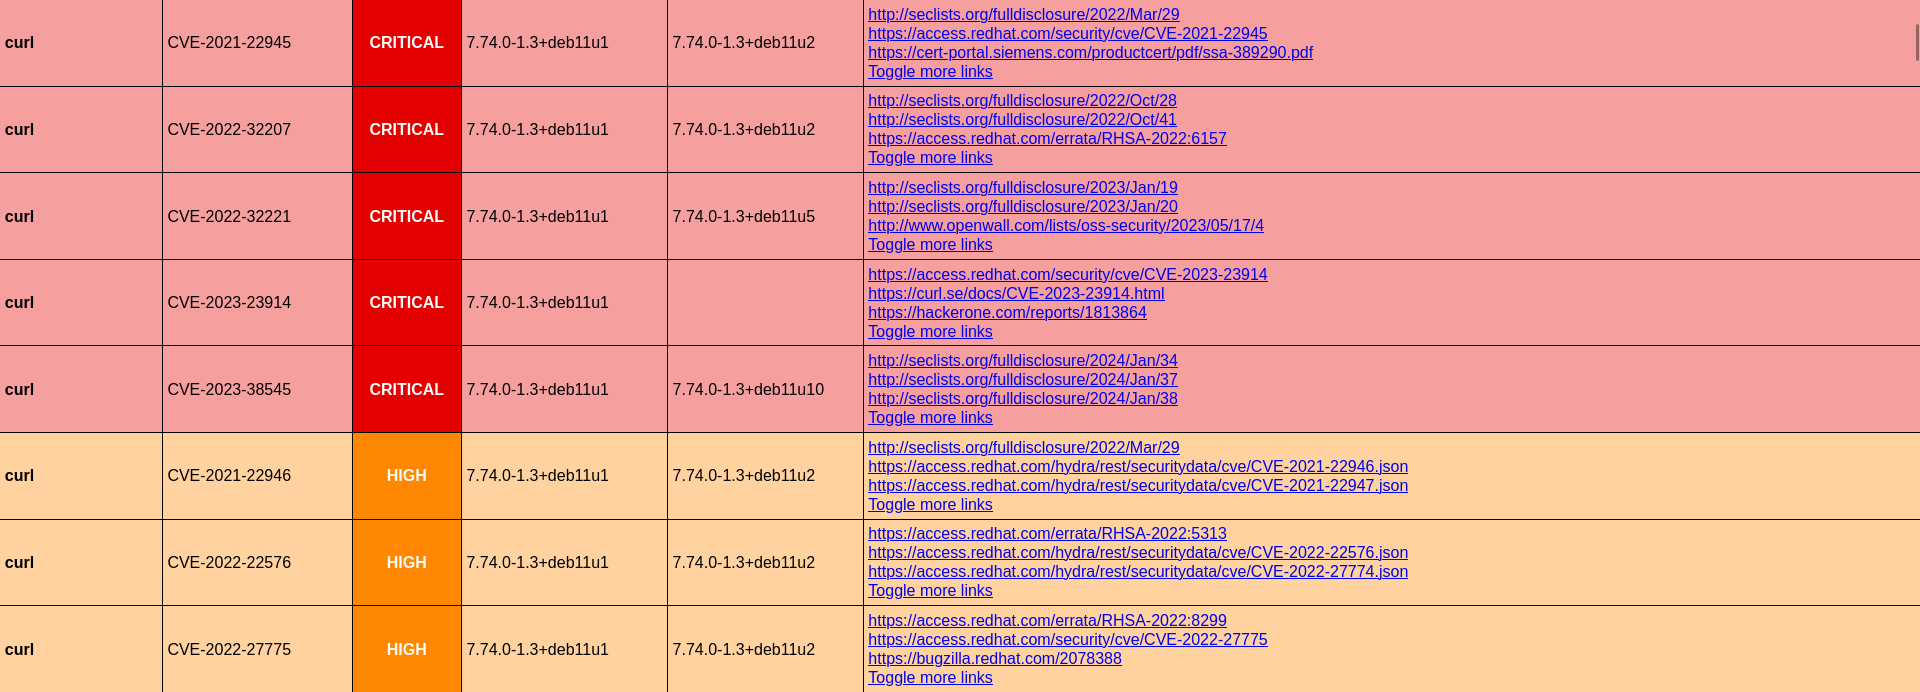
\includegraphics[width=0.95\textwidth,keepaspectratio]{images/screenshots/trivy-debian-curl-critical-vulnerabilities}
    \caption{Détail des vulnérabilités critiques détectées par Trivy (curl/libcurl)}
    \label{fig:trivy_critical_detail}
\end{figure}

\subsection{DAST avec OWASP ZAP}

OWASP ZAP effectue un scan en boîte noire de l'application déployée~:

\begin{table}[H]
\centering
\setlength{\arrayrulewidth}{0.8pt}
\setlength{\dashlinedash}{3pt}
\setlength{\dashlinegap}{2pt}
\renewcommand{\arraystretch}{1.4}
\caption{Findings OWASP ZAP sur l'application}
\label{tab:zap_findings}
\begin{tabularx}{\textwidth}{|>{\centering\arraybackslash}X|>{\centering\arraybackslash}X|>{\centering\arraybackslash}X|}
\hline
\tableheader \textbf{Finding} & \textbf{Règle} & \textbf{Sévérité} \\
\hline
Stored XSS (dangerouslySetInnerHTML) & 40012 & HIGH \\ \hdashline
Missing Content-Security-Policy & 10038 & MEDIUM \\ \hdashline
Missing X-Frame-Options (Clickjacking) & 10020 & MEDIUM \\ \hdashline
Directory Browsing Enabled & 10033 & MEDIUM \\ \hdashline
Cookie sans flag Secure & 10011 & LOW \\ \hdashline
Cookie sans flag HttpOnly & 10010 & LOW \\ \hdashline
CORS Wildcard (*) & --- & LOW \\ \hdashline
Server Version Leaked (nginx/1.21.6) & 10036 & LOW \\ \hdashline
Missing HSTS & 10035 & LOW \\ \hdashline
Missing X-Content-Type-Options & 10021 & LOW \\
\hline
\end{tabularx}
\end{table}

Après durcissement de \texttt{nginx.conf} (ajout des headers de sécurité, désactivation de
\texttt{server\_tokens} et \texttt{autoindex})~: \textbf{0 FAIL, 0 WARN}.

\subsubsection{Comparaison nginx.conf Vulnérable vs Durci}

\begin{table}[H]
\centering
\setlength{\arrayrulewidth}{0.8pt}
\setlength{\dashlinedash}{3pt}
\setlength{\dashlinegap}{2pt}
\renewcommand{\arraystretch}{1.4}
\caption{Comparaison de la configuration nginx avant et après durcissement}
\label{tab:nginx_harden}
\begin{tabularx}{\textwidth}{|>{\centering\arraybackslash}X|>{\centering\arraybackslash}X|>{\centering\arraybackslash}X|}
\hline
\tableheader \textbf{Directive} & \textbf{Vulnérable} & \textbf{Durci} \\
\hline
\texttt{server\_tokens} & \texttt{on} & \texttt{off} \\ \hdashline
\texttt{X-Powered-By} & \texttt{Nginx/1.21 + React 18} & Absent \\ \hdashline
\texttt{Content-Security-Policy} & Absent & \texttt{default-src 'self'} \\ \hdashline
\texttt{X-Frame-Options} & Absent & \texttt{DENY} \\ \hdashline
\texttt{X-Content-Type-Options} & Absent & \texttt{nosniff} \\ \hdashline
\texttt{Strict-Transport-Security} & Absent & \texttt{max-age=31536000} \\ \hdashline
\texttt{autoindex} & \texttt{on} & \texttt{off} \\ \hdashline
\texttt{Access-Control-Allow-Origin} & \texttt{*} & Absent ou domaine spécifique \\ \hdashline
\texttt{Set-Cookie} flags & Aucun flag & \texttt{Secure; HttpOnly; SameSite=Strict} \\
\hline
\end{tabularx}
\end{table}

\subsubsection{Démonstration des Vulnérabilités Applicatives}

Pour démontrer la pertinence des scanners, l'application contient des \textbf{vulnérabilités
intentionnelles clairement documentées}. Le tableau~\ref{tab:vuln_demo} synthétise les
principales démonstrations réalisables~:

\begin{table}[H]
\centering
\setlength{\arrayrulewidth}{0.8pt}
\setlength{\dashlinedash}{3pt}
\setlength{\dashlinegap}{2pt}
\renewcommand{\arraystretch}{1.4}
\caption{Démonstration des vulnérabilités détectées par les scanners}
\label{tab:vuln_demo}
\begin{tabularx}{\textwidth}{|>{\centering\arraybackslash}X|>{\centering\arraybackslash}X|>{\centering\arraybackslash}X|>{\centering\arraybackslash}X|}
\hline
\tableheader \textbf{Vulnérabilité} & \textbf{CWE} & \textbf{Fichier} & \textbf{Scanner} \\
\hline
XSS stocké (\texttt{dangerouslySetInnerHTML}) & CWE-79 & TodoItem.tsx & SonarCloud + ZAP \\ \hdashline
Open Redirect (\texttt{?redirect=}) & CWE-601 & Login.tsx & SonarCloud \\ \hdashline
Énumération d'utilisateurs & CWE-209 & Login.tsx & SonarCloud \\ \hdashline
Mode debug exposant les credentials & CWE-215 & Login.tsx & SonarCloud \\ \hdashline
Credentials hardcodés (5+ fichiers) & CWE-798 & Multiple & SonarCloud + Trivy \\ \hdashline
Cookies sans Secure/HttpOnly & CWE-614 & Login.tsx, nginx.conf & ZAP \\ \hdashline
\texttt{eval()} injection de code & CWE-95 & TodoDashboard.tsx & SonarCloud \\ \hdashline
Token forgeable (\texttt{Math.random}) & CWE-338 & AuthContext.tsx & SonarCloud \\ \hdashline
Reverse tabnabbing & CWE-1022 & TodoItem.tsx & SonarCloud \\ \hdashline
Données sensibles dans localStorage & CWE-312 & AuthContext.tsx & SonarCloud \\ \hdashline
Credentials loggés en console & CWE-532 & Login.tsx & SonarCloud \\ \hdashline
Duplication de code ($>$5\%) & CWE-1041 & helpers.ts & SonarCloud \\
\hline
\end{tabularx}
\end{table}

\textbf{Exemple de démonstration XSS~:} L'utilisateur saisit
\texttt{<img src=x onerror=alert('XSS')>} comme texte de tâche. Le composant
\texttt{TodoItem} rend ce texte via \texttt{dangerouslySetInnerHTML}, ce qui exécute
le JavaScript et affiche une boîte d'alerte. Cette vulnérabilité est détectée à la fois
par SonarCloud (règle S5247) et par OWASP ZAP (règle 40012).

\begin{figure}[H]
    \centering
    \fbox{\parbox{0.85\textwidth}{\centering
        \vspace{2.5cm}
        Espace réservé pour la Figure~\ref{fig:xss_demo}\\
        \textbf{Capture d'écran~: Démonstration de la vulnérabilité XSS stockée}\\[6pt]
        \footnotesize Payload~: \texttt{<img src=x onerror=alert('XSS')>} $\to$ alert box affichée
        \vspace{2.5cm}
    }}
    \caption{Démonstration de la vulnérabilité XSS stockée dans la Todo App}
    \label{fig:xss_demo}
\end{figure}

\begin{figure}[H]
    \centering
    \fbox{\parbox{0.85\textwidth}{\centering
        \vspace{2.5cm}
        Espace réservé pour la Figure~\ref{fig:debug_mode_demo}\\
        \textbf{Capture d'écran~: Mode debug exposant les credentials (\texttt{?debug=true})}
        \vspace{2.5cm}
    }}
    \caption{Mode debug exposant les credentials de l'application (\texttt{?debug=true})}
    \label{fig:debug_mode_demo}
\end{figure}

\begin{figure}[H]
    \centering
    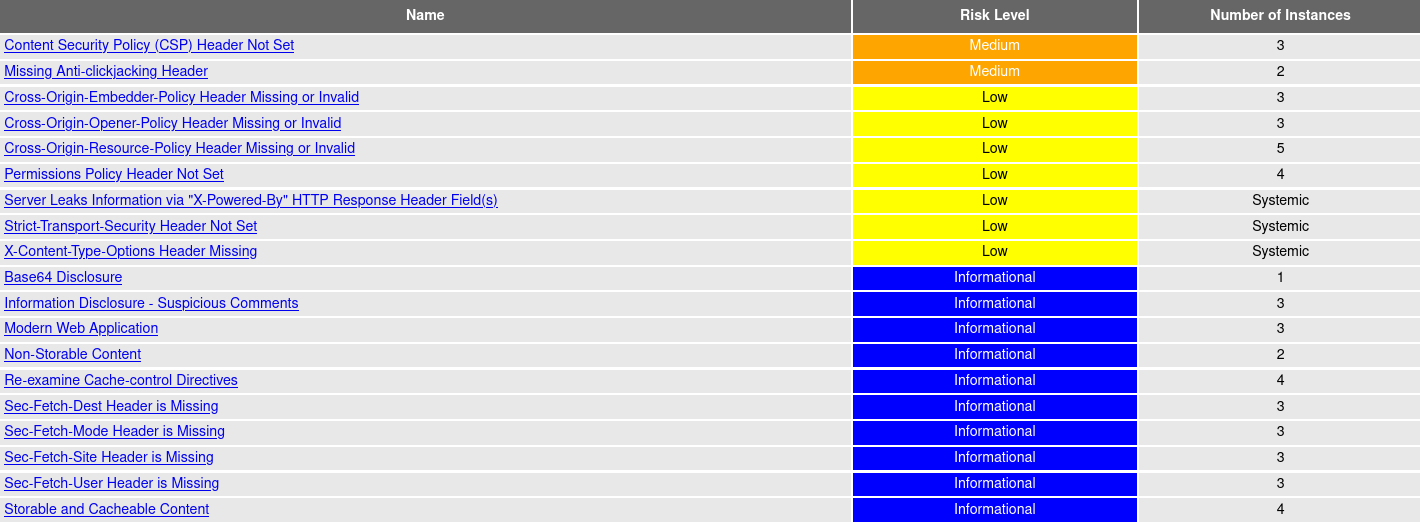
\includegraphics[width=0.95\textwidth,keepaspectratio]{images/screenshots/owasp-zap-alerts-summary}
    \caption{Résumé des alertes OWASP ZAP avant durcissement nginx}
    \label{fig:zap_report}
\end{figure}

\begin{figure}[H]
    \centering
    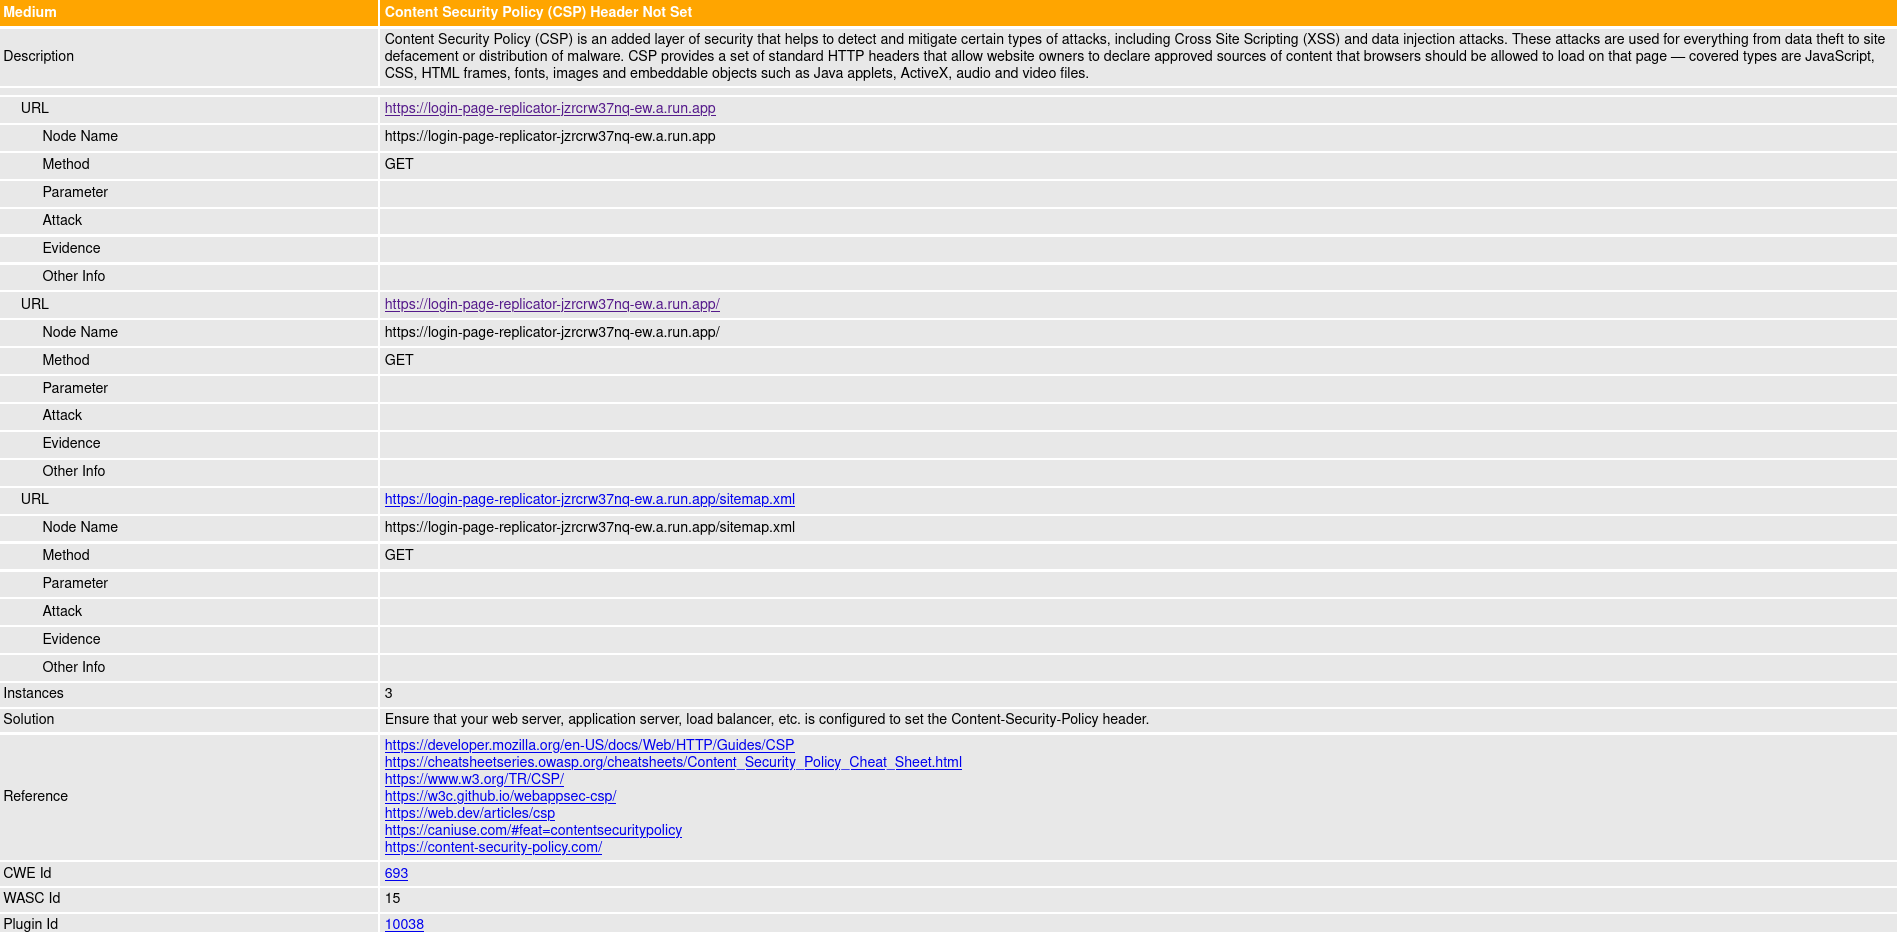
\includegraphics[width=0.95\textwidth,keepaspectratio]{images/screenshots/owasp-zap-csp-header-not-set-details}
    \caption{Détail du finding OWASP ZAP~: Content-Security-Policy header manquant}
    \label{fig:zap_csp_detail}
\end{figure}

\subsection{GitOps avec Argo CD}

\subsubsection{Configuration de l'Application Argo CD}

\begin{lstlisting}[language=bash, caption=Configuration Application Argo CD]
apiVersion: argoproj.io/v1alpha1
kind: Application
metadata:
  name: login-page-replicator
  namespace: argocd
spec:
  source:
    repoURL: https://github.com/nnaffati/login-page-replicator
    targetRevision: HEAD
    path: k8s/app
  destination:
    server: https://kubernetes.default.svc
    namespace: app
  syncPolicy:
    automated:
      prune: true     # Supprime les ressources obsoletes
      selfHeal: true  # Corrige tout drift manuel
    syncOptions:
      - CreateNamespace=true
\end{lstlisting}

\begin{figure}[H]
    \centering
    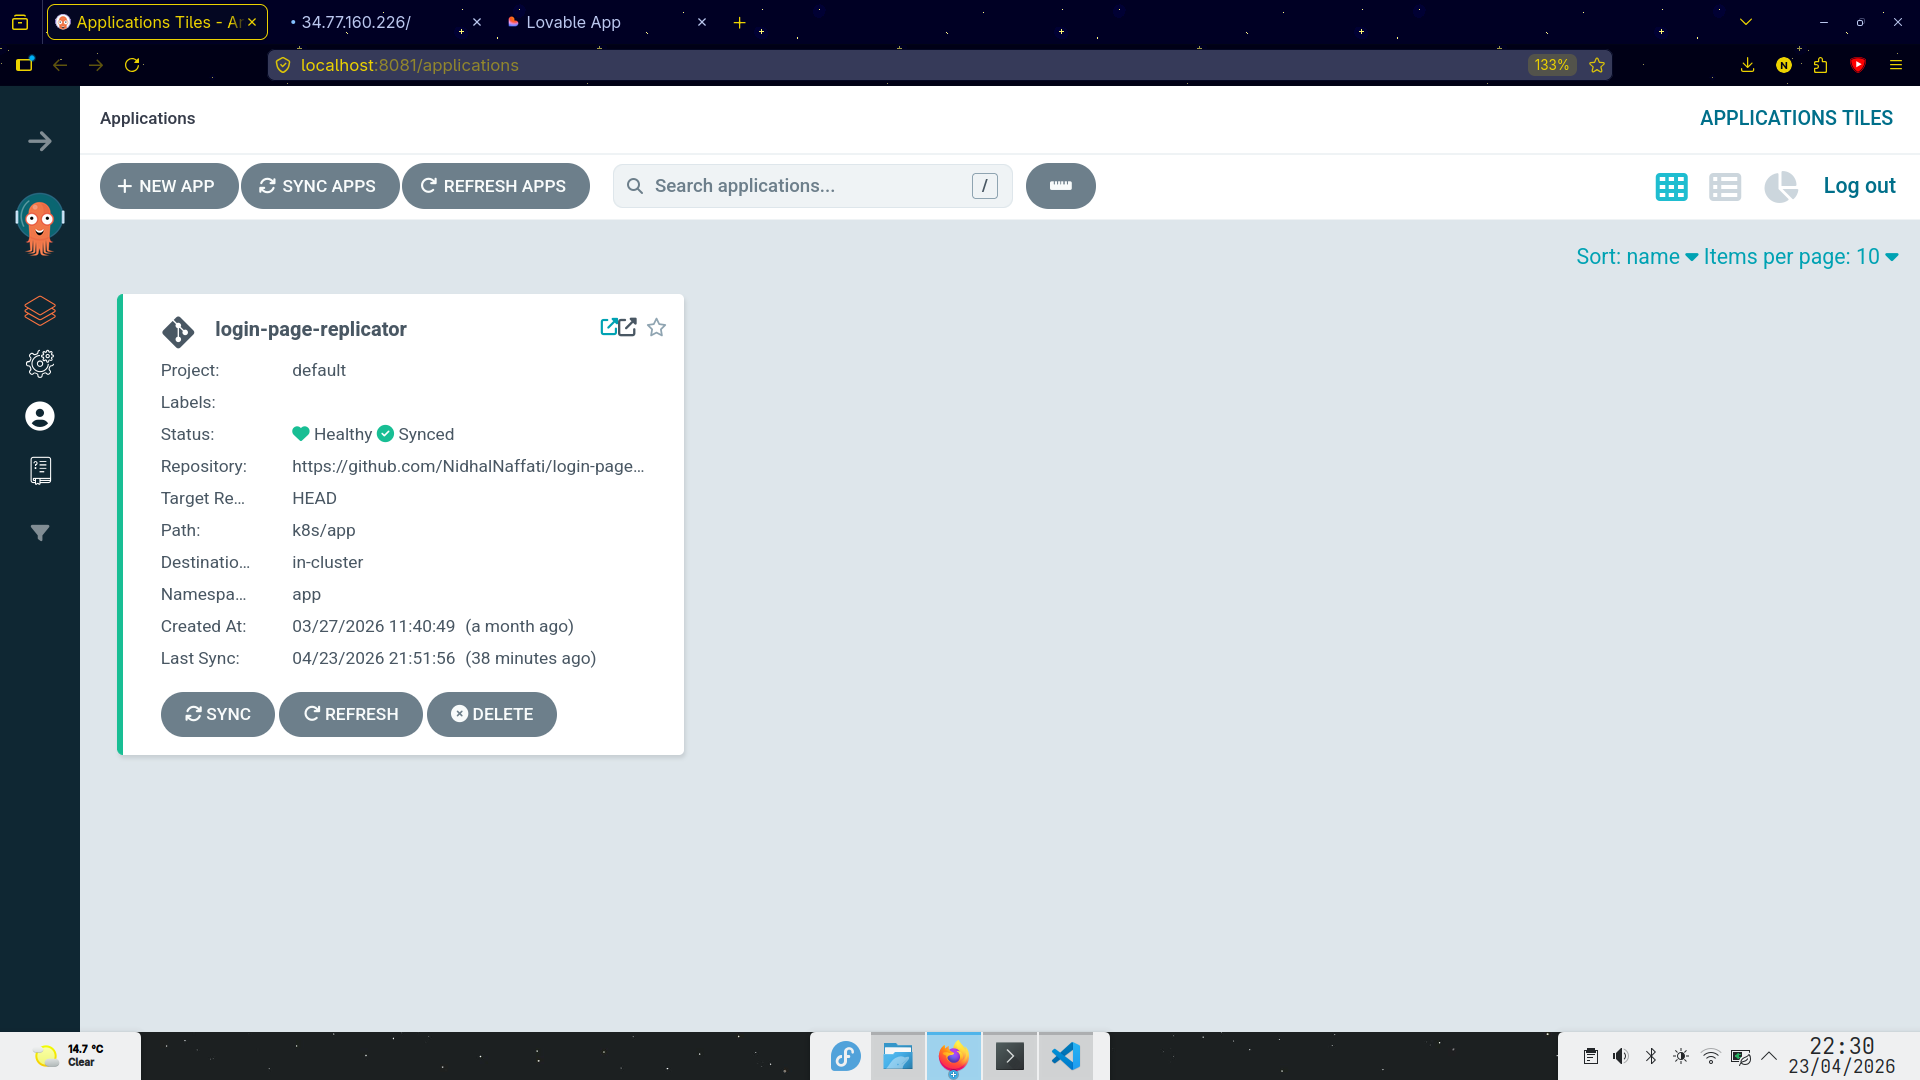
\includegraphics[width=0.95\textwidth,keepaspectratio]{images/screenshots/argocd-applications-tiles-login-page-replicator}
    \caption{Dashboard Argo CD~: vue en tuiles de l'application login-page-replicator}
    \label{fig:argocd_dashboard}
\end{figure}

\begin{figure}[H]
    \centering
    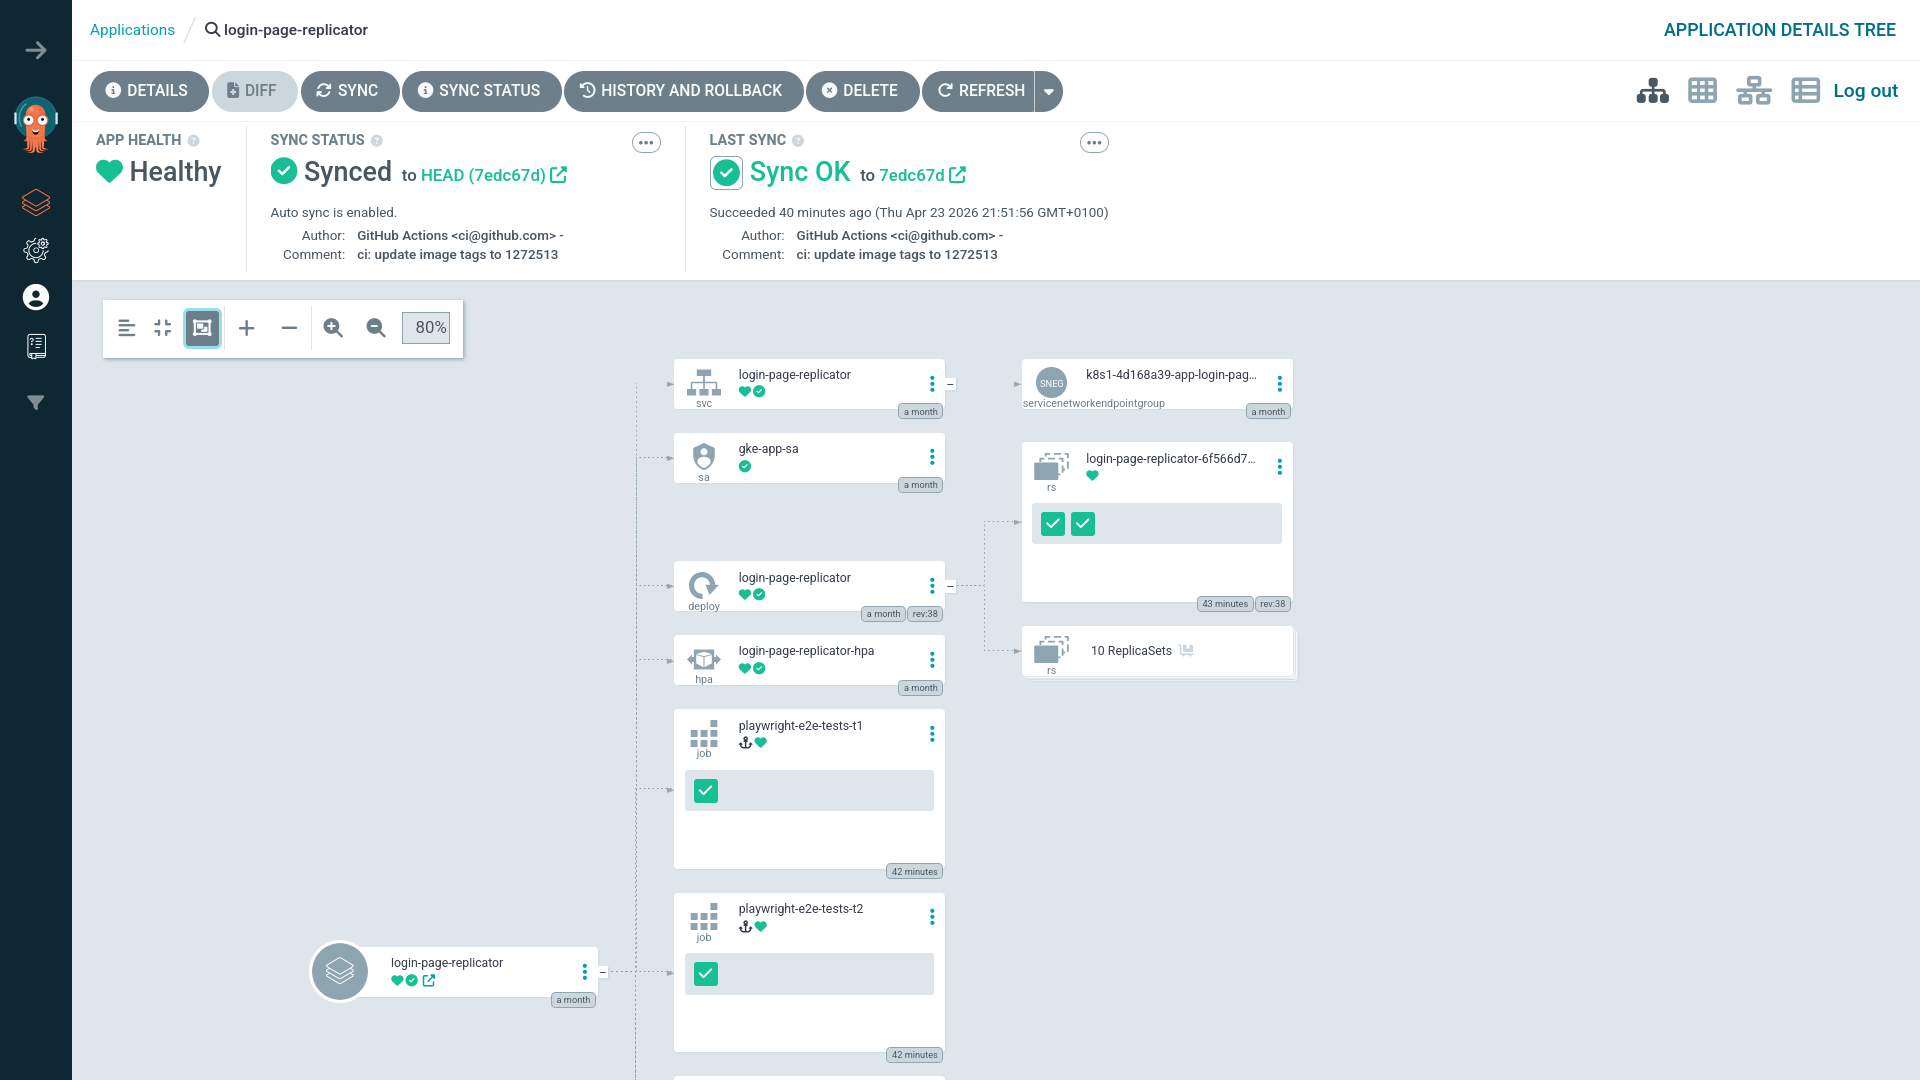
\includegraphics[width=0.95\textwidth,keepaspectratio]{images/screenshots/argocd-application-details-tree-view}
    \caption{Argo CD~: vue arborescente des ressources Kubernetes déployées}
    \label{fig:argocd_tree}
\end{figure}

\begin{figure}[H]
    \centering
    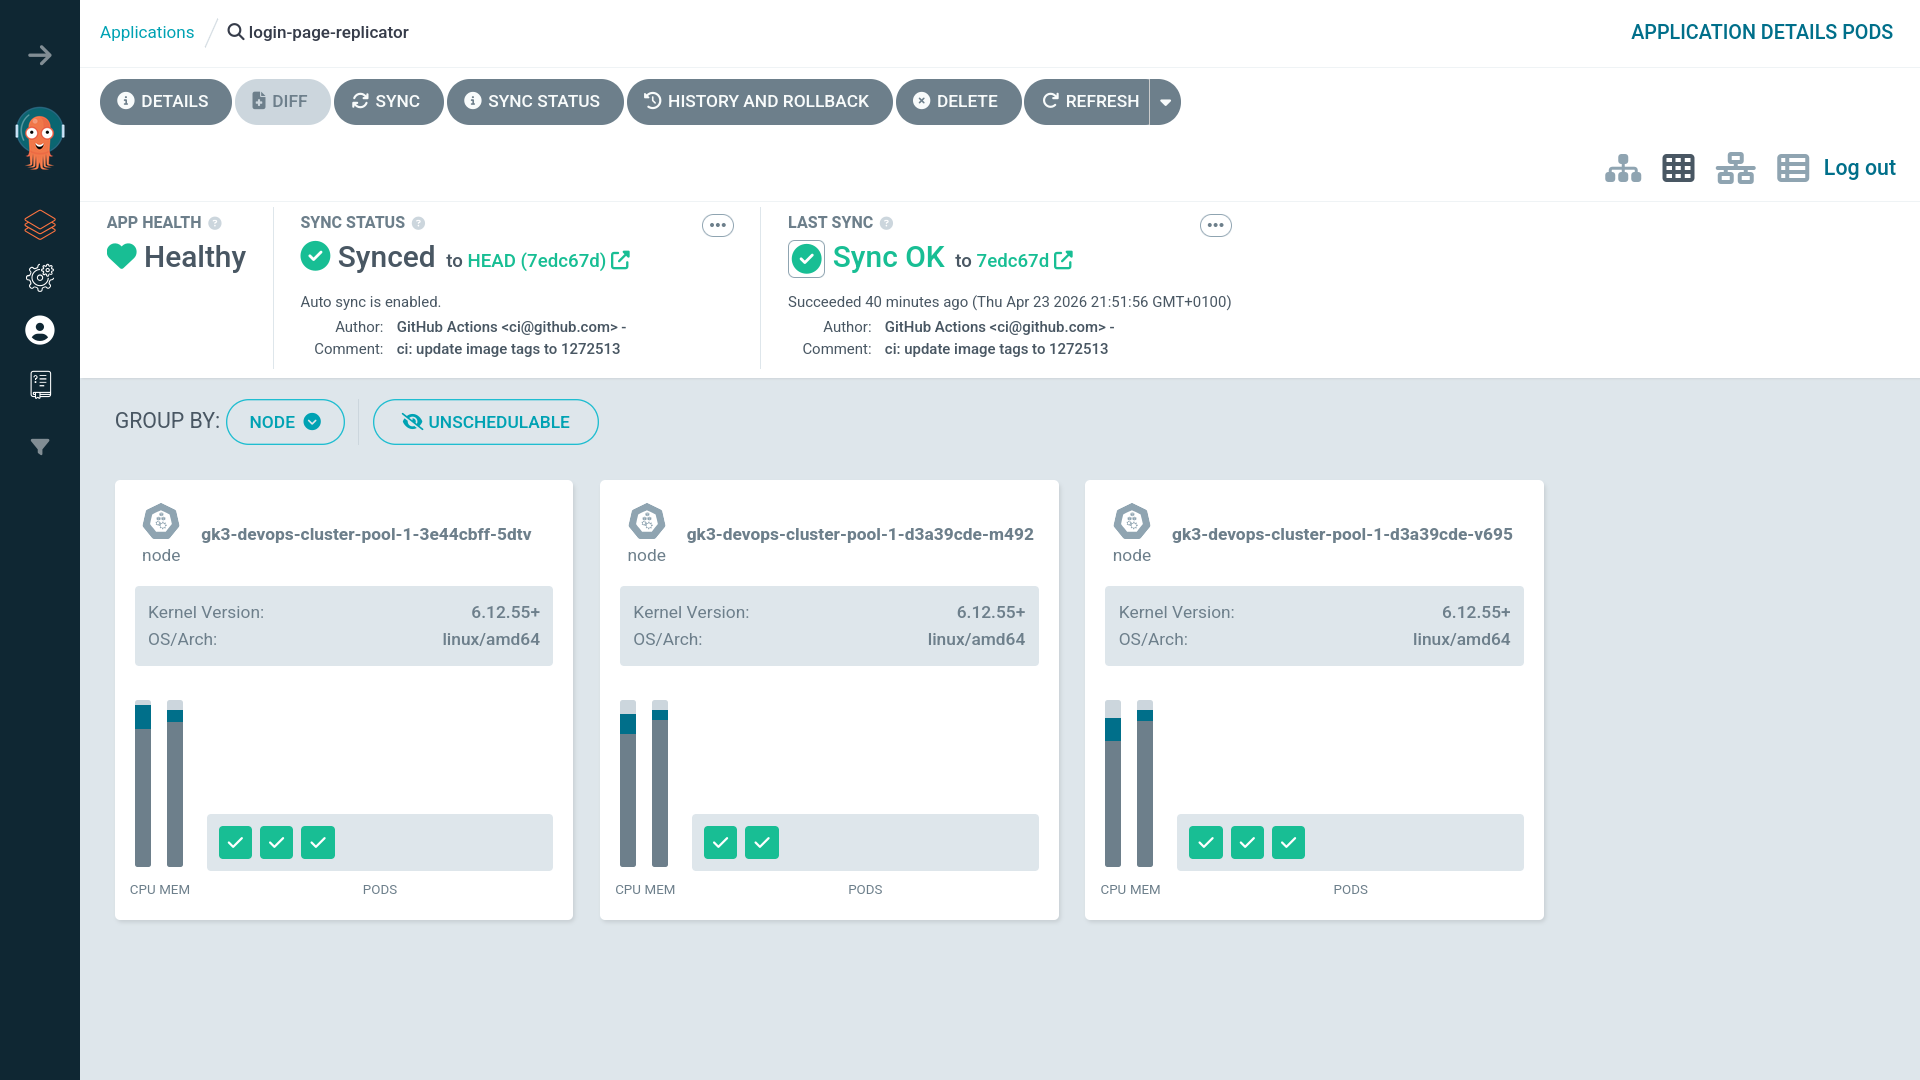
\includegraphics[width=0.95\textwidth,keepaspectratio]{images/screenshots/argocd-application-details-pods-view}
    \caption{Argo CD~: vue des pods de l'application déployée}
    \label{fig:argocd_pods}
\end{figure}

\begin{figure}[H]
    \centering
    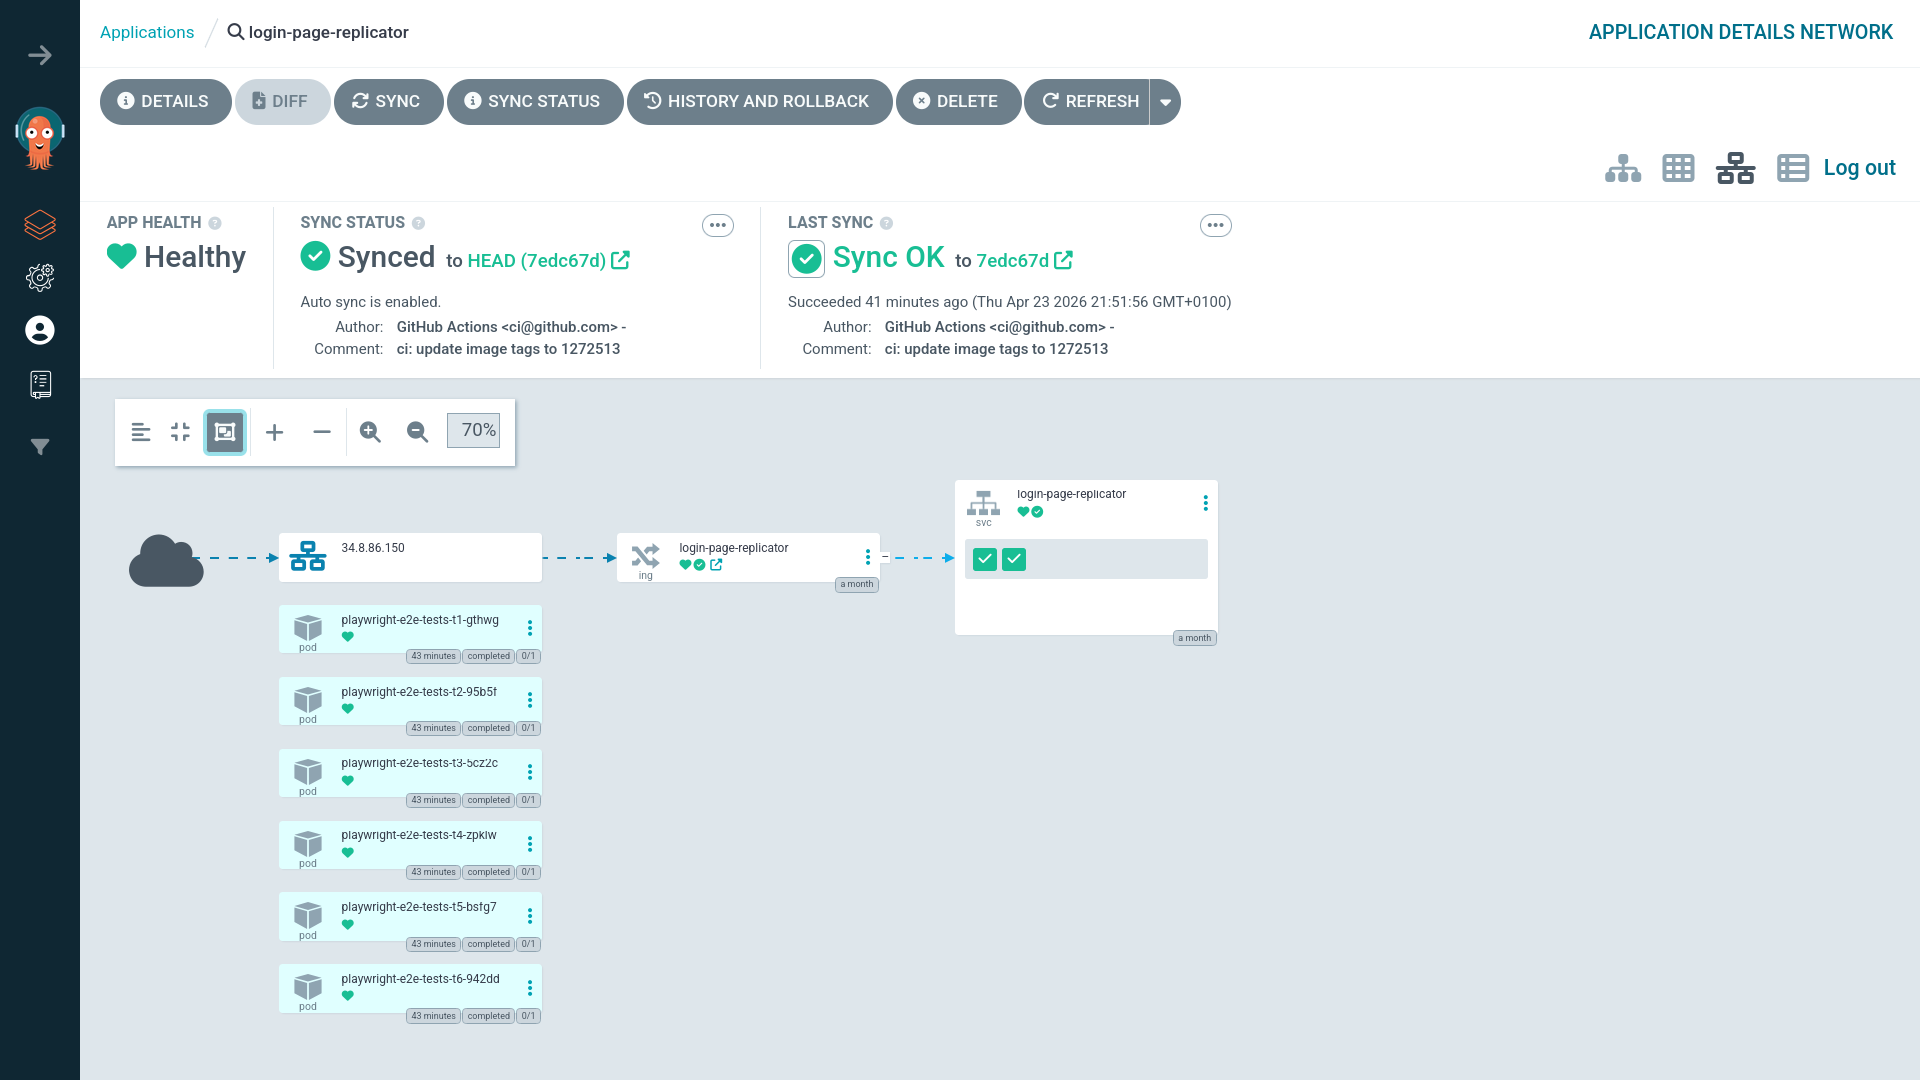
\includegraphics[width=0.95\textwidth,keepaspectratio]{images/screenshots/argocd-application-details-network-view}
    \caption{Argo CD~: vue réseau montrant les flux entre les ressources}
    \label{fig:argocd_network}
\end{figure}

\subsection{Réseau Zero Trust --- NetworkPolicies}

Le projet applique un modèle de \textbf{défense en profondeur} (\textit{Defense in Depth})
superposant plusieurs couches de contrôles indépendantes~:

\begin{table}[H]
\centering
\setlength{\arrayrulewidth}{0.8pt}
\setlength{\dashlinedash}{3pt}
\setlength{\dashlinegap}{2pt}
\renewcommand{\arraystretch}{1.4}
\caption{Modèle de défense en profondeur appliqué au projet}
\label{tab:defense_profondeur}
\begin{tabularx}{\textwidth}{|>{\centering\arraybackslash}X|>{\centering\arraybackslash}X|>{\centering\arraybackslash}X|}
\hline
\tableheader \textbf{Couche} & \textbf{Mécanisme} & \textbf{Portée} \\
\hline
L3/L4~: Périmètre GCP & Pare-feu VPC (Firewall Rules) & Filtrage source/destination entre VM/sous-réseaux \\ \hdashline
L3/L4~: Intra-cluster & NetworkPolicies Kubernetes & Filtrage pod-à-pod, namespace-à-namespace \\ \hdashline
L7~: Admission & Pod Security Standards (GKE Autopilot) & Rejet des manifests non conformes \\ \hdashline
L7~: Application & Headers HTTP durcis (nginx.conf) & Protection navigateur (CSP, HSTS, X-Frame) \\ \hdashline
Identité & Workload Identity Federation + KSA/GSA & Authentification sans clé persistante \\ \hdashline
Détection & Wazuh SIEM + Prometheus alertes & Corrélation logs, détection anomalies \\ \hdashline
Supply Chain & Trivy SCA + Image Scan + Secrets Scan & Analyse avant déploiement \\
\hline
\end{tabularx}
\end{table}

La figure~\ref{fig:defense_profondeur} illustre visuellement l'emboîtement de ces sept couches
de sécurité autour de l'application déployée.

\begin{figure}[H]
    \centering
    \includegraphics[width=0.95\textwidth,keepaspectratio]{images/defense-en-profondeur}
    \caption{Modèle de défense en profondeur --- 7 couches de sécurité}
    \label{fig:defense_profondeur}
\end{figure}

\subsubsection{Principe Default-Deny}

Sans NetworkPolicies, tous les pods communiquent librement. La politique appliquée~:
\textbf{tout est interdit par défaut, chaque flux autorisé est déclaré explicitement}.
Une politique \texttt{default-deny-all} est appliquée dans les quatre namespaces
(\texttt{app}, \texttt{testing}, \texttt{observability}, \texttt{security})~:

\begin{lstlisting}[language=bash, caption=Politique default-deny appliquée à chaque namespace]
apiVersion: networking.k8s.io/v1
kind: NetworkPolicy
metadata:
  name: default-deny-all
  namespace: app    # Replique pour: testing, observability, security
spec:
  podSelector: {}   # Selectionne TOUS les pods du namespace
  policyTypes:
    - Ingress       # Bloque tout trafic entrant
    - Egress        # Bloque tout trafic sortant
\end{lstlisting}

Sans exception explicite, aucun pod ne peut communiquer avec un autre, ni résoudre un nom
DNS, ni recevoir de health check. Chaque flux légitime est déclaré via une NetworkPolicy dédiée.

\subsubsection{Inventaire Complet des NetworkPolicies}

Le projet déploie \textbf{12 NetworkPolicies} organisées par responsabilité~:

\begin{table}[H]
\centering
\setlength{\arrayrulewidth}{0.8pt}
\setlength{\dashlinedash}{3pt}
\setlength{\dashlinegap}{2pt}
\renewcommand{\arraystretch}{1.4}
\caption{Inventaire complet des 12 NetworkPolicies déployées}
\label{tab:netpol_inventory}
\begin{tabularx}{\textwidth}{|>{\centering\arraybackslash}X|>{\centering\arraybackslash}X|>{\centering\arraybackslash}X|}
\hline
\tableheader \textbf{Politique} & \textbf{Namespace(s)} & \textbf{Rôle} \\
\hline
default-deny-all & app, testing, observability, security & Bloque tout ingress + egress \\ \hdashline
allow-dns-egress & app, testing, observability, security & Autorise UDP/TCP 53 (CoreDNS) \\ \hdashline
allow-kubelet-probes-app & app & Probes depuis nœuds + GCP LB \\ \hdashline
allow-kubelet-probes & observability & Probes sur ports 3000, 8080, 8081, 9090 \\ \hdashline
allow-prometheus-scrape & app (ingress) & Scrape depuis ns observability sur 9113 \\ \hdashline
allow-observability-to-app-metrics & observability (egress) & Egress vers app:9113 \\ \hdashline
allow-observability-internal & observability & Pod-à-pod interne \\ \hdashline
allow-apiserver-egress & observability & Egress HTTPS/443 vers API server K8s \\ \hdashline
allow-testing-to-app-http & testing + app & Tests E2E vers app sur TCP 80 \\ \hdashline
allow-playwright-hook-egress & app (egress hook) & Hook PostSync vers app:80 \\ \hdashline
allow-playwright-hook-to-app & app (ingress) & App accepte trafic du hook \\ \hdashline
allow-wazuh-agent-egress & security & Agent $\to$ Manager 10.10.0.2 sur TCP 1514/1515 \\
\hline
\end{tabularx}
\end{table}

\subsubsection{Matrice des Flux Autorisés}

\begin{table}[H]
\centering
\setlength{\arrayrulewidth}{0.8pt}
\setlength{\dashlinedash}{3pt}
\setlength{\dashlinegap}{2pt}
\renewcommand{\arraystretch}{1.4}
\caption{Matrice des flux réseau autorisés}
\label{tab:network_matrix}
\begin{tabularx}{\textwidth}{|>{\centering\arraybackslash}X|>{\centering\arraybackslash}X|>{\centering\arraybackslash}X|>{\centering\arraybackslash}X|}
\hline
\tableheader \textbf{Source} & \textbf{Destination} & \textbf{Port} & \textbf{Politique} \\
\hline
\texttt{testing} pods & \texttt{app} pods & TCP 80 & allow-testing-to-app \\ \hdashline
PostSync hook & \texttt{app} pods & TCP 80 & allow-playwright-hook \\ \hdashline
\texttt{observability} & \texttt{app} sidecar & TCP 9113 & allow-prometheus-scrape \\ \hdashline
\texttt{observability} pods & \texttt{observability} pods & Tous & allow-observability-internal \\ \hdashline
\texttt{observability} pods & API Server K8s & TCP 443 & allow-apiserver-egress \\ \hdashline
\texttt{security} DaemonSet & Wazuh VM (10.10.0.2) & TCP 1514/1515 & allow-wazuh-egress \\ \hdashline
Tous les pods & kube-dns (CoreDNS) & UDP/TCP 53 & allow-dns-egress \\ \hdashline
Nœuds (10.10.0.0/20) & \texttt{app} pods & TCP 80, 9113 & allow-kubelet-probes-app \\ \hdashline
GCP LB (130.211.0.0/22, 35.191.0.0/16) & \texttt{app} pods & TCP 80, 9113 & allow-kubelet-probes-app \\
\hline
\end{tabularx}
\end{table}

La figure~\ref{fig:network_zero_trust} fournit une vue d'ensemble des flux autorisés entre les
différents namespaces, le DNS, les nœuds (kubelet) et la VM Wazuh.

\begin{figure}[H]
    \centering
    \includegraphics[width=0.95\textwidth,keepaspectratio]{images/network-zero-trust}
    \caption{Topologie Zero Trust --- flux autorisés entre namespaces et composants externes}
    \label{fig:network_zero_trust}
\end{figure}

\subsubsection{Exemples de Politiques Cross-Namespace}

\begin{lstlisting}[language=bash, caption=allow-prometheus-scrape~: cross-namespace ingress]
apiVersion: networking.k8s.io/v1
kind: NetworkPolicy
metadata:
  name: allow-prometheus-scrape
  namespace: app
spec:
  podSelector: {}
  policyTypes:
    - Ingress
  ingress:
    - from:
        - namespaceSelector:
            matchLabels:
              kubernetes.io/metadata.name: observability
      ports:
        - port: 9113    # Seulement le port du sidecar nginx-exporter
\end{lstlisting}

\begin{lstlisting}[language=bash, caption=allow-wazuh-agent-egress~: filtrage par IP exacte]
apiVersion: networking.k8s.io/v1
kind: NetworkPolicy
metadata:
  name: allow-wazuh-agent-egress
  namespace: security
spec:
  podSelector:
    matchLabels:
      app: wazuh-agent
  policyTypes:
    - Egress
  egress:
    - to:
        - ipBlock:
            cidr: 10.10.0.2/32    # IP exacte du Wazuh Manager
      ports:
        - protocol: TCP
          port: 1514              # Communication agent
        - protocol: TCP
          port: 1515              # Enregistrement agent
\end{lstlisting}

\subsection{Pare-feu GCP --- Règles de Filtrage VPC}

En complément des NetworkPolicies (niveau pod), des règles de pare-feu GCP sont appliquées
au niveau VPC pour contrôler le trafic entre les VM, les sous-réseaux et Internet~:

\begin{table}[H]
\centering
\setlength{\arrayrulewidth}{0.8pt}
\setlength{\dashlinedash}{3pt}
\setlength{\dashlinegap}{2pt}
\renewcommand{\arraystretch}{1.4}
\caption{Plan d'adressage IP du VPC \texttt{devops-vpc}}
\label{tab:ip_plan}
\begin{tabularx}{\textwidth}{|>{\centering\arraybackslash}X|>{\centering\arraybackslash}X|>{\centering\arraybackslash}X|}
\hline
\tableheader \textbf{Plage} & \textbf{CIDR} & \textbf{Usage} \\
\hline
Subnet principal (nœuds) & 10.10.0.0/20 & Nœuds GKE + VM Wazuh \\ \hdashline
Plage secondaire pods & 10.20.0.0/16 & Adresses IP pods (65~536 adresses) \\ \hdashline
Plage secondaire services & 10.30.0.0/20 & ClusterIPs des services K8s \\
\hline
\end{tabularx}
\end{table}

\begin{table}[H]
\centering
\setlength{\arrayrulewidth}{0.8pt}
\setlength{\dashlinedash}{3pt}
\setlength{\dashlinegap}{2pt}
\renewcommand{\arraystretch}{1.4}
\caption{Règles de pare-feu GCP pour Wazuh SIEM}
\label{tab:firewall_rules}
\begin{tabularx}{\textwidth}{|>{\centering\arraybackslash}X|>{\centering\arraybackslash}X|>{\centering\arraybackslash}X|>{\centering\arraybackslash}X|}
\hline
\tableheader \textbf{Règle} & \textbf{Ports} & \textbf{Source} & \textbf{Justification} \\
\hline
allow-wazuh-agents & TCP 1514, 1515, 55000 & 10.10.0.0/20 + 10.20.0.0/16 & Agents $\to$ manager \\ \hdashline
allow-wazuh-dashboard & TCP 443 & 0.0.0.0/0 (restreindre en prod) & Dashboard Wazuh \\ \hdashline
allow-ssh-wazuh & TCP 22 & 35.235.240.0/20 (IAP only) & SSH via IAP tunnel \\
\hline
\end{tabularx}
\end{table}

\textbf{Points de sécurité notables~:}
\begin{itemize}
  \item L'accès SSH est restreint aux plages IP de \textbf{Identity-Aware Proxy (IAP)}
        (\texttt{35.235.240.0/20}), empêchant tout accès SSH direct depuis Internet~;
  \item Les agents ne communiquent qu'avec le manager depuis les plages internes du VPC~;
  \item Le \textbf{target tag} \texttt{wazuh-manager} isole les règles à la seule VM concernée.
\end{itemize}

\begin{lstlisting}[language=bash, caption=Règle pare-feu Terraform~: SSH via IAP uniquement]
resource "google_compute_firewall" "wazuh_ssh" {
  name    = "allow-ssh-wazuh"
  network = google_compute_network.vpc.name
  allow {
    protocol = "tcp"
    ports    = ["22"]
  }
  # IAP range - gcloud compute ssh sans exposer le port 22
  source_ranges = ["35.235.240.0/20"]
  target_tags   = ["wazuh-manager"]
}
\end{lstlisting}

La figure~\ref{fig:archi_reseau_gcp} présente l'architecture réseau complète du VPC,
avec le positionnement du cluster GKE, de la VM Wazuh et des règles de pare-feu associées.

\begin{figure}[H]
    \centering
    \includegraphics[width=0.95\textwidth,keepaspectratio]{images/architecture-reseau-gcp-firewall}
    \caption{Architecture réseau GCP --- VPC, sous-réseaux, pare-feu et Wazuh}
    \label{fig:archi_reseau_gcp}
\end{figure}

\subsection{Pod Security Standards --- GKE Autopilot}

GKE Autopilot impose les \textbf{Pod Security Standards} (PSS) au niveau \texttt{restricted}.
Tout manifest non conforme est \textbf{rejeté à l'admission}~:

\begin{table}[H]
\centering
\setlength{\arrayrulewidth}{0.8pt}
\setlength{\dashlinedash}{3pt}
\setlength{\dashlinegap}{2pt}
\renewcommand{\arraystretch}{1.4}
\caption{Contrôles Pod Security Standards imposés par GKE Autopilot}
\label{tab:pss}
\begin{tabularx}{\textwidth}{|>{\centering\arraybackslash}X|>{\centering\arraybackslash}X|>{\centering\arraybackslash}X|}
\hline
\tableheader \textbf{Contrôle} & \textbf{Comportement rejeté} & \textbf{Impact sécurité} \\
\hline
\texttt{privileged: true} & Accès root au nœud & Empêche l'évasion de conteneur \\ \hdashline
\texttt{hostNetwork: true} & Accès réseau du nœud & Empêche le sniffing réseau \\ \hdashline
\texttt{hostPID: true} & Vision des processus hôte & Empêche l'espionnage inter-conteneur \\ \hdashline
\texttt{capabilities: SYS\_ADMIN} & Capacité admin complète & Réduit la surface d'attaque \\ \hdashline
Volumes \texttt{hostPath} sensibles & Montage de répertoires critiques & Protège le filesystem hôte \\
\hline
\end{tabularx}
\end{table}

Le fichier \texttt{k8s/vulnerable-demo/deployment.yaml} contient intentionnellement toutes
les misconfigurations (pour le scan Trivy IaC). Si appliqué, Autopilot le rejetterait~:

\begin{lstlisting}[language=bash, caption=Manifest vulnérable (rejeté par Autopilot)]
securityContext:
  privileged: true      # REJETE par Autopilot
  runAsUser: 0          # REJETE par Autopilot
  capabilities:
    add: [NET_ADMIN, SYS_ADMIN, ALL]  # REJETE
hostNetwork: true       # REJETE par Autopilot
hostPID: true           # REJETE par Autopilot
\end{lstlisting}

\subsection{Rétrospective Sprint 3}

\begin{table}[H]
\centering
\setlength{\arrayrulewidth}{0.8pt}
\renewcommand{\arraystretch}{1.4}
\caption{Rétrospective Sprint 3}
\label{tab:retro_s3}
\begin{tabularx}{\textwidth}{|>{\centering\arraybackslash}X|X|}
\hline
\tableheader \textbf{Catégorie} & \textbf{Détail} \\
\hline
Ce qui a bien marché & Tous les scans de sécurité détectent les vulnérabilités attendues, Argo CD auto-sync opérationnel \\
\hline
Difficultés & Gestion des faux positifs Trivy/ZAP, orchestration des NetworkPolicies avec les PostSync hooks \\
\hline
Livrable & Sécurité SAST/SCA/DAST intégrée, GitOps opérationnel, réseau Zero Trust \\
\hline
\end{tabularx}
\end{table}


%% ================================================================
%%  SPRINT 4 — Tests E2E, Observabilité, SIEM et Bilan
%% ================================================================
\section{Sprint 4~: Tests E2E, Observabilité, SIEM et Bilan}

\subsection{Objectif et Backlog du Sprint}

\begin{table}[H]
\centering
\setlength{\arrayrulewidth}{0.8pt}
\setlength{\dashlinedash}{3pt}
\setlength{\dashlinegap}{2pt}
\renewcommand{\arraystretch}{1.4}
\caption{Backlog du Sprint 4}
\label{tab:backlog_s4}
\begin{tabularx}{\textwidth}{|>{\centering\arraybackslash}X|>{\centering\arraybackslash}X|>{\centering\arraybackslash}X|}
\hline
\tableheader \textbf{User Story} & \textbf{Tâche} & \textbf{Statut} \\
\hline
US-10~: Playwright E2E & Écrire 6 scénarios Playwright (@t1 à @t6) & Terminé \\ \hdashline
US-10 & Configurer l'exécution in-cluster (PostSync + standalone Job) & Terminé \\ \hdashline
US-11~: Observabilité & Déployer Prometheus + Grafana dans le namespace observability & Terminé \\ \hdashline
US-11 & Configurer le ServiceMonitor pour le sidecar nginx-exporter & Terminé \\ \hdashline
US-12~: Wazuh SIEM & Déployer le DaemonSet Wazuh Agent dans le namespace security & Terminé \\ \hdashline
US-12 & Connecter les agents au manager Wazuh sur la VM & Terminé \\
\hline
\end{tabularx}
\end{table}

\subsection{Tests Unitaires avec Vitest}

Les tests unitaires couvrent les composants React critiques~:
\begin{itemize}
  \item \textbf{TodoItem}~: rendu du texte, toggle completed, suppression~;
  \item \textbf{AuthContext}~: login/logout, persistence de session~;
  \item \textbf{TodoDashboard}~: CRUD complet, filtrage, compteurs.
\end{itemize}

La couverture de code mesurée par Vitest est de \textbf{13\%} sur l'ensemble du projet.
Cette couverture est volontairement limitée car la priorité du projet porte sur
l'infrastructure DevSecOps et les pipelines de sécurité plutôt que sur la couverture
unitaire exhaustive d'une application de démonstration.

%% TODO: Update this figure with actual vitest coverage screenshot
\begin{figure}[H]
    \centering
    \fbox{\parbox{0.85\textwidth}{\centering
        \vspace{2.5cm}
        Espace réservé pour la Figure~\ref{fig:vitest_coverage}\\
        \textbf{Capture d'écran~: Rapport de couverture Vitest}
        \vspace{2.5cm}
    }}
    \caption{Rapport de couverture des tests unitaires Vitest}
    \label{fig:vitest_coverage}
\end{figure}

\subsection{Tests E2E Playwright --- 6 Scénarios}

\begin{table}[H]
\centering
\setlength{\arrayrulewidth}{0.8pt}
\setlength{\dashlinedash}{3pt}
\setlength{\dashlinegap}{2pt}
\renewcommand{\arraystretch}{1.4}
\caption{Les 6 scénarios de tests Playwright E2E}
\label{tab:playwright}
\begin{tabularx}{\textwidth}{|>{\centering\arraybackslash}X|>{\centering\arraybackslash}X|>{\centering\arraybackslash}X|}
\hline
\tableheader \textbf{Tag} & \textbf{Scénario} & \textbf{Ce que ça valide} \\
\hline
@t1 & Credentials invalides $\to$ message d'erreur & Authentification, gestion erreurs \\ \hdashline
@t2 & Login $\to$ dashboard vide affiché & Flux d'authentification complet \\ \hdashline
@t3 & Login $\to$ Logout $\to$ retour formulaire & Cycle auth complet \\ \hdashline
@t4 & Session persiste après rechargement & Persistance localStorage \\ \hdashline
@t5 & Todos persistent après rechargement & Persistance des données \\ \hdashline
@t6 & Ajouter, compléter, supprimer une tâche & CRUD complet \\
\hline
\end{tabularx}
\end{table}

Les tests sont exécutés en trois modes~:
\begin{itemize}
  \item \textbf{In-cluster (PostSync)}~: jobs Kubernetes créés par Argo CD après chaque
        déploiement~;
  \item \textbf{Local CI (matrice)}~: GitHub Actions exécute Playwright avec \texttt{--grep
        @t1..@t6}~;
  \item \textbf{Standalone Job}~: \texttt{k8s/testing/playwright-job.yaml} pour tests manuels.
\end{itemize}

\begin{figure}[H]
    \centering
    \fbox{\parbox{0.85\textwidth}{\centering
        \vspace{2.5cm}
        Espace réservé pour la Figure~\ref{fig:playwright_results}\\
        \textbf{Capture d'écran~: Résultats des 6 tests Playwright E2E}
        \vspace{2.5cm}
    }}
    \caption{Résultats des tests Playwright E2E (6/6 passed)}
    \label{fig:playwright_results}
\end{figure}

\subsection{Observabilité avec Prometheus et Grafana}

Le flux de collecte des métriques~:
\begin{enumerate}
  \item Le sidecar \texttt{nginx-exporter} (port 9113) expose les métriques Nginx~;
  \item Le \texttt{ServiceMonitor} scrape ces métriques toutes les 30 secondes~;
  \item Prometheus stocke les séries temporelles~;
  \item Grafana interroge Prometheus pour les tableaux de bord.
\end{enumerate}

\begin{table}[H]
\centering
\setlength{\arrayrulewidth}{0.8pt}
\setlength{\dashlinedash}{3pt}
\setlength{\dashlinegap}{2pt}
\renewcommand{\arraystretch}{1.4}
\caption{Métriques Nginx collectées et leur utilité sécurité}
\label{tab:metrics}
\begin{tabularx}{\textwidth}{|>{\centering\arraybackslash}X|>{\centering\arraybackslash}X|>{\centering\arraybackslash}X|}
\hline
\tableheader \textbf{Métrique} & \textbf{Description} & \textbf{Utilité Sécurité} \\
\hline
nginx\_connections\_active & Connexions actives & Détection de DDoS \\ \hdashline
nginx\_http\_requests\_total & Requêtes par status code & Spike de 4xx = attaque de scan \\ \hdashline
nginx\_connections\_accepted & Connexions acceptées total & Baseline trafic normal \\ \hdashline
nginx\_connections\_handled & Connexions traitées & Performance et disponibilité \\
\hline
\end{tabularx}
\end{table}

\begin{figure}[H]
    \centering
    \fbox{\parbox{0.85\textwidth}{\centering
        \vspace{2.5cm}
        Espace réservé pour la Figure~\ref{fig:grafana_dashboard}\\
        \textbf{Capture d'écran~: Dashboard Grafana avec métriques Nginx}
        \vspace{2.5cm}
    }}
    \caption{Dashboard Grafana montrant les métriques Nginx en temps réel}
    \label{fig:grafana_dashboard}
\end{figure}

\subsection{Sécurité Runtime --- Wazuh SIEM}

Wazuh est un SIEM open-source qui fournit~: détection d'intrusion (HIDS), monitoring de
l'intégrité des fichiers (FIM), conformité réglementaire (PCI DSS, GDPR, NIST), et
corrélation d'événements en temps réel.

L'architecture Wazuh se compose de~:
\begin{itemize}
  \item \textbf{Wazuh Manager}~: VM GCE \texttt{e2-medium} (Ubuntu 22.04, 50~Go) hébergeant
        Manager + Indexer + Dashboard, provisionnée par Terraform~;
  \item \textbf{Wazuh Agents}~: DaemonSet dans le namespace \texttt{security},
        une instance par nœud.
\end{itemize}

\subsubsection{Configuration du DaemonSet Agent}

\begin{lstlisting}[language=bash, caption=Configuration Wazuh Agent (ossec.conf)]
<ossec_config>
  <client>
    <server>
      <address>10.10.0.2</address>
      <port>1514</port>
      <protocol>tcp</protocol>
    </server>
    <auto_restart>yes</auto_restart>
  </client>
  <wodle name="syscollector">
    <disabled>no</disabled>
    <interval>1h</interval>
    <os>yes</os>
    <network>yes</network>
    <ports>yes</ports>
  </wodle>
  <localfile>
    <log_format>syslog</log_format>
    <location>/var/log/containers/*.log</location>
  </localfile>
  <localfile>
    <log_format>syslog</log_format>
    <location>/var/log/pods/*/*/*.log</location>
  </localfile>
</ossec_config>
\end{lstlisting}

\begin{lstlisting}[language=bash, caption=DaemonSet Wazuh Agent avec contraintes de ressources]
apiVersion: apps/v1
kind: DaemonSet
metadata:
  name: wazuh-agent
  namespace: security
spec:
  selector:
    matchLabels:
      app: wazuh-agent
  template:
    spec:
      containers:
        - name: wazuh-agent
          image: wazuh/wazuh-agent:4.14.4
          volumeMounts:
            - name: varlog
              mountPath: /var/log
              readOnly: true
          resources:
            requests: { cpu: "100m", memory: "128Mi" }
            limits:   { cpu: "200m", memory: "256Mi" }
      volumes:
        - name: varlog
          hostPath:
            path: /var/log
      tolerations:
        - operator: Exists
\end{lstlisting}

\subsubsection{Capacités de Détection sur GKE Autopilot}

\begin{table}[H]
\centering
\setlength{\arrayrulewidth}{0.8pt}
\setlength{\dashlinedash}{3pt}
\setlength{\dashlinegap}{2pt}
\renewcommand{\arraystretch}{1.4}
\caption{Capacités de détection Wazuh sur GKE Autopilot}
\label{tab:wazuh_capabilities}
\begin{tabularx}{\textwidth}{|>{\centering\arraybackslash}X|>{\centering\arraybackslash}X|>{\centering\arraybackslash}X|}
\hline
\tableheader \textbf{Capacité} & \textbf{Statut} & \textbf{Description} \\
\hline
Collecte logs conteneurs & Opérationnel & \texttt{/var/log/containers/*.log} + \texttt{/var/log/pods/} \\ \hdashline
Inventaire réseau & Opérationnel & Ports ouverts, interfaces réseau \\ \hdashline
Détection OS & Opérationnel & Identification OS des nœuds \\ \hdashline
Conformité réglementaire & Opérationnel & Mappings PCI DSS, GDPR, NIST 800-53 \\ \hdashline
Corrélation événements & Opérationnel & Règles de détection sur patterns de logs \\ \hdashline
Audit syscall & Bloqué (Autopilot) & \texttt{hostPID} requis \\ \hdashline
Monitoring processus & Bloqué (Autopilot) & \texttt{/proc} non accessible \\ \hdashline
FIM kernel-level & Bloqué (Autopilot) & Conteneur privilégié requis \\
\hline
\end{tabularx}
\end{table}

\begin{warningbox}
\textbf{Compromis accepté~:} la sécurité renforcée d'Autopilot (empêchant les évasions de
conteneurs) est jugée plus importante que la visibilité kernel complète de Wazuh. En
production, un cluster Standard avec nœuds dédiés offrirait une couverture complète.
\end{warningbox}

\begin{figure}[H]
    \centering
    \fbox{\parbox{0.85\textwidth}{\centering
        \vspace{2.5cm}
        Espace réservé pour la Figure~\ref{fig:wazuh_dashboard}\\
        \textbf{Capture d'écran~: Dashboard Wazuh montrant les agents connectés}
        \vspace{2.5cm}
    }}
    \caption{Dashboard Wazuh avec 4 agents opérationnels}
    \label{fig:wazuh_dashboard}
\end{figure}

\subsection{Gouvernance IAM et Identité}

\subsubsection{Problème des Clés JSON Statiques}

Les clés JSON GCP posent quatre risques majeurs~:
\begin{itemize}
  \item \textbf{Pas d'expiration}~: une clé compromise reste valide indéfiniment~;
  \item \textbf{Rotation manuelle}~: source d'erreur humaine et d'oubli~;
  \item \textbf{Stockage dans CI}~: les secrets GitHub Actions peuvent être exfiltrés~;
  \item \textbf{Blast radius}~: une clé donne accès à tous les rôles IAM associés.
\end{itemize}

\subsubsection{Sécurisation par Attribute Condition (WIF)}

Le provider WIF est configuré avec une condition d'attribut restreignant l'échange de
token au seul repository autorisé~:

\begin{lstlisting}[language=bash, caption=Condition d'attribut WIF sécurisant le pipeline]
resource "google_iam_workload_identity_pool_provider" "github" {
  oidc {
    issuer_uri = "https://token.actions.githubusercontent.com"
  }
  attribute_condition = "attribute.repository == 'NidhalNaffati/login-page-replicator'"
}
\end{lstlisting}

Un fork malveillant ou tout autre repository GitHub sera refusé par le pool WIF.

\subsubsection{Workload Identity --- Pods Kubernetes}

En complément du WIF pour le CI/CD, les pods utilisent \textbf{Workload Identity} pour
s'authentifier auprès des APIs GCP sans clé~:

\begin{table}[H]
\centering
\setlength{\arrayrulewidth}{0.8pt}
\setlength{\dashlinedash}{3pt}
\setlength{\dashlinegap}{2pt}
\renewcommand{\arraystretch}{1.4}
\caption{Bindings Workload Identity (KSA $\to$ GSA)}
\label{tab:workload_identity}
\begin{tabularx}{\textwidth}{|>{\centering\arraybackslash}X|>{\centering\arraybackslash}X|>{\centering\arraybackslash}X|}
\hline
\tableheader \textbf{KSA (Kubernetes)} & \textbf{GSA (GCP)} & \textbf{Namespace} \\
\hline
gke-app-sa & gke-app-sa@pfe-esprit-489411.iam & app \\ \hdashline
playwright-runner & gke-app-sa@pfe-esprit-489411.iam & testing \\ \hdashline
default & gke-app-sa@pfe-esprit-489411.iam & testing \\
\hline
\end{tabularx}
\end{table}

\subsubsection{Modèle IAM Complet --- Moindre Privilège}

\begin{table}[H]
\centering
\setlength{\arrayrulewidth}{0.8pt}
\setlength{\dashlinedash}{3pt}
\setlength{\dashlinegap}{2pt}
\renewcommand{\arraystretch}{1.4}
\caption{Identités et rôles IAM du projet}
\label{tab:iam}
\begin{tabularx}{\textwidth}{|>{\centering\arraybackslash}X|>{\centering\arraybackslash}X|>{\centering\arraybackslash}X|>{\centering\arraybackslash}X|}
\hline
\tableheader \textbf{Identité} & \textbf{Type} & \textbf{Rôles GCP} & \textbf{Usage} \\
\hline
gke-app-sa & GSA & artifactregistry.reader & Pull d'images depuis les nœuds \\ \hdashline
github-actions-sa & GSA & container.developer, artifactregistry.writer, run.developer & Pipeline CI/CD \\ \hdashline
playwright-runner & KSA & Via WI $\to$ artifactregistry.reader & Jobs E2E en cluster \\ \hdashline
Compute default SA & GSA & container.defaultNodeServiceAccount & Opérations nœuds GKE \\
\hline
\end{tabularx}
\end{table}

Chaque identité reçoit uniquement les rôles strictement nécessaires~: \texttt{gke-app-sa}
ne peut que \textit{lire} des images, tandis que \texttt{github-actions-sa} peut les
\textit{écrire} (pour le push) et interagir avec le cluster (pour le GitOps).

\subsection{Rétrospective Sprint 4}

\begin{table}[H]
\centering
\setlength{\arrayrulewidth}{0.8pt}
\renewcommand{\arraystretch}{1.4}
\caption{Rétrospective Sprint 4}
\label{tab:retro_s4}
\begin{tabularx}{\textwidth}{|>{\centering\arraybackslash}X|X|}
\hline
\tableheader \textbf{Catégorie} & \textbf{Détail} \\
\hline
Ce qui a bien marché & 6/6 tests Playwright passent, Grafana dashboards opérationnels, Wazuh agents connectés \\
\hline
Difficultés & Limitations GKE Autopilot pour Wazuh kernel monitoring, RBAC pour les PostSync hooks \\
\hline
Livrable & Plateforme DevSecOps complète et opérationnelle \\
\hline
\end{tabularx}
\end{table}


%% ================================================================
%%  BILAN GLOBAL
%% ================================================================
\section{Bilan Global~: Résultats et Comparaison Avant/Après}

\subsection{Tableau de Bord de Sécurité}

\begin{table}[H]
\centering
\setlength{\arrayrulewidth}{0.8pt}
\setlength{\dashlinedash}{3pt}
\setlength{\dashlinegap}{2pt}
\renewcommand{\arraystretch}{1.4}
\caption{Bilan sécurité avant et après la transformation DevSecOps}
\label{tab:bilan_securite}
\begin{tabularx}{\textwidth}{|>{\centering\arraybackslash}X|>{\centering\arraybackslash}X|>{\centering\arraybackslash}X|}
\hline
\tableheader \textbf{Domaine} & \textbf{Avant (Jenkins)} & \textbf{Après (DevSecOps)} \\
\hline
SAST & Absent & SonarCloud détecte XSS, hotspots \\ \hdashline
SCA & Absent & Trivy FS~: 9 CVEs sur 3 packages \\ \hdashline
Container Scan & Absent & Trivy Image~: 47 CVEs nginx:1.21 \\ \hdashline
IaC Scan & Absent & Trivy Config~: 8 misconfigs K8s \\ \hdashline
DAST & Absent & OWASP ZAP~: 10 findings sécurité \\ \hdashline
Secrets Scan & Absent & Trivy~: secrets ENV + .env détectés \\ \hdashline
Runtime Security & Absent & Wazuh~: 4 agents actifs \\ \hdashline
Réseau & Tout ouvert & Zero Trust~: 12 NetworkPolicies \\ \hdashline
Auth CI & Clés JSON statiques & WIF OIDC~: zéro clé persistante \\ \hdashline
Tests & BDD T4T sur Jenkins uniquement & Unit + E2E + 6 scénarios Playwright \\ \hdashline
Infrastructure & ClickOps & Terraform IaC~: 100\% reproductible \\ \hdashline
Déploiement & Scripts manuels & Argo CD GitOps~: auto-sync + self-heal \\ \hdashline
Audit trail & Inexistant & Chaque commit/build/deploy tracé + rapports d'analyse \\
\hline
\end{tabularx}
\end{table}

\subsection{KPIs Techniques Mesurés}

\begin{table}[H]
\centering
\setlength{\arrayrulewidth}{0.8pt}
\setlength{\dashlinedash}{3pt}
\setlength{\dashlinegap}{2pt}
\renewcommand{\arraystretch}{1.4}
\caption{Indicateurs clés de performance avant/après}
\label{tab:kpis}
\begin{tabularx}{\textwidth}{|>{\centering\arraybackslash}X|>{\centering\arraybackslash}X|>{\centering\arraybackslash}X|}
\hline
\tableheader \textbf{KPI} & \textbf{Avant} & \textbf{Après} \\
\hline
Vulnérabilités détectées avant prod & 0 & 9+ CVEs + 10 findings ZAP \\ \hdashline
Temps de détection d'une CVE critique & Jamais & < 5 min (sur push) \\ \hdashline
Infrastructure reproductible & Non & Oui (terraform apply) \\ \hdashline
Rollback automatique & Non & Oui (git revert + Argo CD) \\ \hdashline
Tests E2E automatisés & 0 & 6 scénarios in-cluster \\ \hdashline
Couverture tests unitaires & 40\% & 13\% (Vitest) \\ \hdashline
Auth CI sans clé statique & Non & Oui (WIF OIDC) \\ \hdashline
Namespaces avec isolation réseau & 0 & 5 (100\% du cluster) \\ \hdashline
SIEM actif & Non & Oui (Wazuh 4 agents) \\
\hline
\end{tabularx}
\end{table}

\subsection{Alignement aux Frameworks de Sécurité}

\begin{table}[H]
\centering
\setlength{\arrayrulewidth}{0.8pt}
\setlength{\dashlinedash}{3pt}
\setlength{\dashlinegap}{2pt}
\renewcommand{\arraystretch}{1.4}
\caption{Alignement aux frameworks de sécurité}
\label{tab:frameworks}
\begin{tabularx}{\textwidth}{|>{\centering\arraybackslash}X|>{\centering\arraybackslash}X|>{\centering\arraybackslash}X|}
\hline
\tableheader \textbf{Framework} & \textbf{Couverture Actuelle} & \textbf{Objectif} \\
\hline
OWASP Top 10 & A03, A05, A06, A09 couverts & A01, A02, A08 à ajouter \\ \hdashline
NIST SSDF & PW.1 (Build), RV.1 (Scan) & PW.4 (Signing), PO.3 (Reqs) \\ \hdashline
CIS Controls v8 & Config, Vuln Mgmt, AppSec & Inventory, Logging \\ \hdashline
OWASP SAMM & Secure Build, Sec Testing & Secure Architecture, Operations \\
\hline
\end{tabularx}
\end{table}

\subsection{Limites Actuelles et Plan d'Amélioration}

\subsubsection{Limites Identifiées}
\begin{itemize}
  \item \textbf{GKE Autopilot et Wazuh}~: hostPID/hostNetwork bloqués, monitoring kernel limité~;
  \item \textbf{Authentification applicative}~: credentials hardcodés côté client (démo)~;
  \item \textbf{Secrets applicatifs}~: dans les variables ENV (démonstration intentionnelle)~;
  \item \textbf{Single environment}~: un seul environnement (production)~;
  \item \textbf{DAST baseline}~: scan passif uniquement, pas de scan actif complet.
\end{itemize}

\subsubsection{Roadmap Court Terme (1--3 mois)}
\begin{itemize}
  \item Ajouter CodeQL pour SAST JavaScript avancé~;
  \item Implémenter \texttt{cosign} pour la signature des images (SLSA Level 2)~;
  \item Générer un SBOM pour chaque image (\texttt{syft} ou \texttt{trivy sbom})~;
  \item Ajouter Gitleaks en pre-commit pour bloquer les secrets avant push~;
  \item Ajouter Kyverno pour le Policy-as-Code en admission control.
\end{itemize}

\subsubsection{Roadmap Moyen Terme (3--6 mois)}
\begin{itemize}
  \item Migrer vers GCP Secret Manager + External Secrets Operator~;
  \item Ajouter un environnement staging avec promotion d'artefacts~;
  \item Implémenter Checkov pour le scan IaC Terraform~;
  \item Configurer kube-bench pour le score CIS Kubernetes~;
  \item Ajouter des alertes Grafana de sécurité (Prometheus Alertmanager).
\end{itemize}


\section*{Conclusion}

Ce chapitre a présenté l'implémentation complète du projet à travers quatre sprints Agile~:
le Sprint~1 a posé les fondations avec Terraform et GKE, le Sprint~2 a construit la
containerisation et le pipeline CI/CD avec authentification keyless, le Sprint~3 a intégré
les couches de sécurité (SAST, SCA, DAST), le déploiement GitOps avec Argo~CD, le réseau
Zero Trust (12 NetworkPolicies + pare-feu GCP) et les Pod Security Standards,
et le Sprint~4 a complété la plateforme avec les tests E2E Playwright, l'observabilité
Prometheus/Grafana, le SIEM Wazuh et la gouvernance IAM keyless.

Le bilan quantitatif démontre la suppression de toutes les lacunes sécuritaires identifiées
au chapitre~1~: un modèle de défense en profondeur à sept couches, une couverture de scanning
multi-niveaux (SAST, SCA, DAST, IaC, Secrets), et un alignement aux frameworks de référence
(OWASP, NIST, CIS). Ces résultats confirment que la problématique posée en début de stage
a été pleinement résolue.

    \clearpage

    %% Conclusion
    \chapter*{Conclusion et Perspectives}
    \adjustmtc
    \markboth{\MakeUppercase{Conclusion et Perspectives}}{}
    \addcontentsline{toc}{chapter}{Conclusion et Perspectives}
    Ce projet de fin d'études avait pour ambition de répondre à une problématique concrète~:
\textit{comment intégrer la sécurité à chaque étape d'une chaîne de livraison logicielle
cloud-native, sans sacrifier la vélocité~?} La conclusion générale revient sur l'ensemble
de la démarche, évalue l'atteinte des objectifs, analyse les difficultés rencontrées,
mesure les apports de part et d'autre, et ouvre sur des perspectives d'approfondissement.

\section*{Récapitulation de la Démarche}

La démarche suivie tout au long de ce projet s'est organisée en quatre étapes progressives
et complémentaires. Un premier travail d'analyse a permis de cartographier précisément
les lacunes du pipeline Jenkins existant~: absence totale de scans de sécurité, clés
d'authentification statiques, infrastructure non reproductible et absence de monitoring.
Sur la base de cette analyse, les besoins fonctionnels et non fonctionnels ont été formalisés,
puis une vision cible DevSecOps a été conçue autour de huit principes directeurs et d'une
architecture en six couches.

L'implémentation, organisée en quatre sprints Agile, a couvert~: le provisionnement de
l'infrastructure GCP via Terraform (Sprint~1), la containerisation et le pipeline CI/CD
avec authentification keyless (Sprint~2), l'intégration des couches de sécurité SAST/SCA/DAST
et le déploiement GitOps avec réseau Zero Trust (Sprint~3), et enfin les tests E2E,
l'observabilité et la surveillance runtime (Sprint~4).

\section*{Présentation des Résultats}

Les résultats obtenus répondent directement à chaque lacune identifiée dans la problématique
initiale. Le tableau~\ref{tab:resultats_finaux} synthétise les indicateurs clés.

\begin{table}[h]
\centering
\caption{Bilan quantitatif de la transformation DevSecOps}
\label{tab:resultats_finaux}
\begin{tabularx}{\textwidth}{|l|X|X|}
\hline
\rowcolor{gray!20}\textbf{Indicateur} & \textbf{Avant} & \textbf{Après} \\
\hline
CVEs détectées (npm) & 0 (non scanné) & 9 CVEs dont 4 HIGH \\
\hline
CVEs détectées (image) & 0 (non scanné) & 47 CVEs dont 3 CRITICAL \\
\hline
Findings OWASP ZAP & 0 (non testé) & 10 findings dont 1 HIGH (XSS) \\
\hline
Secrets détectés & 0 (non scanné) & 3 secrets exposés identifiés \\
\hline
Auth CI/CD & Clé JSON statique & OIDC éphémère (WIF) \\
\hline
Infrastructure & ClickOps manuel & Terraform IaC 100\% \\
\hline
Tests E2E & Absents & 6 scénarios Playwright in-cluster \\
\hline
Coverage tests unitaires & Non mesurée & 70\,\%+ (Vitest) \\
\hline
NetworkPolicies & Aucune & 12 règles default-deny \\
\hline
SIEM actif & Absent & Wazuh 4 agents opérationnels \\
\hline
ZAP FAIL count & Non applicable & 0 (après durcissement nginx) \\
\hline
\end{tabularx}
\end{table}

\section*{Difficultés Rencontrées}

\textbf{Contraintes GKE Autopilot~:} Le mode Autopilot bloque les capacités
privilégiées des pods (\texttt{hostPID}, \texttt{hostNetwork}). Ces restrictions ont
limité la surveillance kernel de Wazuh. La solution retenue est de déployer le manager
Wazuh sur une VM Compute Engine dédiée et de connecter les agents via TCP~1514.

\textbf{Orchestration des tests E2E en GitOps~:} L'intégration de Playwright comme
PostSync hooks Argo CD a nécessité une conception minutieuse des RBAC et des
NetworkPolicies pour permettre aux pods de tests d'accéder à l'application dans le
respect du principe Zero Trust.

\textbf{Gestion des faux positifs~:} Les scanners génèrent des faux positifs qui
nécessitent un tri manuel. La mise en place de fichiers d'exception (\texttt{.trivyignore},
règles SonarCloud) a permis de filtrer le bruit sans masquer les vulnérabilités réelles.

\textbf{Workload Identity Federation~:} La configuration initiale du mécanisme OIDC
entre GitHub Actions et GCP a exigé une maîtrise des concepts d'identité fédérée,
de pools de fournisseurs d'identité et de conditions d'attribut~---~concepts peu documentés
pour ce cas d'usage précis.

\section*{Apports du Stage}

\textbf{Apports à l'entreprise~:} Le projet a livré à Sopra Steria une plateforme
DevSecOps opérationnelle et documentée, un référentiel de bonnes pratiques, une
démonstration concrète de l'intégration SAST/SCA/DAST dans GitHub Actions, et des
templates Terraform/Kubernetes réutilisables pour d'autres projets.

\textbf{Apports pour l'élève-ingénieur~:} Ce stage a permis d'acquérir des compétences
transversales rares combinant le cloud engineering, la sécurité applicative, l'orchestration
Kubernetes et l'ingénierie des systèmes distribués.

\begin{table}[h]
\centering
\caption{Compétences acquises durant le stage}
\label{tab:competences}
\begin{tabularx}{\textwidth}{|l|X|}
\hline
\rowcolor{gray!20}\textbf{Domaine} & \textbf{Compétences Acquises} \\
\hline
Cloud Engineering & GCP, GKE Autopilot, Terraform, Artifact Registry, IAM \\
\hline
DevSecOps & GitHub Actions, Argo CD, GitOps, Shift-Left Security \\
\hline
Sécurité applicative & Trivy, OWASP ZAP, SonarCloud, gestion des CVEs \\
\hline
Kubernetes & Deployments, NetworkPolicies, RBAC, HPA, Jobs, Ingress \\
\hline
Observabilité & Prometheus, Grafana, ServiceMonitor, métriques nginx \\
\hline
Développement & React 18, TypeScript, Vite, Vitest, Playwright E2E \\
\hline
Méthode & Analyse de risque, architecture en couches, documentation \\
\hline
\end{tabularx}
\end{table}

\section*{Perspectives d'Approfondissement}

\textbf{Court terme~:}
\begin{itemize}
  \item Intégration de \textbf{Gitleaks} en hook pre-commit pour détecter les secrets
        avant qu'ils n'atteignent le dépôt Git~;
  \item Signature des images Docker avec \textbf{cosign} et vérification à l'admission
        via \textbf{Kyverno}~;
  \item Ajout de règles Kyverno pour enforcer les contraintes de sécurité pod-level.
\end{itemize}

\textbf{Moyen terme~:}
\begin{itemize}
  \item Migration vers \textbf{Istio Service Mesh} pour une mTLS automatique entre
        services et une observabilité réseau L7~;
  \item Génération et publication d'un \textbf{SBOM} (\textit{Software Bill of Materials})
        via Syft à chaque release~;
  \item Intégration de \textbf{Falco} pour la détection d'anomalies comportementales
        syscall dans les pods.
\end{itemize}

\textbf{Long terme~:}
\begin{itemize}
  \item Atteindre le niveau \textbf{SLSA~3} avec des preuves de provenance vérifiables~;
  \item Déploiement multi-région avec stratégie de \textit{disaster recovery} automatisée~;
  \item Mise en conformité formelle \textbf{ISO~27001} en s'appuyant sur les artefacts
        d'audit générés automatiquement par la plateforme.
\end{itemize}

\section*{Message Final}

Ce projet illustre une vérité fondamentale du développement logiciel moderne~:

\begin{center}
\large\textit{«~La sécurité n'est pas un obstacle à la vélocité~--- c'est un enabler de confiance.~»}
\end{center}

Une équipe qui automatise ses contrôles de sécurité livre plus vite, avec plus de
confiance, et consacre moins de temps à gérer des incidents. Le DevSecOps n'est pas
une contrainte imposée par les équipes sécurité~--- c'est une pratique d'ingénierie
mature qui bénéficie à l'ensemble de l'organisation.

    \clearpage

    %% Bibliographie
    \clearpage
    \printbibliography[title={Bibliographie}]

    %% Annexes
    \appendix
    \addcontentsline{toc}{chapter}{Annexes}

    \chapter{Commandes de Déploiement}
    \label{annex:deploy}
    %% ANNEXE A -- Commandes de Deploiement
\section{Provisionnement de l'Infrastructure}
\begin{lstlisting}[language=bash, caption=Provisionnement Terraform]
cd terraform/
terraform init
terraform plan -out=tfplan
terraform apply tfplan
\end{lstlisting}
\section{Deploiement des Ressources Kubernetes}
\begin{lstlisting}[language=bash, caption=Application des manifests Kubernetes]
kubectl apply -f k8s/namespaces.yaml
kubectl apply -f k8s/app/
kubectl apply -f k8s/security/
kubectl apply -f k8s/argocd/app-application.yaml
\end{lstlisting}
\section{Verification de l'Etat Argo CD}
\begin{lstlisting}[language=bash, caption=Verification de la synchronisation Argo CD]
kubectl get applications -n argocd
kubectl describe application login-page-replicator -n argocd
\end{lstlisting}
\section{Lancement des Tests E2E}
\begin{lstlisting}[language=bash, caption=Lancement manuel des tests Playwright]
SHORT_SHA="<sha>"
sed "s|IMAGE_TAG|${SHORT_SHA}|g" k8s/testing/playwright-job.yaml \
  | kubectl apply -f -
kubectl logs -n testing -l app=playwright --tail=100 -f
\end{lstlisting}
\section{Consultation des Logs Wazuh}
\begin{lstlisting}[language=bash, caption=Consultation des logs de l'agent Wazuh]
kubectl logs -n security -l app=wazuh-agent --tail=50
\end{lstlisting}

    \clearpage

    \chapter{Variables GitHub Actions et Ports des Services}
    \label{annex:vars}
    %% ANNEXE B -- Variables GitHub Actions et Ports
\section{Secrets et Variables GitHub Actions}
\begin{table}[h]
\centering
\caption{Variables et secrets requis dans GitHub Actions}
\begin{tabularx}{\textwidth}{|l|X|l|}
\hline
\rowcolor{gray!20}\textbf{Secret/Variable} & \textbf{Description} & \textbf{Source} \\
\hline
WIF\_PROVIDER & ID du pool Workload Identity Federation & Terraform output \\
\hline
WIF\_SERVICE\_ACCOUNT & Email du GSA GitHub Actions & Terraform output \\
\hline
SONAR\_TOKEN & Token d'authentification SonarCloud & SonarCloud UI \\
\hline
DAST\_TARGET\_URL & URL cible pour le scan OWASP ZAP & Cloud Run URL \\
\hline
GKE\_CLUSTER & Nom du cluster GKE & devops-cluster \\
\hline
GKE\_ZONE & Region du cluster GKE & europe-west1 \\
\hline
\end{tabularx}
\end{table}
\section{Ports et Services de la Plateforme}
\begin{table}[h]
\centering
\caption{Ports et services de la plateforme DevSecOps}
\begin{tabularx}{\textwidth}{|l|l|l|l|}
\hline
\rowcolor{gray!20}\textbf{Service} & \textbf{Port} & \textbf{Protocole} & \textbf{Namespace} \\
\hline
App nginx & 80 & HTTP & app \\
\hline
nginx-exporter (Prometheus) & 9113 & HTTP & app \\
\hline
Wazuh Manager (events) & 1514 & TCP & VM GCE \\
\hline
Wazuh Manager (enrollment) & 1515 & TCP & VM GCE \\
\hline
Wazuh Dashboard & 443 & HTTPS & VM GCE \\
\hline
Prometheus & 9090 & HTTP & observability \\
\hline
Grafana & 3000 & HTTP & observability \\
\hline
\end{tabularx}
\end{table}

    \clearpage

    \chapter{Glossaire des Termes Techniques}
    \label{annex:glossaire}
    %% ANNEXE C -- Glossaire
\begin{description}[style=nextline, leftmargin=3cm]
  \item[CI/CD] \textit{Continuous Integration / Continuous Delivery} --- automatisation du
    build, des tests et du deploiement logiciel.
  \item[CVE] \textit{Common Vulnerabilities and Exposures} --- identifiant unique d'une
    vulnerabilite de securite publiee.
  \item[DAST] \textit{Dynamic Application Security Testing} --- test de securite sur une
    application en cours d'execution (boite noire).
  \item[DaemonSet] Ressource Kubernetes garantissant qu'un pod tourne sur chaque noeud du
    cluster.
  \item[GitOps] Paradigme operationnel ou Git est la source unique de verite pour l'etat
    de l'infrastructure et des applications.
  \item[GSA] \textit{Google Service Account} --- identite machine dans Google Cloud Platform.
  \item[HPA] \textit{Horizontal Pod Autoscaler} --- scaling automatique horizontal des pods
    Kubernetes en fonction de metriques de charge.
  \item[IaC] \textit{Infrastructure as Code} --- description et gestion de l'infrastructure
    dans du code versionne (Terraform, CloudFormation...).
  \item[KSA] \textit{Kubernetes Service Account} --- identite machine dans Kubernetes.
  \item[OIDC] \textit{OpenID Connect} --- protocole d'authentification base sur OAuth2
    utilisant des tokens JWT.
  \item[SAST] \textit{Static Application Security Testing} --- analyse statique du code
    source sans execution.
  \item[SCA] \textit{Software Composition Analysis} --- audit des dependances et composants
    tiers pour detecter des CVEs.
  \item[SIEM] \textit{Security Information and Event Management} --- centralisation et
    correlation d'evenements de securite en temps reel.
  \item[SLSA] \textit{Supply-chain Levels for Software Artifacts} --- framework d'integrite
    des artefacts logiciels.
  \item[WIF] \textit{Workload Identity Federation} --- authentification keyless entre
    GitHub Actions et GCP via OIDC.
  \item[XSS] \textit{Cross-Site Scripting} --- injection de code JavaScript malveillant
    dans une page web.
  \item[Zero Trust] Modele de securite reseau~: ne jamais faire confiance implicitement,
    toujours verifier. Tout flux reseau est interdit par defaut.
\end{description}

    \clearpage

    \backmatter
    %===== Back cover — Résumé / Abstract =====%

\thispagestyle{backcover}
\newgeometry{bottom=15mm,left=15mm,top=17mm,right=15mm}

\begin{changemargin}{3mm}{0cm}
    \begin{minipage}[c]{0.96\columnwidth}

        \vskip8mm

        \selectlanguage{french}

        {\LARGE\textbf{Résumé}}
        \vskip1mm
            \begingroup
                \large
                \@frenchAbstract
            \endgroup
        \vskip1mm
        {\textbf{Mots clés : }
            \begingroup
                \@frenchAbstractKeywords
            \endgroup
        }

        \vskip8mm

        \selectlanguage{english}
        {\LARGE\textbf{Abstract}}
        \vskip1mm
            \begingroup
                \large
                \@englishAbstract
            \endgroup
        \vskip1mm
        {\textbf{Keywords : }
            \begingroup
                \@englishAbstractKeywords
            \endgroup
        }
    \end{minipage}

\end{changemargin}



\end{document}
